\documentclass[11pt]{article}
%\usepackage{fontspec}
%\setmainfont{Times New Roman}
\usepackage[utf8]{inputenc}
\usepackage[english]{babel}
%\usepackage{hyperref}
\usepackage[colorlinks,citecolor=black,urlcolor=blue,bookmarks=false,hypertexnames=true,linkcolor=black]{hyperref} 
\usepackage{apacite}
\usepackage{graphicx}
\usepackage{mathptmx}
\usepackage{amsmath}
\usepackage{multirow}
\usepackage[font = {small, it}]{caption}
\DeclareCaptionLabelFormat{cont}{#1~#2\alph{ContinuedFloat}}
%\captionsetup[ContinuedFloat]{labelformat=cont}
%\usepackage{subcaption}
\usepackage{subfigure}
\usepackage{float}
\usepackage{fancyhdr}
%\usepackage{listings}
\usepackage{mathtools, nccmath}
\usepackage{cleveref}
%\usepackage{svg}
%\setsvg{inkscapeexe={"Applications/Inkscape.app"= -z -C}}

\DeclarePairedDelimiter{\nint}\lfloor\rceil
\DeclarePairedDelimiter{\abs}\lvert\rvert

%% CHANGE MARGINS

\addtolength{\oddsidemargin}{-.875in}
\addtolength{\evensidemargin}{-.875in}
\addtolength{\textwidth}{1.75in}

\addtolength{\topmargin}{-.875in}
\addtolength{\textheight}{1.75in}

%% make header

\fancypagestyle{plain}{
\fancyhf{}
\rhead{}
\lhead{Unfriending can prevent polarization}
\cfoot{\thepage}
}
\pagestyle{plain}

\setlength{\headheight}{13.59999pt}

\setlength{\parindent}{2em}
\setlength{\parskip}{1em}
\renewcommand{\baselinestretch}{1.5}

\title{Unfriending can prevent polarization: 
\Large \\Co-evolution of opinion and network dynamics}
\author{Mikkel Werling, Paul Smaldino, Riccardo Fusaroli}
\date{}
\begin{document}
\maketitle
\thispagestyle{empty}
\vspace{10mm}

\newpage
\begin{abstract}
  \noindent Discovering what conditions can prevent political polarization is a vital and pressing issue, as political polarization can critically harm democratic institutions \cite{boxell_cross-country_2020, levin_dynamics_2021}. Previous models of opinion dynamics have largely neglected the co-evolution of opinion and network dynamics \cite{flache_models_2017, galesic_integrating_2021}, despite the fact that the two dynamics are known to be interacting processes \cite{bener_empirical_2016, mcpherson_birds_2001, kossinets_origins_2009}.
  Moreover, the field of opinion dynamics suffers from not being able to incorporate empirical data in its theoretical models, which severely limits the field's ability to make reliable explanations and predictions \cite{flache_models_2017,galesic_integrating_2021, mas2019challenges}.
  We try to fill both of these gaps in the literature by developing a co-evolutionary agent-based model of opinion and network dynamics. Hyperparameter optimization is used to investigate how well the patterns of generated networks correspond to the patterns of seven empirical social networks. We expand upon previous uses of hyperparameter optimization for agent-based modeling by calculating the importance of the model parameters using a functional analysis of variance (fANOVA).
  The results show that triadic closure can explain the patterns of empirical networks better than the most used network generating algorithms. Moreover, when the empirical social networks are large and highly opinionated, co-evolutionary models offer much better explanations than models that do not include opinion dynamics.
  Contrary to recent findings \cite{sasahara_social_2021}, our main result is that avoiding polarization can be facilitated by the deletion of ties between dissimilar agents. This paper offers novel perspectives on possible remedies for polarization, and improves upon the ability of previous models to explain how social networks are created. 
  
  \centering
  \vspace{3mm}
  \noindent \textbf{Keywords:} \textit{agent-based modeling, opinion dynamics, social influence, co-evolution, social networks}
\end{abstract}

\newpage
\tableofcontents
\newpage

\part{Introduction}
\label{introduction}
Democracies around the world are experiencing increased amounts of political polarization \cite{boxell_cross-country_2020,mccoy_polarization_2018, somer_deja_2018}. 
As a result, cooperating becomes harder, which can severely damage the ability of democratic systems to solve problems \cite{andris_rise_2015,levin_dynamics_2021,mccoy_polarization_2018}. 
A striking recent example is the uniquely severe rise of polarization in the political system of the United States \cite{dimock_america_2020}. 
During the last two decades, the amount of overlap of opinions between the two political parties has decreased substantially, which has led to gridlock, government shutdowns, and failure to enact new legislation (see Figure~\ref{fig:house_of_reps}) \cite{andris_rise_2015, pew_research_center_political_2014-1}. The cost of polarization was seen most severely by the fact that the global COVID-19 pandemic failed to generate a common effort from the two parties. Instead, preventative measures such as masks became party crests \cite{macy2021polarization}.

A related concept to political polarization is affective polarization. Affective polarization refers to the extent which citizens experience negative feelings for political parties other than their own \cite{boxell_cross-country_2020, iyengar_origins_2019}. 
Once again, the United States is reported to have uniquely high amounts of affective polarization \cite{boxell_cross-country_2020}. 
Although the United States is unique in the extent of affective polarization, countries such as France, Switzerland, and Denmark have also had increased levels of affective polarization in the last two decades \cite{boxell_cross-country_2020}. 
The increase in polarization is in other words a general and global trend \cite{mccoy_polarization_2018, somer_deja_2018, wilson_polarization_2020}. 
With that said, the polarization of opinions does not seem to be an inevitable state for democracies. 
During the last two decades, European democracies such as Sweden, Norway, and Germany have experienced higher degrees of consensus and a decrease in affective polarization \cite{boxell_cross-country_2020}. 

\begin{figure}[H]
   \centering
   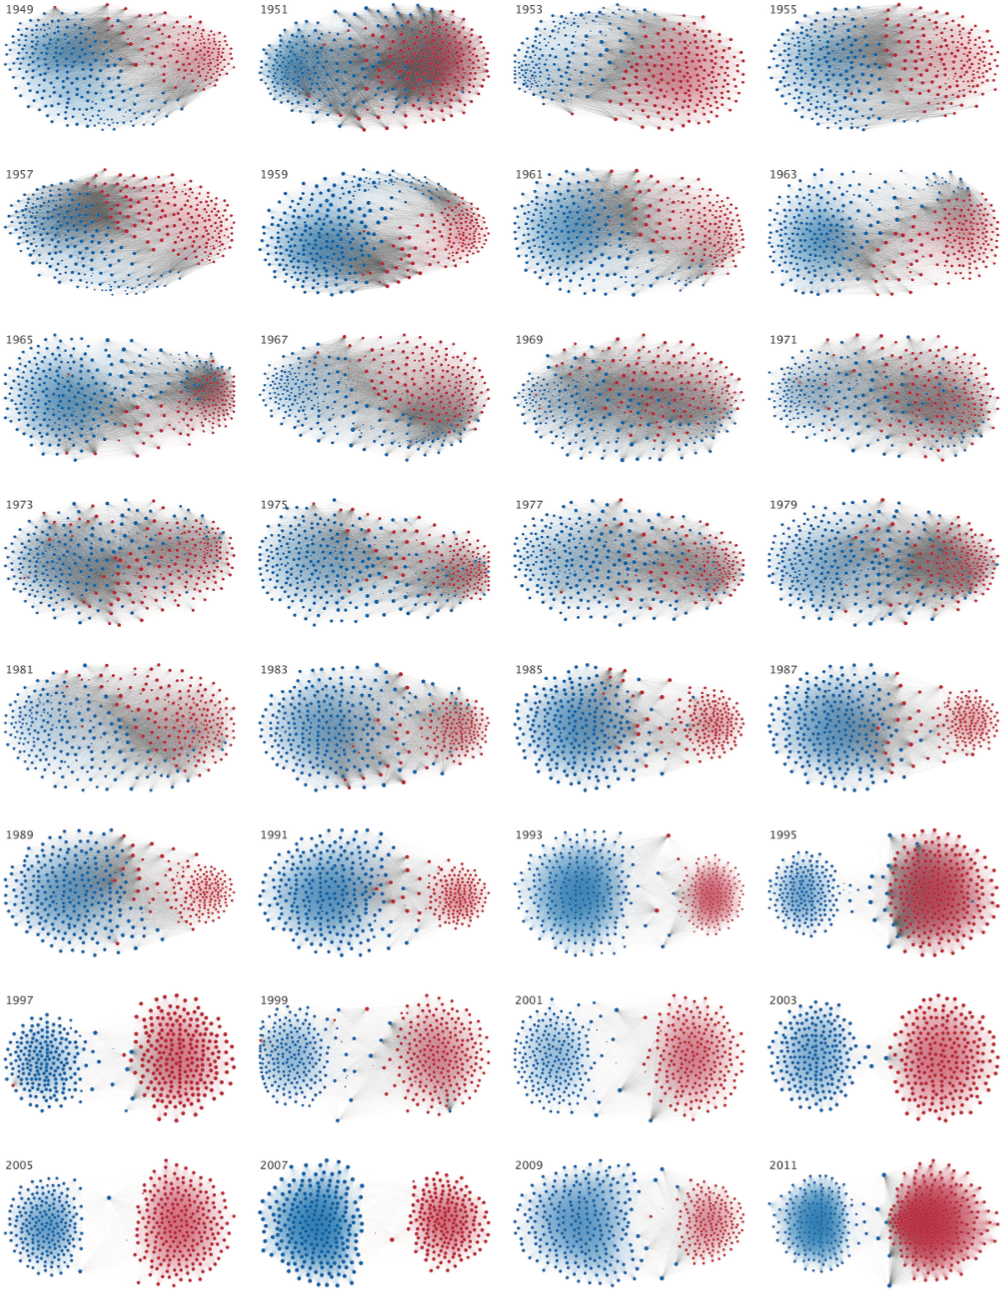
\includegraphics[width=.6\linewidth]{../plots/references/us_parlament.png}
 \caption{Polarization and collaboration in the House of Representatives in the United States. Adapted from \protect\citeA{andris_rise_2015}. Each node represents a member of the U.S. House of Representatives from 1949 to 2012. Each panel shows different two-year congresses with the starting year displayed on top. Republican (R) representatives are in red and Democrat (D) representatives are in blue. When two members agree on more votes than the Congress' threshold, an edge is drawn between them. The Congress threshold reflects the number of agreements, where any pair exhibiting this number is equally likely to be comprised of two members of the same party (e.g. D-D or R-R), or a cross-party pair (e.g. D-R). The size of the nodes reflects their degree, with higher degree nodes being larger.}
 \label{fig:house_of_reps}
\end{figure}

\noindent Despite the decrease in affective polarization in certain northern European countries, polarization globally is on the rise \cite{boxell_cross-country_2020,mccoy_polarization_2018, somer_deja_2018}. There is reason to believe that the general problem of polarization might be getting worse due to technological advances.
Specifically, a growing literature has reported that information is not distributed uniformly across the users of the internet and social media \cite{taylor_exploring_2018, sasahara_social_2021,baumann_modeling_2020,tsai_echo_2020}. Instead, information is being catered to the individual based on their previous search history and behavior on social media \cite{geschke2019triple}. Very different people will therefore be shown very different pieces of information, as users are only presented with a small subset of the available information. 
Heavily influenced by confirmation bias, this can lead to circumstances where almost all opinions one is exposed to are congruent with one's prior beliefs \cite{baumann_modeling_2020}. Such circumstances are popularized under the term echo chambers on social media. Echo chambers are often cited as one of the main reasons for the increase in political polarization \cite{baumann_modeling_2020, sasahara_social_2021, tsai_echo_2020, geschke2019triple}. 

Because of technology's impact on the level of polarization, the internet has been called a mixed blessing \cite{lev-on_happy_2009}. On the one hand, individuals can access more diverse information via the internet, which can help decrease polarization. On the other hand, the internet also enables encounters of extremely opposing opinions by chance, which can increase polarization \cite{lev-on_happy_2009}.

Previous work paints a murky picture concerning the effect of being presented with a set of diverse opinions. The work of \citeA{levy_social_2021} suggests that when people are presented with a diverse set of views, they generally tend to have fewer negative feelings towards other political parties than their own. This result seems to go against the study of \citeA{bail_exposure_2018}, where exposure to directly opposing views can cause opinions to become more polarized than they were before exposure. 
On a similar note, higher involvement in one's echo chamber correlates with more negatively valenced emotions, which suggests that echo chambers are driven largely by outrage. In other words, the most active users in an echo chamber are the ones who are most displeased with the opinions of people outside their echo chamber \cite{del_vicario_echo_2016}.

\noindent Although polarization is usually described in the context of political polarization, polarization is not necessarily a political phenomenon. In fact, polarization can critically impair any social system's ability to cooperate successfully \cite{levin_dynamics_2021}. It is therefore vital to identify and understand what mechanisms can lead a system to polarization, consensus, or anywhere in between the two extremes. This is no easy task. Opinion formation and opinion dynamics are highly complex phenomena \cite{baumann2021modeling}. 
Despite the complexity of the problem, an entire scientific field has been dedicated to the study of how opinions change. The study of the dynamics shaping opinions is aptly named opinion dynamics. The models of opinion dynamics typically assume a static network structure in which agents are situated \cite{galesic_integrating_2021}. By doing so, these models fail to take into account that social networks are dynamic and that the structure of the networks is likely co-evolving with opinions \cite{de2022modelling,galesic_integrating_2021}. The interdependence between the dynamics of social networks and opinion dynamics is largely understudied, despite the fact that the two processes are highly interacting \cite{asikainen_cumulative_2020,bruch_agent-based_2015,galesic_integrating_2021,kossinets_origins_2009,noorazar_classical_2020}. It is therefore not surprising that the dynamic relationship between the two dynamics has often been reported as an important avenue for future research \cite{flache_models_2017,galesic_integrating_2021}. 

\noindent Another important avenue to gain insights into is how to incorporate empirical data in theoretical models \cite{mas2019challenges}. This is an especially pertinent problem in the field of opinion dynamics, which often fails to account for how the results of their models match empirical data \cite{galesic_integrating_2021,flache_models_2017, mas2019challenges}. 
The lack of empirical integration is understandable, as opinions are notoriously hard to measure \cite{mas2019challenges}. Moreover, most of the models of opinion dynamics are not meant to accurately predict how opinions evolve over time, but rather point out interesting interactions between key variables in formal models \cite{mas2019challenges}. Such theoretical models are useful for theory building, but they often run the risk of being too detached from the real world to be useful \cite{smaldino_how_2020, mas2019challenges}.  

\noindent This paper seeks to fill these two critical gaps in the current literature on opinion dynamics: the need to integrate both empirical data and the co-evolution of networks and opinion dynamics. This paper is organized into four parts. The introduction provides an overview of previous methods and vital mechanisms of network and opinion dynamics. This is done by first explaining how agent-based models are well-equipped to investigate complex systems. Next, the critical underlying mechanisms of opinion and network dynamics are identified and introduced. A co-evolutionary agent-based model of opinion and network dynamics is built on the basis of these mechanisms, drawing on insights from data science, social psychology, computational biology, and network science. 
The second part of the paper integrates empirical data into the agent-based modeling process by investigating how well the agent-based model can generate the patterns found in real-world networks. To do so, hyperparameter optimization is employed. This paper expands upon previous use of this technique in agent-based modeling by also implementing a functional analysis of variance (fANOVA) of the hyperparameter importance \cite{hutter2014efficient}. 
The third part of this paper is focused on how co-evolution impacts opinion dynamics. It does so by exploring how the polarization of the system is influenced by the model parameters. This section focuses on understanding how tie-deletion to dissimilar individuals might prevent polarization. 
Finally, the fourth part of the paper discusses the overall findings and presents the key limitations of the model. 

\section{Agent-based modeling of complex phenomena}
The social sciences face the daunting task of trying to explain and predict the behavior of extremely complex systems. 
Historically, social scientists have explained such systems by relying on the power of language using verbal models \cite{smaldino_how_2020}. Verbal models typically explain a system by providing useful analogies, which can help illuminate the system of interest. These analogies are often ambiguous and several interpretations of the same model are possible. The benefit of this ambiguity is that verbal models often incorporate many realistic social and cognitive mechanisms \cite{fogarty_ten_2022}. But ambiguity is often something to be avoided in science, as clarity and precision are necessities for developing useful theories of reality \cite{smaldino_how_2020}. 
Formal models offer an alternative to verbal models, as they offer the kind of precision that is lacking in verbal models at the cost of some realism. Typical examples of formal models are mathematical models, where different variables describe forces in the system \cite{fogarty_ten_2022}. Formal models are especially hard to build for complex systems as the different constituents of the system are hard to reduce to single components \cite{smaldino_how_2020, poli2013note}. Formal models of complex systems often solve this problem by making simplifying assumptions, which reduces the realism of the models \cite{fogarty_ten_2022}. 

Agent-based models are well-equipped to strike a balance between the precision of formal models and the realism of verbal models \cite{flache_between_2018,galesic_integrating_2021,epstein1999agent,mas2014cultural}. This is done by investigating the macro-behaviors of a system, where the micro-behaviors are specified \cite{bruch_agent-based_2015,epstein1999agent,flache_between_2018}. In particular, agent-based models are well-suited when analyzing systems where more is known about interactions between individuals instead of interactions between variables \cite{geschke2019triple}. As is the case with any model, the results critically hinge on the assumptions of the model. It is the role of the modeler to provide as empirically plausible mechanisms as possible for the system of study \cite{crooks2012introduction,epstein1999agent,page2010diversity}. At the same time, the value of a model comes from the fact that it is a simplification of reality. The model should be as simple as it can be and as complicated as it needs to be in order to answer its questions \cite{smaldino_how_2020}. The hope is that by simplifying the system to a sufficient extent, we can observe and understand some important features of even extremely complex systems \cite{fogarty_ten_2022,smaldino_models_2016, smaldino_how_2020, smaldino_models_2022}.

\noindent One of the complex systems that the social sciences have studied for decades is the dynamics governing how opinions are formed and changed \cite{flache_models_2017}. Describing the mechanisms which shape opinion dynamics constitutes a complex problem \cite{mas2019challenges}, in the sense that opinion dynamics is governed by multiple interacting systems. 
How opinions are changed is both the result of how people update their beliefs cognitively and how they are exposed to different perspectives socially \cite{friedkin_social_1990,spears_social_2021}. 

\section{Central Mechanisms}
Investigating the complex system of opinion dynamics is the main aim of this paper. In the following sections, the central mechanisms of opinion dynamics are introduced. The specific focus will be on the tendency for similar individuals to cluster together and on how social relations influence the individual's opinion. 

\subsection{Homophily}
One of the most robust findings of the social world is summed up in the famous phrase "birds of a feather flock together" \cite{mcpherson_birds_2001}. This phrase refers to the fact that assortment in humans is non-random, and is often based on how similar individuals are \cite{asikainen_cumulative_2020,crandall_feedback_2008,mcpherson_birds_2001}. The fact that similarity and social connections are often intertwined is called observed homophily \cite{mcpherson_birds_2001,kossinets_origins_2009}. In all types of human social networks, observed homophily seems ubiquitous.
For all demographic variables which have been investigated, including gender, race, religion, and socioeconomic class, there is always a tendency for more similar individuals to cluster together \cite{asikainen_cumulative_2020,mcpherson_birds_2001, taylor_exploring_2018}. 

\noindent Observed homophily has mainly been explained with a psychological and a structural explanation. The psychological explanation seeks to explain observed homophily by the fact that people seem to exhibit a psychological preference to be with people like themselves. This psychological preference is referred to as choice homophily \cite{asikainen_cumulative_2020,mcpherson_birds_2001,winter_you_2020}.
Such a preference might have evolved as interacting with similar people ensures easier communication and enhances the individual's ability to predict the other person's behavior \cite{kossinets_origins_2009,winter_you_2020}. In this sense, assortment based on similarity could have evolved to facilitate cooperation, because coordination between similar individuals is simpler and less costly for the individual \cite{winter_you_2020,carter2015phenotypic, smaldino2019social}. 

Observed homophily could also be explained by structural constraints. Such constraints could limit how dissimilar choices of interactions are available to the individual \cite{peixoto_disentangling_2022}. As an example, if you work as a female nurse, chances are that most of your interactions at work will be with other females. 
In this case, even if you do not have a strong psychological preference for interacting with people like yourself, the social interactions available to you might primarily be with people similar to you. 
If there is already an existing assortment in a social network, it makes the probability of interacting with similar individuals much higher than with non-similar individuals \cite{peixoto_disentangling_2022}. Such structural factors contributing to observed homophily are referred to as structural homophily \cite{asikainen_cumulative_2020,mcpherson_birds_2001,winter_you_2020}. 

\noindent Observed homophily hints at the prevalent intuition that you have more in common with your friends than you have with strangers \cite{mcpherson_birds_2001}.
Despite its prevalence, few studies have been made to gauge how homophily influences social relations. One such study was made by \citeA{kossinets_origins_2009}, which investigated how observed homophily manifested in real dynamical social networks. They recorded social interactions at a large university for a year. These interactions allowed \citeA{kossinets_origins_2009} to estimate not only how social ties changed over time, but also how similar individuals of the social networks were. Their findings are of significant importance to this paper. First, the results confirm what one might intuitively expect - you have more in common with your friends than you have with strangers. But their findings suggest that this is a special case of a more general phenomenon; that distance in similarity is a function of distance in the social network (see Figure~\ref{fig:distance_similarity}). The further you are removed from someone in the social network, the less you will have in common \cite{kossinets_origins_2009}. 
The connection between distance in similarity and distance in the social network is a robust finding which has also been shown in other large empirical studies \cite{bener_empirical_2016,crandall_feedback_2008}.

\noindent Choice and structural homophily are normally used as separate explanations for the observed homophily in social networks, but they are not mutually exclusive. Rather, it seems that the two processes can facilitate each other \cite{asikainen_cumulative_2020}. For instance, even low amounts of choice homophily could evolve into structural homophily over time \cite{asikainen_cumulative_2020,kossinets_origins_2009,taylor_exploring_2018}. When even a few distant similar individuals connect because of choice homophily, the correlation between proximity and similarity increases. As such, even small preferences will add up over time, and make the correlation between proximity and similarity stronger and stronger, which will lead to increased structural homophily \cite{kossinets_origins_2009}. 
Structural homophily plays a large role as new ties are primarily made to people close to you in the social network \cite{bianconi_triadic_2014, peixoto_disentangling_2022}. When similarity and distance in social networks are connected, structural homophily will increase the observed homophily of the system. Controlling for both distance in the network and shared social circles, generating new social ties is more likely between similar agents \cite{kossinets_origins_2009, bener_empirical_2016}.

\noindent Similarity is not only predictive of which new social ties will be created but also which old ties will be deleted. Although homophily has primarily been studied as a process that makes similar individuals more likely to generate new ties to each other \cite{noel2011unfriending, bener_empirical_2016}, homophily has been shown empirically to also play a key role in tie-deletion. More similar individuals have more stable connections, with a lower propensity to delete ties over time \cite{noel2011unfriending, bener_empirical_2016, mcpherson_birds_2001, kossinets_origins_2009}.
In addition to choice and structural homophily, the connection between similarity and distance is also driven by the increased propensity to delete ties to dissimilar people \cite{kossinets_origins_2009, bener_empirical_2016}. The effect becomes more extreme as interactions between peers tend to make like-minded individuals even more like-minded \cite{friedkin_social_1990, spears_social_2021}. Complementing the empirical studies on tie-deletion, the famous computational work of \citeA{schelling1971dynamic} shows that including even subtle tendencies of tie-deletion of dissimilar pairs can create global patterns of network segregation and community structures that are characteristic of many real-world social networks. 

\begin{figure}[H]
   \centering
   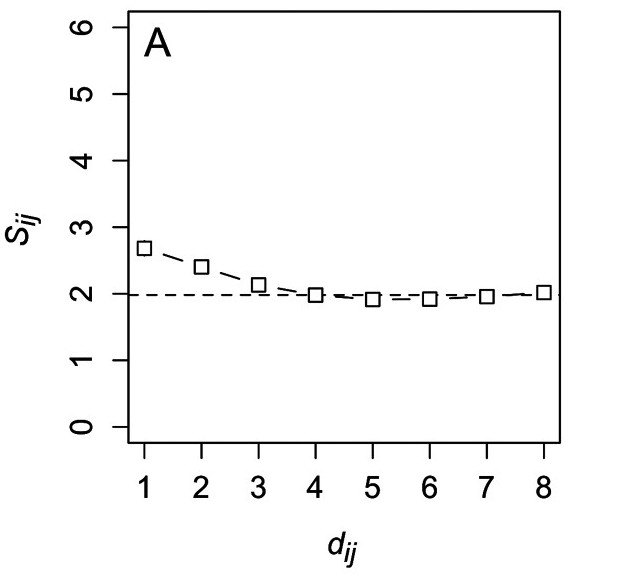
\includegraphics[width=.5\linewidth]{../plots/references/kossinets_watts_distance.jpeg}
 \caption{The link between distance and similarity. Adapted from \ \protect\citeA{kossinets_origins_2009}. The x-axis shows the distance in the network to other agents, $d_{ij}$. The y-axis shows the average similarity between agents, $S_{ij}$.}
 \label{fig:distance_similarity}
\end{figure}

\subsection{Social Influence}
Humans are inherently a social species \cite{kurzban2015evolution}. We do not think and form our opinions in a vacuum. Either via social media, debates, or discussions with friends, opinions are constantly being shared, debated, and discussed with other individuals. 
As a result of these social interactions, the opinions of the people involved in the interaction might change. 
The influence that social encounters and social relations have on the opinions of the involved agents is referred to as social influence \cite{friedkin_social_1990}. Social influence has been proposed as the most important effect in shaping an individual's opinions \cite{chacoma_opinion_2015, flache_between_2018}. As was the case in the previous section, the similarity of individuals is central to how social relations influence opinions. When similar individuals interact, their opinions typically become more similar than they were before interactions \cite{takacs_discrepancy_2016}. On the other hand, dissimilar individuals can repulse each other, which can cause opinions to become more dissimilar from each other than they were initially \cite{hilmert2006positive, cikara2014neuroscience}.  

In this paper, we will distinguish between positive and negative social influence. Positive social influence refers to the force which drives similar individuals to become more similar through interactions \cite{flache_models_2017,levin_dynamics_2021}. 
This can be thought of as instances of reaching a compromise, finding common ground, or seeing the other person's perspective on a topic. Interactions that are driven by positive social influence will be referred to as positive interactions in this paper. Negative social influence refers to the force which causes dissimilar agents to become more dissimilar as a result of interactions \cite{flache_models_2017}. 
Examples include moral outrage or out-group aversion. Interactions that are driven by negative social influence will be referred to as negative interactions in this paper. It is important to note that although positive influence seems to be a robust empirical finding, negative influence is more elusive \cite{flache_models_2017,takacs_is_2014,turner_paths_2018}. 
With that said, there is evidence that suggests that exposure to opposing views can lead to increased polarization \cite{bail_exposure_2018, hilmert2006positive, cikara2014neuroscience}.

\section{Opinion Dynamics}
The field of opinion dynamics attempts to identify key mechanisms which shape how opinions change over time using formal and agent-based models \cite{flache_models_2017,flache_between_2018,noorazar_classical_2020}. Two of the most robustly identified mechanisms are social influence and homophily \cite{flache_models_2017}. The models from opinion dynamics are often analogous, drawing inspiration from statistical physics in the structure and mechanisms of their scientific models \cite{galesic_integrating_2021}. Both continuous and discrete opinions have previously been studied, as well as systems where agents have multiple opinions of interest \cite{flache_models_2017}. The standard approach in opinion dynamics is to use empirical studies of psychological and sociological mechanisms to inform the assumptions of their theoretical models. These models are typically used to identify how these empirically justified parameters interact with each other  \cite{baumann2021modeling,chacoma_opinion_2015,flache_models_2017,friedkin_social_1990,noorazar_classical_2020,spears_social_2021,turner_paths_2018}. By modeling opinion dynamical systems in computational models, researchers create simple systems which represent the more complex and messy real social world. These simplified systems are normally studied to identify which conditions can give rise to polarization or consensus in terms of the opinions of simulated agents \cite{flache_models_2017}.

\subsection{Dynamical networks}
As has already been alluded to in the \textit{\nameref{introduction}}, previous models have focused on social influence without considering how the social interactions change as a result of changes in opinions \cite{galesic_integrating_2021,holme_nonequilibrium_2006,jalili_coevolution_2015}. Central to most classical models of opinion dynamics is that agents are situated in static, theoretical networks \cite{flache_models_2017}. The assumption of static networks is consequential. Real social networks are inherently dynamic, with new ties being formed and deleted over time. As has already been established, empirical work suggests that the processes of opinion and network dynamics are largely interdependent. New social interactions are more likely between similar agents, and tie deletion is more likely between dissimilar agents \cite{kossinets_origins_2009, bener_empirical_2016}. Additionally, it is worth noting that when computational models of static networks include negative social influence, the system cannot overcome polarization of opinions \cite{flache_models_2017, kozma2008consensus}. Previous work has already highlighted how important the assumption of static networks is. Using the mechanism of deleting ties to dissimilar agents, \citeA{kozma2008consensus} shows that co-evolution can create clusters of like-minded individuals which has a large impact on the convergence time of reaching consensus \cite{kozma2008consensus}. 
Although all models do some violence to the world by making assumptions, models should try to include the vital mechanisms of the system they are representing, while simplifying the system enough to understand it \cite{epstein1999agent,smaldino_models_2016}. It is one of this papers's most central claims that the co-evolution of network and opinion dynamics should be considered a vital mechanism. To better explain how opinions are shaped over time, we need to include not only the basic underlying mechanisms of social influence but also network dynamics. 

\section{Network Dynamics}
Models of opinion dynamics typically situate the agents of their models in static, theoretical networks \cite{flache_models_2017, galesic_integrating_2021}. Classic examples of the networks used in most models of opinion dynamics include ring lattices, small-world networks and scale-free networks \cite{barabasi_scale-free_2003,watts_collective_1998}. Both small-world and scale-free networks are famous for being able to capture essential features of real social networks. Small-world networks are able to capture the general tendency of high average clustering coefficient and low average path length found in most social networks \cite{watts_collective_1998}. This is achieved by starting with a ring lattice and rewiring a small percentage of the ties randomly. Randomly rewiring a few ties creates highways of information which decreases the average path length considerably \cite{watts_collective_1998}. Scale-free networks can capture the general tendency of long tails in the degree distributions of social networks. The degree distribution of social networks often follows a power law, where a few nodes have an extremely high amount of edges, while most nodes only have a few \cite{barabasi_scale-free_2003}. Recent work calls into question how universal power laws are in empirical social networks and finds instead that most degree distributions from social networks follow a log-normal distribution \cite{broido_scale-free_2019}. Note that neither of the most used theoretical networks can generate all the essential features of social networks \cite{jacksonsearch2004}. Small-world networks have unrealistic degree distributions, and scale-free networks have very low average clustering coefficients. 

\subsection{Triadic Closure}
Both scale-free and small-world networks attempt to answer the question of how network characteristics could be generated, not why social networks have the characteristics that they do \cite{jacksonsearch2004}. An attempt at answering the why-question is the work by \citeA{jacksonsearch2004}, which emphasizes the role of triadic closure in network generation. Triadic closure refers to making new connections by generating new ties to "friends of friends", i.e. the edges of one's edges (see Figure~\ref{fig:tie_closure}). Reliably, triadic closure is found to be the most important and robust mechanism for how new connections are made in social networks \cite{asikainen_cumulative_2020,bianconi_triadic_2014,kossinets_origins_2009,peixoto_disentangling_2022}. Empirical studies on dynamical networks find that the probability of creating a new tie is a decreasing function of the distance in the network \cite{bener_empirical_2016,kossinets_origins_2009}. The less separated you are from someone, the more likely you are to form a social tie with this person. A popular colloquial framing for distance in social networks is to measure distance between individuals in "handshakes" \cite{smith2005networks}. One's friends are one handshake away, friends of friends are two handshakes away and so on. The empirical studies suggest that when you are two rather than three handshakes away from someone, you are 30 times more likely to form a connection (see Figure~\ref{fig:tie_closure}). This increase in likelihood only becomes more extreme when the distance is increased. When you are two rather than five handshakes away from someone, you are 2.500 times more likely to form a connection \cite{kossinets_origins_2009}. 

\subsubsection{Triadic closure and network metrics}
Using triadic closure as the generating principle for network formation has shown great promise in explaining some key characteristics of social networks \cite{ilany_social_2016}. In previous formal models of network formation, this is implemented by making most new connections via triadic closure while letting a few connections be made at random \cite{ilany_social_2016,jacksonsearch2004,jacksonmeeting2007}. These models can generate the important characteristic findings in social networks of high average clustering coefficient, low average path length and log-normal degree distributions \cite{jacksonsearch2004,jacksonmeeting2007}. 

\noindent It is worthwhile to pause to understand why these network metrics are important and why triadic closure might generate patterns akin to those of empirical social networks. The average clustering coefficient is a measure of how connected local communities are in networks \cite{watts_collective_1998}. Social networks typically exhibit high average clustering coefficients, which is closely linked to the fact that social networks typically consist of a number of tight-knitted, well-connected local communities \cite{peixoto_disentangling_2022, newman_finding_2006, crandall_feedback_2008}. Models of triadic closure are likely to exhibit high average clustering coefficients, as triadic closure will increase the number of local links \cite{jacksonmeeting2007}. 

The average path length refers to the average length of the shortest path between any two nodes in a network \cite{watts_collective_1998}. The average path length is important for how fast information or contagious diseases can spread in a network \cite{cowan2004network}. Social networks typically have low average path lengths, where no individual is many handshakes away from being connected to another individual \cite{backstrom2012four}. The network formation models using triadic closure also have low average path lengths, benefiting from similar mechanisms of randomness as small-world networks to achieve low average path lengths \cite{jacksonmeeting2007,watts_collective_1998}. As mentioned, a small amount of randomness can create long-range connections, which decreases the average path length substantially \cite{watts_networks_1999}.  

Finally, the degree distribution is the distribution of the number of edges each agent has in a network. As mentioned, social networks typically have log-normal or scale-free degree distributions. In networks with such degree distributions, some nodes will have a very large degree, while most nodes will have a relatively low degree \cite{bianconi_triadic_2014}. These types of degree distributions are generated via triadic closure. The reason is that triadic closure is a mechanism where the probability of generating a new connection is proportional to how many connections a node already has. High degree nodes have more possibilities for being selected for via triadic closure simply because they have higher degrees \cite{jacksonmeeting2007}. Similarly, low degree nodes will have fewer connections that could generate new ties with them via triadic closure. This effect is similar to the mechanisms of preferential attachment in scale-free networks \cite{barabasi_scale-free_2003}.

\begin{figure}[H]
   \centering
   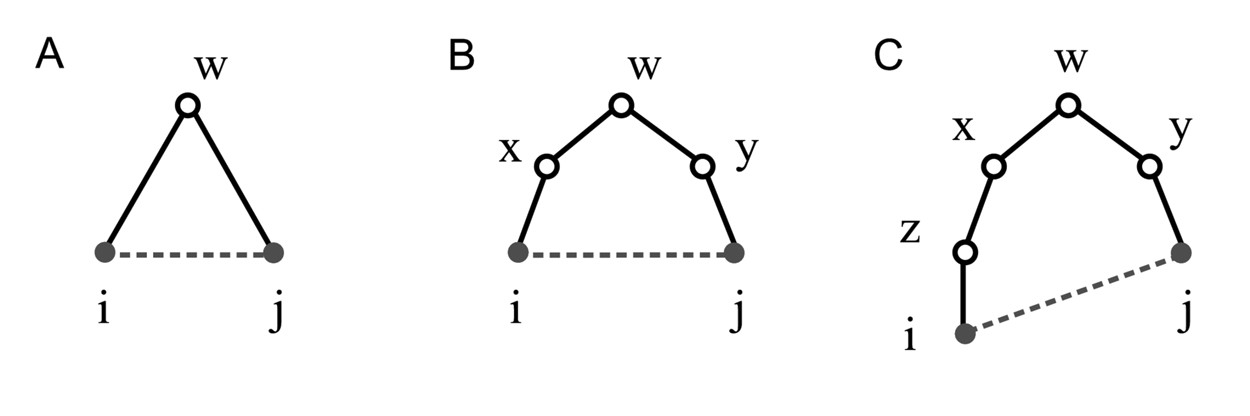
\includegraphics[width=.8\linewidth]{../plots/references/kossinets_watts.jpeg}
 \caption{Different types of tie closure. Taken from \protect\citeA{kossinets_origins_2009}. Panels show different ways of creating social ties via existing connections. Creating social ties in this way is often called tie-closure. Panel A depicts closing ties with a friend of a friend. This type of tie closure is called triadic closure. Panel B and C show longer cycles of closure.}
 \label{fig:tie_closure}
\end{figure}

\section{Co-evolution via tie-deletion}
Up until now, opinion and network dynamics have been presented and discussed in isolation. But as mentioned, these dynamics are known to be interdependent \cite{bener_empirical_2016, kossinets_origins_2009, galesic_integrating_2021}.
It is easy to see how opinions could be influenced by network dynamics. 
As the social network changes, the available interactions for each agent will change. 
As one of the primary forces of opinion dynamics is social influence \cite{levin_dynamics_2021, chacoma_opinion_2015}, changes in the social network will have large effects on the opinions of the social agents of the network. 
As the social network already influences opinion dynamics, any mechanism that changes the ties in the network based on the opinions of the agents will cause opinion and network dynamics to co-evolve. 
There are good reasons to believe that such mechanisms are numerous \cite{bener_empirical_2016, kossinets_origins_2009, levin_dynamics_2021}.
In this paper, the co-evolutionary mechanism considered will be the tie-deletion of dissimilar individuals. 
Tie deletion of dissimilar individuals has been shown empirically to be a robust phenomenon \cite{kossinets_origins_2009, bener_empirical_2016}. Moreover, this mechanism has been studied previously in similar models to the one presented in this paper \cite{santos_cooperation_2006,sasahara_social_2021}. 
By using a tie-deletion as the co-evolutionary mechanism, we can better assess the robustness of the current claims in the literature. 

\subsection{The effect of tie-deletions on cooperation}
The previous studies on how tie-deletion influences cooperation do not come exclusively from the field of opinion dynamics. For instance, the field of computational biology is especially keen on identifying what conditions must be satisfied to facilitate the evolution of cooperation. Computational biology should be considered an adjacent field to opinion dynamics, as they share much in their interests and in their methods \cite{dakin_dynamic_2018,melamed_strong_2016,pepper_mechanism_2002,santos_cooperation_2006, smaldino2019social}. 

\subsubsection{Tie-deletion facilitates cooperation}
\noindent In one of the studies from the field of computational biology, \citeA{santos_cooperation_2006} studied how social connections are linked to whether a system of agents can cooperate. Intuitively, one might expect that when a network of social actors becomes more connected, levels of cooperation in the system should increase. However, the opposite effect is observed. In their paper, \citeA{santos_cooperation_2006} consider agents playing game-theoretic games, where agents either cooperate or defect. 
\citeA{santos_cooperation_2006} analyze what happens when agents adjust their ties based on the interactions made with other agents. When cooperators interact with defectors, the social tie between cooperators and defectors has a chance of being rewired to a different agent. This keeps the number of edges constant but decreases how globally connected the network is \cite{santos_cooperation_2006}. Their results indicate that cooperation flourishes when the propensity for deleting ties between cooperators and defectors increases (see Figure~\ref{fig:santos}). The interpretation given by \citeA{santos_cooperation_2006} is that removing ties between cooperators and defectors increases positive assortment between cooperators and decreases positive assortment between defectors and cooperators. One of the striking attributes of this finding is that without any propensity for tie-deletion, cooperation does not evolve for conditions equivalent to the Prisoner's Dilemma \cite{santos_cooperation_2006}. More generally, positive assortment has been found to be a robust facilitator of cooperation in computational biology \cite{boyd_coordinated_2010,dakin_dynamic_2018,melamed_strong_2016,pepper_mechanism_2002}. As an aside, \citeA{santos_cooperation_2006} also show that using even relatively simple principles of co-evolution, where network dynamics reflect the individual agent's reaction to their social interactions, can produce realistic social networks \cite{santos_cooperation_2006}. 

\begin{figure}[H]
   \centering
   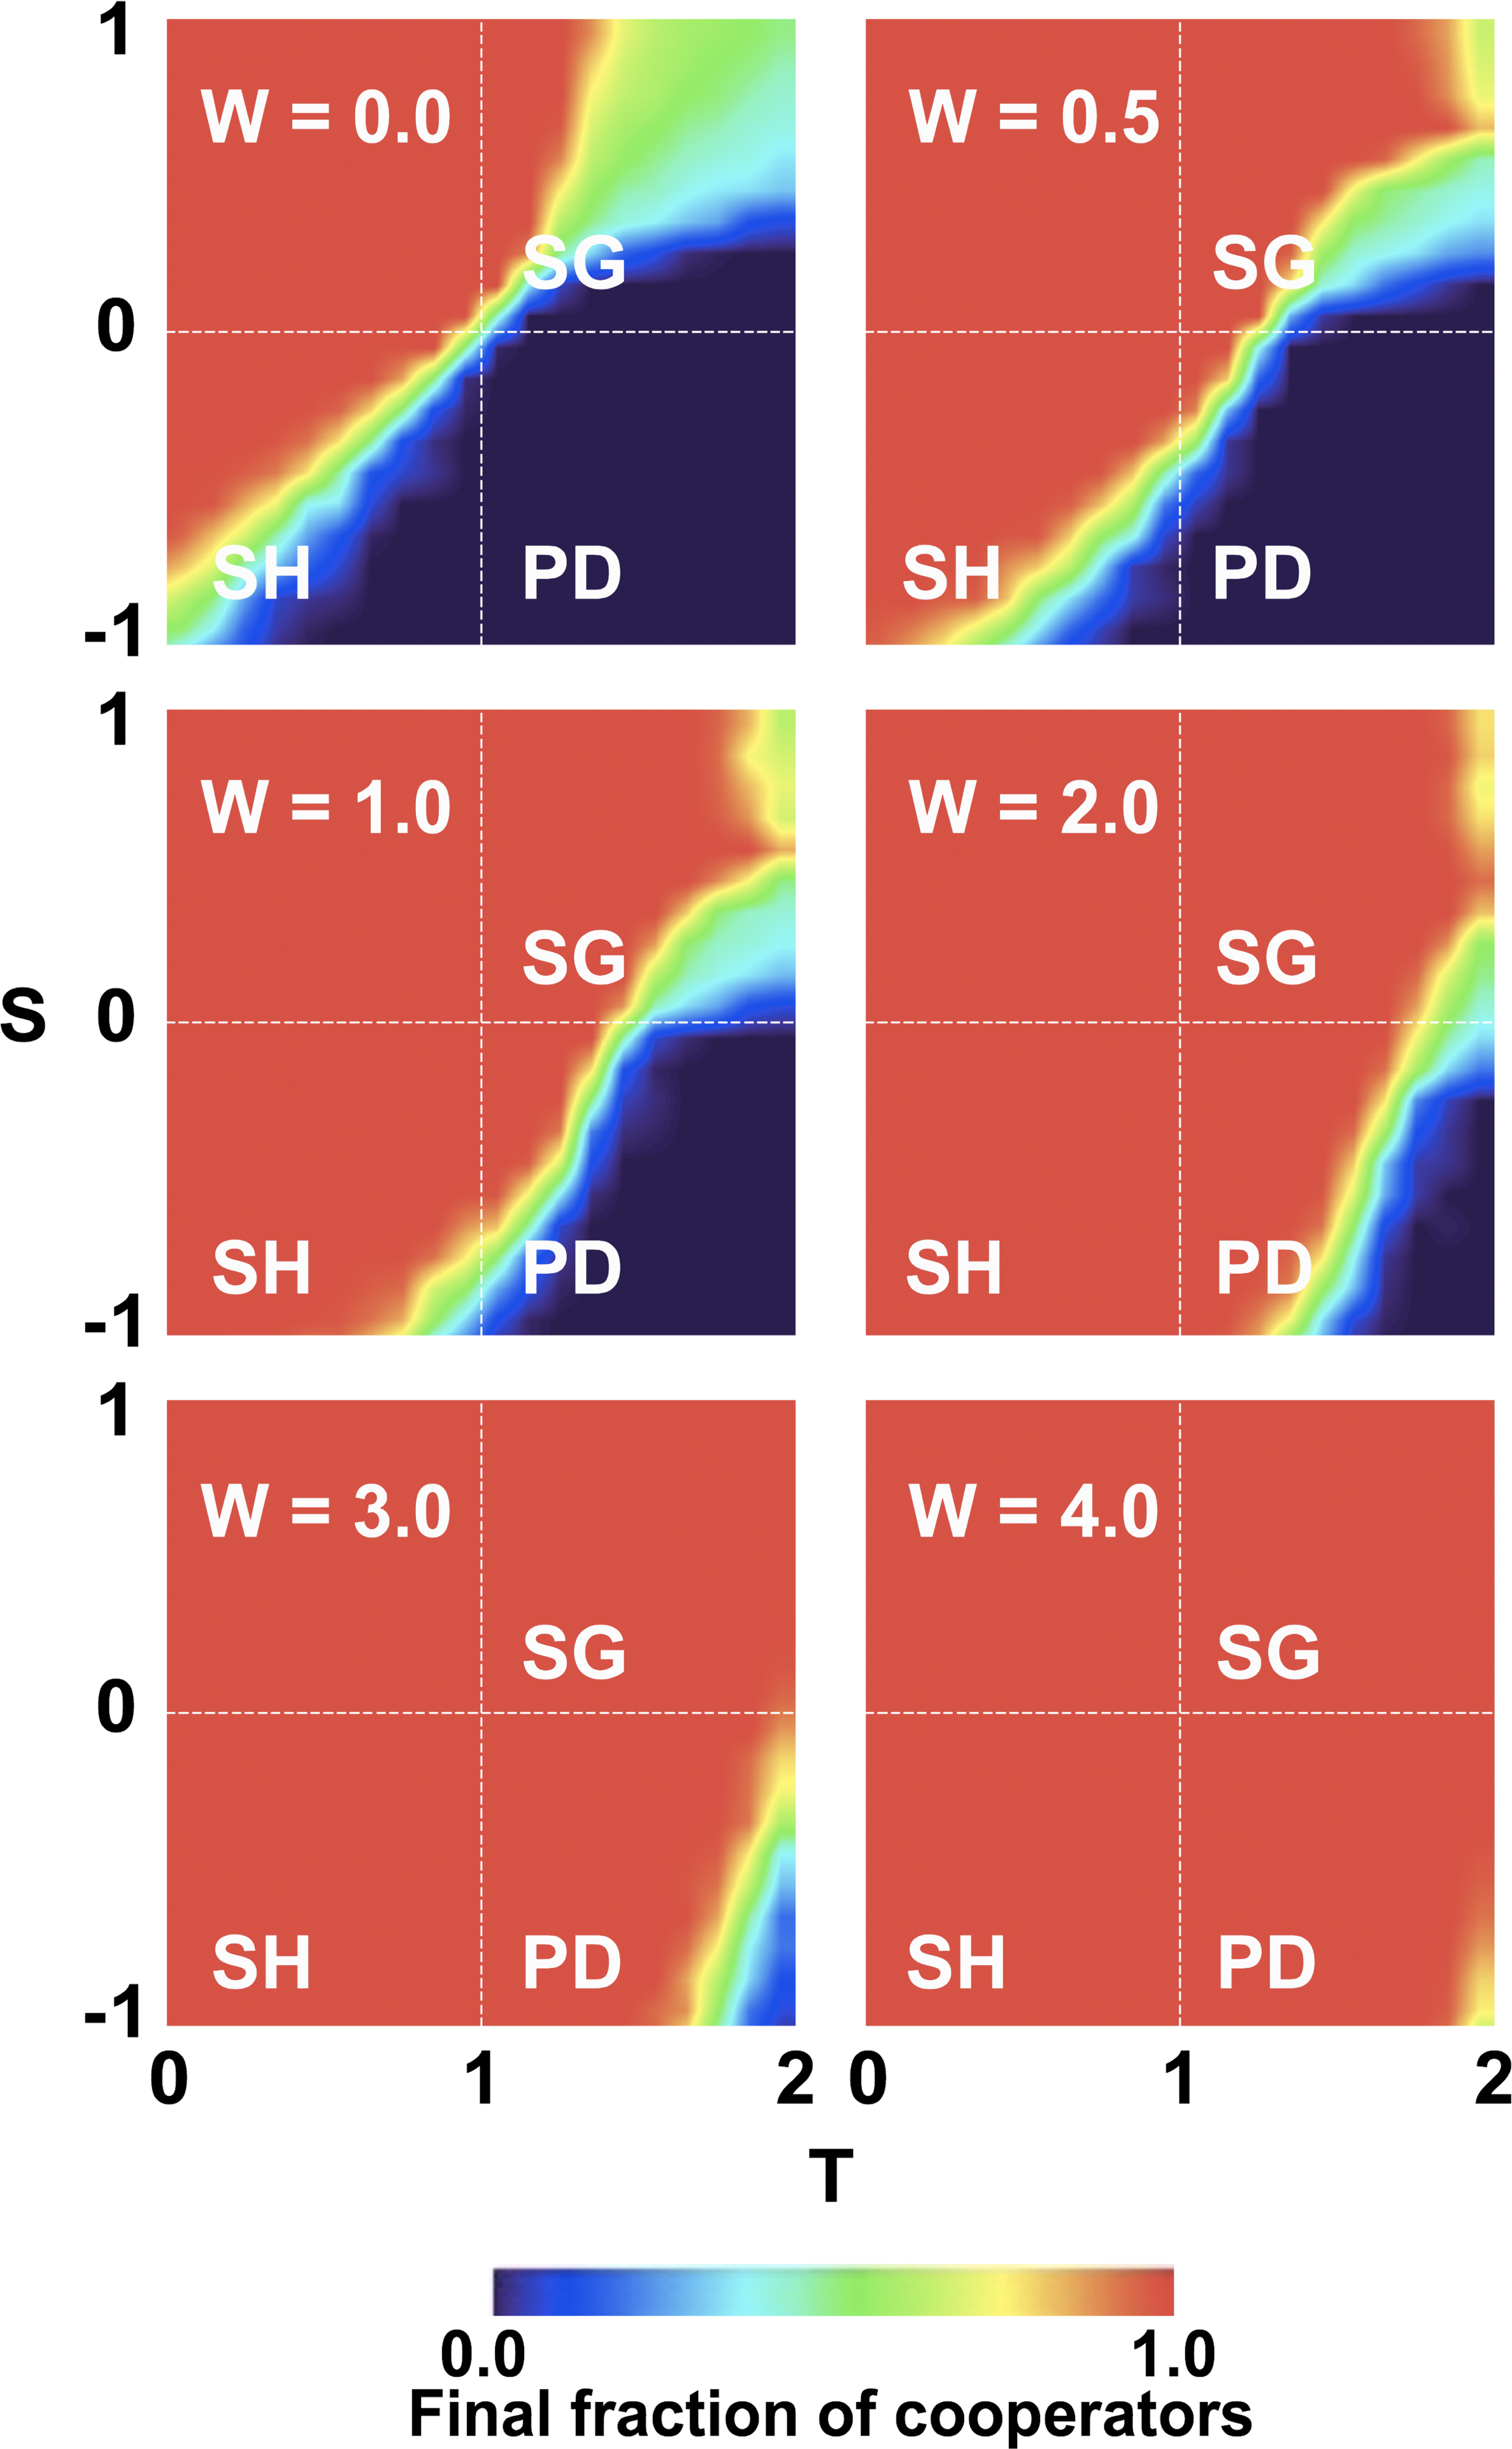
\includegraphics[width=.4\linewidth]{../plots/references/santos.png}
 \caption{Tie-deletions facilitate cooperation. Taken from \protect\citeA{santos_cooperation_2006}. Panels show simulations with different values of $W$. In the model of \protect\citeA{santos_cooperation_2006}, $W$ controls the propensity to delete ties between defectors and cooperators. Increases in $W$ lead to more rewiring of connections between defectors and cooperators. The y-axis shows the disadvantage of being cheated, and the x-axis shows the pay-off of cheating. The letters on the panel represent well-known game-theoretic dilemmas (Prisoners Dilemma, Stag Hunt, and Snow Drift Game). Colors show the final fraction of cooperators after simulations are completed. When $W = 4.0$, cooperators wipe out defectors. }
 \label{fig:santos}
\end{figure}

\subsubsection{Tie-deletion accelerates echo chambers}

\noindent Although the effect of positive assortment on cooperation seems general in the computational biology literature \cite{boyd_coordinated_2010,dakin_dynamic_2018,melamed_strong_2016,pepper_mechanism_2002}, some models from opinion dynamics point to an opposite result. When combined with social influence, \citeA{sasahara_social_2021} report that tie-deletion between dissimilar agents accelerates polarization by generating echo chambers that stifle cooperation (see Figure~\ref{fig:echo_chambers}). This is in line with the more intuitive explanation, where a decrease in communication between agents leads to a decrease in cooperation. Similarly, this is also in line with the research on echo chambers, where isolation leads to further polarization \cite{tsai_echo_2020, del_vicario_echo_2016}. 

\noindent It is noticeable that the same underlying mechanism can cause so drastically different results in the two models. For both studies, tie-deletion is a critical mechanism, but they find opposing directions of the effect \cite{santos_cooperation_2006,sasahara_social_2021}. It is precisely because of this dispute that further research should be made on how the deletion of negative ties can impact cooperation.

\begin{figure}[H]
   \centering
   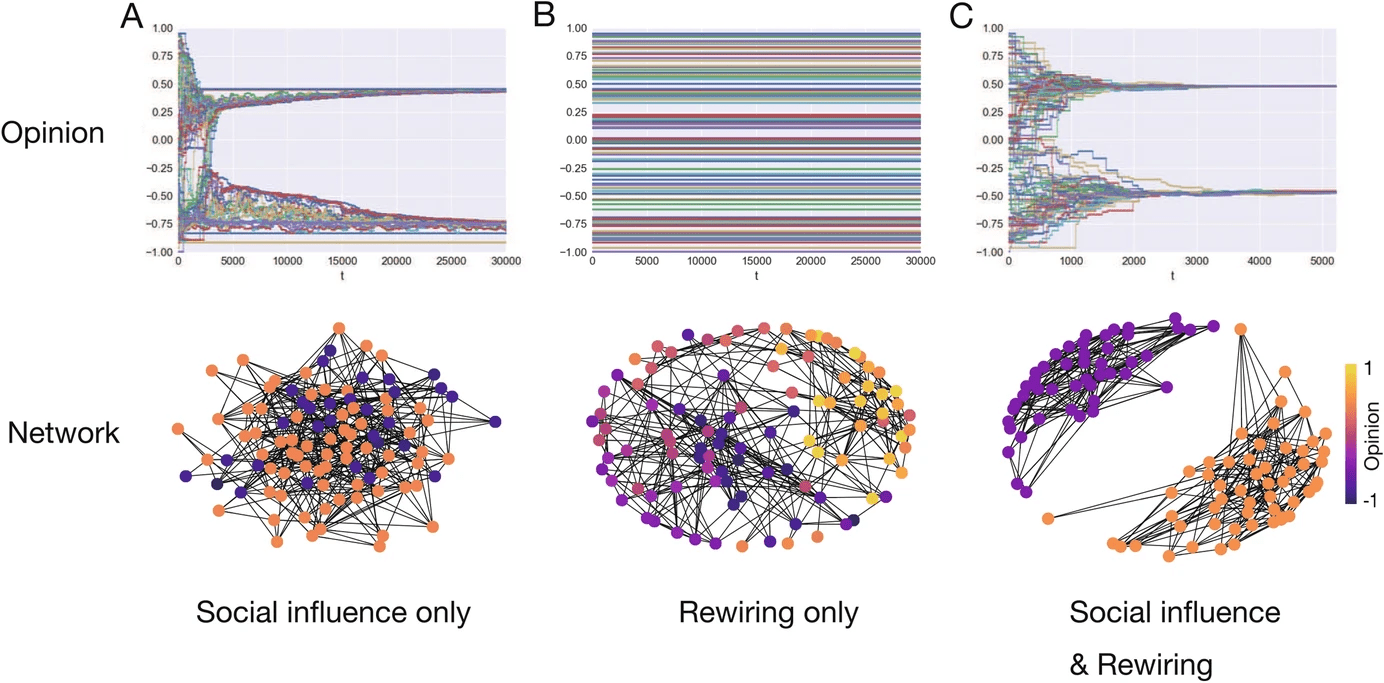
\includegraphics[width=.8\linewidth]{../plots/references/echo_chambers.png}
 \caption{Tie-deletion accelerates polarization. Taken from \protect\citeA{sasahara_social_2021}. The first row shows the trajectory of opinions over time and the second row shows the network after simulation. Columns show simulations of different conditions. Column A shows the results from only including social influence. Column B shows the results from conditions that only rewire connections based on opinions. Column C shows the results of including both social influence and rewiring. Of special interest is the last column, which shows that tie-deletion can accelerate echo chamber formation, as the opinions stabilize faster than when only social influence is included.}
 \label{fig:echo_chambers}
\end{figure}

\section{Model Description}
The following section describes the agent-based model of opinion and network dynamics based on the key mechanisms of homophily, social influence, triadic closure, and tie-deletion. First, a conceptual overview of the model is provided, followed by a description of the key assumptions of the model. Thereafter, the specific steps which govern the behavior of the agents of the model at each time-step are explained in detail. 

\subsection{Conceptual overview}
The agent-based model presented here represents a system where social agents interact with their peers and discuss their opinions with each other. The system of interest is a social system where agents change not only their opinions but also their social ties. To represent these social ties, the agents are situated in an undirected and unweighted network, where nodes of the network represent social agents and edges represent social ties between agents. The fact that the network is undirected means that all relations between agents are reciprocal. This way of representing connections between social agents results in a system where you cannot be friends with someone if they are not friends with you. Similarly, the fact that the network is unweighted means that no connections are stronger or weaker than others. 


\subsection{Assumptions}
The model makes several assumptions to simplify the processes of opinion and network dynamics. It is assumed that the opinion of an agent is shaped only by her initial opinion and the influence of her peers. 
The model does not assume that the agents of the system have any tasks to perform or strategies to follow. Agents are not trying to find any "true opinion" or act in a way to hide their own opinion from their peers. Instead, the agents are assumed to share their opinions truthfully to other agents, and to be able to perceive the exact opinion of their connections. 
In line with previous models of opinion dynamics, the model assumes positive social influence between agents of similar opinions. In other words, agents of similar opinions will reach a compromise which pulls their opinions closer together. Similarly, the model assumes either negative or no social influence between dissimilar agents. Agents will either not be influenced at all, or they will further distance themselves from agents with dissimilar opinions from their own. Regarding the social network of the model, it is assumed that agents will find new connections primarily through their already existing connections via the mechanism of triadic closure. Finally, it is assumed that agents will tend to delete ties to dissimilar agents.
All these assumptions can vary in the strength of the proposed effect. Take for instance the effect of positive social influence. A strong force of positive social influence would result in agents reaching a perfect compromise, while a weaker force would result in agents that barely influence each other. 
As the results of the model depend on the strength of these assumptions, they are controlled for explicitly by the parameters of the model. 

\subsection{The stages of the model}
The agent-based model is divided into three distinct and sequential stages, which are executed at every time-step.
In essence, every time-step consists of an agent first creating new social ties, sharing their opinions with their existing connections and then deleting dissimilar ties.
These stages are referred to as the network dynamic stage, the opinion dynamic stage, and the co-evolutionary stage respectively: 

\begin{itemize}
    \item The network dynamic stage specifies how new edges are created in the social network of the model. The behavior of this stage of the model is controlled by one parameter, $R$. $R$ specifies the probability of generating random ties rather than ties via triadic closure.
    \item The opinion dynamic stage describes how interactions between agents change their opinions via social influence. The opinion dynamics are controlled by three parameters, $T$, $\alpha$, and $\beta$. $T$ specifies the threshold for what constitutes a similar agent, $\alpha$ specifies the power of positive social influence and $\beta$ specifies the power of negative social influence.
    \item Finally, the co-evolutionary stage specifies the tendency for agents to delete connections to dissimilar agents. This is controlled by the parameter $P(D)$, which describes the probability of deleting ties to dissimilar agents.
\end{itemize}

\noindent The specifics of each stage of the process are introduced in detail in the section called \textit{\nameref{dynamics}}. While we mainly focus on one agent-based model, we develop two models. 
One of the models considered is an agent-based model which only contains the network dynamic stage as described above. This model serves as the baseline for the full co-evolutionary model, which includes all three stages described above. The comparison between these two models will be a central part of the discussion on the integration of empirical data. We will refer to the model that only includes the network dynamic stage as the Network Formation Model and the model with all three stages as the Co-evolutionary Model (see Figure~\ref{fig:flowchart}).

\begin{figure}[H]
  \centering
  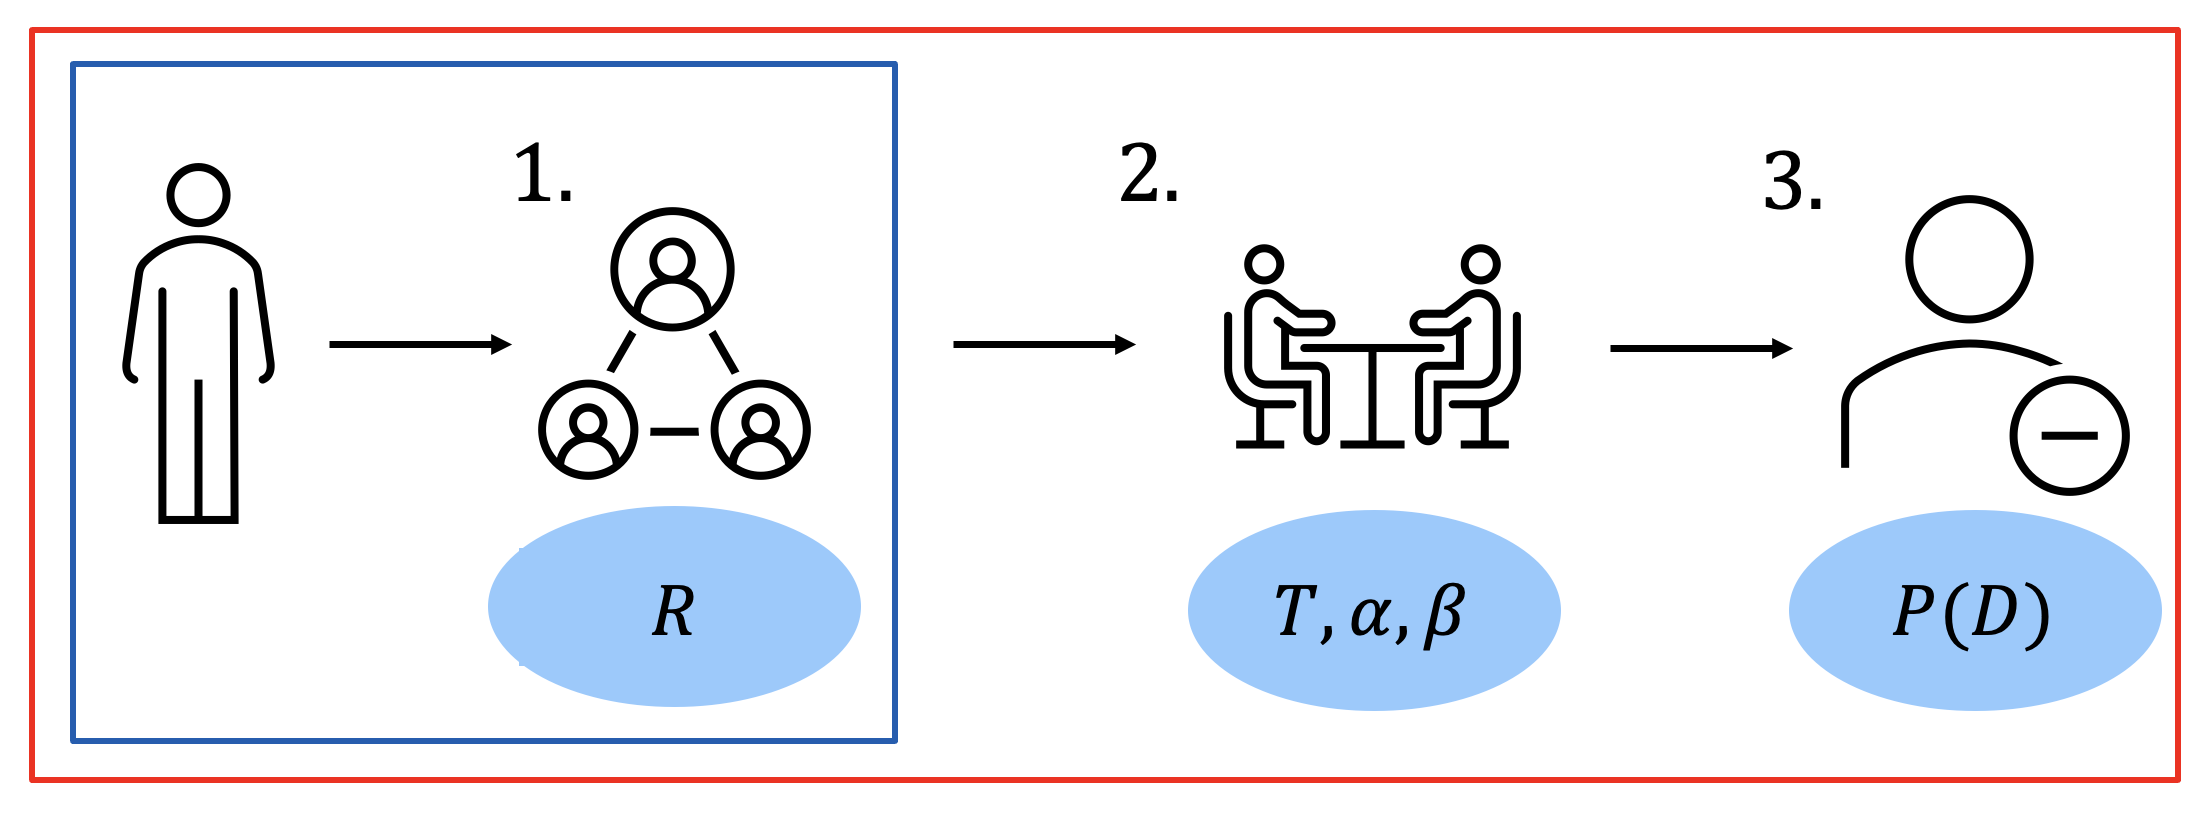
\includegraphics[width=.9\linewidth]{../plots/schematics/model_representation.png}
\caption{Flowchart of a single time-step. The numbers indicate different stages of a single time-step. The squares of different colors show the time-step of different models. The blue square shows a single time-step for the Network Formation Model and the red square shows a single time-step for the Co-evolutionary Model. Cyan bubbles show what model parameters are relevant to the particular model stage. A time-step starts with sampling a random agent, $A_t$, from the network. Next, the network dynamic stage (1) begins where a new connection is made from $A_t$ to another agent. Whether the connection is made randomly or via triadic closure is controlled by $R$. This is the only stage included in the Network Formation Model. After the network dynamic stage, the Co-evolutionary Model begins the opinion dynamic stage (2). The sampled agent, $A_t$, pushes and pulls on the opinions of neighboring agents. This is controlled by a threshold for similarity, $T$, and forces of positive and negative social influence, $\alpha$ and $\beta$. After this process, the co-evolutionary stage begins (3). With a probability of $P(D)$, ties to agents with an opinion further than $T$ apart from $A_t$'s opinion are deleted. This concludes one time-step of the Co-evolutionary Model.}
\label{fig:flowchart}
\end{figure}

\subsection{Initialization}
The model has a set of requirements that must be initialized before it can function as intended. The first of which is that for social agents to be social, they need a social scene to act on. Therefore, agents are initially situated in a random Watts-Strogatz small-world graph \cite{watts_collective_1998}. For all models presented in this paper, all initial small-world graphs are generated with a rewiring probability of $p=0.5$, while the number of nodes, $N$, and number of initial connections, $k$, are varied \cite{watts_collective_1998}. The choice of the initial network is made due to the fact that small-world networks are a typical choice in the literature of opinion dynamics \cite{turner_paths_2018, flache_models_2017}.

The second initial requirement of the model is that the agents must have some opinions to share with their peers. Each agent is given a number on a continuous scale between -1 and 1, which is taken to represent her initial opinion, $O_I$. By having opinions represented continuously, opinions can be anything between extremely pro or extremely against some notion. 
In line with previous research, the initial opinions of agents are assumed to be diverse \cite{galesic_integrating_2021, flache_models_2017, flache_between_2018}. To implement the diversity of initial opinions, all values of $O_I$ are initialized by drawing from a uniform distribution between -1 and 1: 

$$O_I \sim U(-1, 1)$$

\subsection{Dynamics}
\label{dynamics}
To investigate how the processes of network and opinion dynamics influence each other over time, agents iteratively interact with each other over the course of a number of discrete time-steps. 
In the real world, social agents are constantly interacting, with multiple interactions happening at the same time. This causes problems in simulation models, as synchronous updating of opinions has been reported to cause dramatic instability \cite{flache_models_2017, sasahara_social_2021, galesic_integrating_2021}. For this reason, this model follows previous conventions and updates opinions asynchronously. To do so, a random agent is sampled from the network to be the agent on turn, $A_t$, at every time-step. 
Formally, let $t$ specify the time-step of the agent-based model, $A_t$ be the agent on turn at time-step $t$ and let $S_t$ be the network at time-step $t$.

As $A_t$ is a randomly sampled agent at every time-step, $A_t$ can in principle be the same agent for all time-steps. To ensure that the sampling is more evenly distributed across all agents, the maximum number of time-steps, $t_{max}$, is proportional to the number of agents in each simulation, $N$. This is standardized across different network sizes by specifying that all agents are expected to be the agent on turn 10 times during the course of one simulation. Note that even with the inclusion of this property of the model, some agents will have more time-steps as the agent on turn than others. As each model simulation uses different random seeds, this disparity will be negligible. For all simulations considered in this paper, the model terminates when $t = t_{max}$, where $t_{max}$ is defined as 

$$t_{max} = 10 \cdot N$$

\subsubsection{Network dynamic stage}
\label{network dynamic stage}
The first stage of the model represents how social agents find new connections in social networks. These new connections are primarily generated via triadic closure, while a subset of new connections will be generated randomly. The balance between triadic closure and randomness is controlled by the parameter $R$. $A_t$ connects to a random agent that $A_t$ is not currently connected to with a probability of $R$. 
Similarly, $A_t$ connects to one of its edge's edges that it is not currently connected to with a probability of $1-R$. If $A_t$ is already connected to all its edges' edges, and is supposed to make a new connection via triadic closure, $A_t$ does not create a new edge. The lower the value of $R$, the more new ties are generated via triadic closure. 

\noindent Some intricacies concerning the network dynamic stage are worth noting, as later stages of the model can delete social ties. This is consequential as the number of ties in the network is likely to be an important factor and therefore needs to be controlled for. 
To keep the number of edges in the network approximately constant, new edges are either created or rewired to account for deleted edges. 
This is done by ensuring that when the number of edges in the network is lower than the initial number of edges in the network, new edges are created and not rewired. When the number of edges in the network is the same number as the initial number of edges in the network, new edges are rewired instead. As a consequence, the network can have fewer edges than it had initially but never more. 
Formally, this is achieved by letting $E_1$ be the number of edges of $N_1$ and letting $E_t$ be the number of edges of $S_t$. 
If $E_t < E_1$, $A_t$ will not rewire one of its existing edges, but instead create a new edge. If $E_t \geq E_1$, $A_t$ will rewire one of its existing connections when new social ties are made.

\noindent Rewiring of edges or deletion of ties can cause the network to separate completely into distinct components where no links exist between members of different components. Although complete segregation of networks likely occurs in the real world (see Figure~\ref{fig:house_of_reps}), having multiple components complicates network analysis extensively. For instance, the average path length of the social network is an important measure of this study, but it is only rigorously defined for networks of a single component. When a network only has one component, there exists a path between any two nodes of the network. To simplify the network analysis and allow for the calculation of the average path length, the model is restricted to only having one component. 

Formally, this is done by letting $C$ define an agent that lost its connection with $A_t$ via either rewiring or tie-deletion. To check whether $S_t$ has multiple components, the degree of $A_t$ and $C$ is calculated. If the degree of either $A_t$ or $C$ is 0, these agents constitute a second component on their own. In this case, a new edge is created randomly from the agent that has a degree of 0 to a new node from $S_t$.  
If both $A_t$ and $C$ have degrees larger than 0, and $S_t$ has more than one component, a new edge is created to merge the two components together. Specifically, the edge that $A_t$ rewired or deleted from $C$ is restored.
When $A_t$ rewires its edges, $A_t$ will not connect to new agents if an edge was created to ensure that $S_t$ only has one component.
I will refer to the process of ensuring only one connected component simply as component insurance. 

\subsubsection{Opinion dynamic stage}
After creating a new social tie, the agents interact with each other. This is meant to represent discussions or other social interactions between agents. During such interactions, positive and negative social influence will have an effect on the opinion of the agents. 
To model social influence, the agent on turn, $A_t$, interacts with all her connected agents iteratively and changes her opinion and theirs. 
As the ordering of interactions between the edges of $A_t$ could be important for the resulting change in opinions, the order of interactions is randomized. Whether other social agents are similar enough to reach a compromise with $A_t$ is decided by a threshold value, $T$. When the distance between the opinions is lower than $T$, positive social influence will pull these opinions closer together. If the distance is larger than $T$, negative social influence will push the opinions further apart.
Representing this formally, let $B$ denote an edge of $A_t$ and let $O(\cdot)$ define a function with agents as inputs and their opinions as outputs.
When $T \geq \abs{O(A_t) - O(B)}$, the interaction between the two agents will be positive and as a result, the opinions of the two agents will be pulled closer together. The force with which they are pulled is the positive social influence, $V_p$, which is defined as a fraction of the distance between opinions. How much of the fraction opinions are pulled towards each other is controlled by the parameter $\alpha$:

$$V_p = \big(\abs{O(A_t) - O(B)}\big) \cdot \frac{\alpha}{2}$$

Let $O_{max} = \max \big(O(A_t), O(B)\big)$ and $O_{min} = \min \big(O(A_t), O(B)\big)$ and update the values of opinions by:

$$O'_{max} = O_{max} - V_p$$
$$O'_{min} = O_{min} + V_p$$

where $O'_{max}$ and $O'_{min}$ are the updated values of $O_{max}$ and $O_{min}$ respectively after the agents have interacted with each other. When $T < \abs{O(A_t) - O(B)}$, the interaction will be negative. The opinions of the two agents will be pushed further apart by the power of negative social influence, $V_n$, via a principle similar to positive social influence. With negative social influence, how much of the fraction they are pushed apart is controlled by the parameter $\beta$: 

$$V_n = \big(\abs{O(A_t) - O(B)}\big) \cdot \frac{\beta}{2}$$

Using the same definitions as above, the opinion of each agent is updated:

$$O'_{max} = O_{max} + V_n$$
$$O'_{min} = O_{min} - V_n$$

\noindent As the model represents opinions on the spectrum between -1 and 1, the opinions after interacting are also restricted to fall within this spectrum. If an agent's opinion becomes larger than 1 after interacting with other agents, their updated opinion is replaced with the number 1. Similarly, if their opinion becomes lower than -1, their opinion is replaced with the number -1. Before moving on to the co-evolutionary stage of the model, there are some aspects of this particular operationalization of social influence that are important to notice. 
The first of which is that the difference between the operationalization  of positive and negative social influence is mainly a sign difference. The positive social influence works by adding $V_p$ to the opinion closest to -1 and subtracting $V_p$ from the opinion closest to 1. With $\alpha = 1$, this would result in the agents reaching a perfect compromise, where their opinions would be identical after interacting, as each agent is moved by half of the distance between them. The negative social influence is operationalized as the opposite of positive social influence. The operationalization works by subtracting $V_n$ from the opinion closest to -1 and adding $V_n$ to the opinion closest to 1. 
The second important aspect to notice is that social influence is in this definition is symmetrical, in the sense that the opinion of agents is moved by the same amount. 

\subsubsection{Co-evolutionary stage}
After interacting with her connected agents, $A_t$ might delete the connection to some of the connections that are dissimilar to her. For the rest of the paper, this process is referred to as negative tie-deletion. 
To link this mechanism to the opinion dynamic stage, negative tie-deletion relies on the threshold, $T$, to determine which interactions are positive or negative. Formally, if $T < \abs{O(A_t) - O(B)}$, there is a chance that the tie between $A_t$ and $B$ is deleted after interacting. The probability of negative tie-deletion between dissimilar agents in the model is described by the parameter $P(D)$.
When $P(D) = 1$, there is a 100\% chance that dissimilar ties will be deleted, while with a $P(D) = 0.5$, there is 50\% chance that dissimilar ties will be deleted. 
When ties are deleted, there is a possibility that the network will separate into multiple components. The process of component insurance is therefore performed exactly as described in the \textit{\nameref{network dynamic stage}} section. 
When $A_t$ has removed her negative ties with a probability of $P(D)$, the time-step concludes. The simulation ends when $t = t_{max}$.

\subsection{Data availability}
To allow for full transparency of the model, its implementation, and its conclusion, the entire code is available for anyone to reproduce. The code is fully documented and specifically designed to be easily readable and understandable.
The hope is that other researchers or interested parties will be able to build, expand, validate or refute the proposed framework. The code for generating the model, the analysis, the plots, and the paper is all freely available for anyone on  \href{https://github.com/Gotticketsto360tour/LaDoN}{Github}.

\part{Integrating empirical data}
Arguably, the most pressing issue facing opinion dynamics is that researchers of opinion dynamics rarely consider how the results of their computational models compare with the real world \cite{flache_between_2018}. Most models of opinion dynamics are low-dimensional \cite{bener_empirical_2016}, in that they do not seek to explain exhaustively how opinions are formed, but rather to point out interesting interactions between key variables which govern opinion dynamics. This makes the inclusion of empirical data especially tricky for opinion dynamical models. Compounding this problem is that the time scales considered by these models are massive \cite{flache_models_2017, galesic_integrating_2021}. The longitudinal data needed to validate these models is very hard to come by \cite{mas2019challenges, kossinets_origins_2009}. Even if longitudinal data are acquired, it is often not clear what a single time-step of the model is meant to represent in the real world \cite{mas2019challenges}. As a consequence, opinion dynamical models can rarely make specific predictions, which makes validation via empirical data even harder. In conclusion, incorporating empirical data in these models is a surprisingly daunting task - but not an impossible one. As the model considered in this paper is a co-evolutionary model, it is possible to shift the focus of empirical data inclusion from opinions to networks. As there is a clear interdependence between the dynamics of opinion and social networks, explaining how well models generate social networks can also inform us about how opinions are shared in these networks. Instead of investigating how well the model generates real-world opinions, we will investigate how well the model generates real-world social networks. Using networks rather than opinions allows for an easier integration of data, as networks do not suffer from the same issues of measurement that opinions do \cite{best2007measuring}. In addition, several social network data-sets are available \cite{rossi_network_2015}, which makes the inclusion of multiple data sources in analysis easy and affordable. 

\noindent Establishing how well a model can explain empirical patterns is a common practice in statistics. This is done by fitting a model to data, whereby it learns what values each of the model parameter should have to best explain the data. The model typically learns by minimizing some objective function of the difference between the generated predictions and the observed values \cite{akiba_optuna_2019}. A similar problem of finding the right parameter values to generate the best models is finding hyperparameter values for deep learning neural networks \cite{bergstra_algorithms_2011}. Getting the right combination of hyperparameters for these incredibly large models is often the difference between success and failure \cite{akiba_optuna_2019,bergstra_algorithms_2011}. Finding the hyperparameters which minimize some objective function is referred to as hyperparameter optimization. Hyperparameter optimization is an active field of research, and it has already produced several effective algorithms, such as the tree-structured Parzen estimator, for finding the best combination of parameters \cite{akiba_optuna_2019, bergstra_algorithms_2011, hutter2014efficient}. Given an objective function, the tree-structured Parzen estimator can learn to navigate the parameter space essentially via intelligent trial-and-error. By sampling different parts of the parameter space, the estimator can learn what combination of parameters results in minimizing the objective function of interest. Only recently have agent-based modelers used hyperparameter optimization to integrate empirical data into their models \cite{kerr2021covasim, krivorotko2022agent}. While these validation approaches are seminal for using hyperparameter optimization on agent-based models, none of the recent proposals analyze how important each model parameter is for the goodness of fit. This is despite the fact that effective methods exist for computing the importance of each parameter \cite{hutter2014efficient}. By fitting a random forest classifier to the different samples of the parameter space that the optimization algorithm has tested, one can perform a fANOVA of the model parameters. The result of the fANOVA is a measure of the fraction of the variance that is explained by each model parameter \cite{hutter2014efficient}. This makes the importance of each parameter easy to interpret, enabling researchers to investigate which model parameters were the most critical for explaining the variance in the data.

\section{Model fitting and model comparison for agent-based models}
\noindent Drawing on the insights from previous work on integrating empirical data in agent-based models \cite{kerr2021covasim, krivorotko2022agent}, we use hyperparameter optimization to integrate empirical data. Similar to traditional approaches in data science, the aim is to estimate how well generated networks match real empirical networks. The interesting result in this regard is whether the agent-based model can generate realistic networks, and if so which values for the different model parameters lead to realistic networks. This is analogous to model fitting in statistics. Beyond knowing whether the model can generate the observed structure of real-world networks, we are specifically interested in how critical co-evolution is to the explanatory power of these models. This is where having both the Network Formation model and the Co-evolutionary model comes into play (see Figure~\ref{fig:flowchart}). By comparing the results obtained from hyperparameter optimization for both these models, it is possible to identify the circumstances where the performance of the two models differ significantly. This will help answer the question of how vital co-evolution is as an organizing principle of social networks. In addition to the Network Formation model and Co-evolutionary model, the two most used network generating algorithms, the small-world \cite{watts_collective_1998} and the scale-free network \cite{barabasi_scale-free_2003} will be used as benchmarks. This process of comparing the performance of different models is analogous to model comparison in statistics. 
Although these steps are analogous to model fitting and model comparison, there are important differences worth mentioning. Especially important is the fact that model comparison normally penalizes the inclusion of additional parameters in the model \cite{vrieze_model_2012}. In other words, simple explanations are preferred when the performance of these explanations is comparable \cite{ emiliano2014information, vrieze_model_2012}. To the author's knowledge, there is no principled way of performing model comparison between agent-based models, like the Akaike Information Criteria (AIC) or the Bayesian Information Criteria (BIC) known from statistical model comparison \cite{vrieze_model_2012}. Despite the lack of such methods, the same preference for simple explanations when performance is comparable should also apply when comparing agent-based models.

\section{Data}
To compare the generated results with real empirical networks, seven empirical social networks are examined. These networks differ in many aspects. Importantly, they differ in size and how opinionated they are expected to be (see Table~\ref{table:characteristics}). The seven networks contain well-known and previously studied networks \cite{rossi_network_2015}. The seven networks consist of a social network of dolphins \cite{lusseau_bottlenose_2003}, the Karate Club Network \cite{zachary_information_1977}, a citation network of the field of network science \cite{newman_finding_2006}, a co-purchase network of political books on Amazon \cite{shi_millions_2017}, a network of political blogs \cite{adamic_political_2005}, a network of politicians based on shared likes on Facebook and a similar network of TV shows based on shared likes on Facebook \cite{rozemberczki2019gemsec}. For all networks, only the main component of the network was considered. As previously mentioned, this was done as the average path length is not well-defined for graphs with multiple components. As the model assumes undirected networks, the network of political blogs was transformed from a directed to an undirected network. This was done by making any directed edge into a reciprocal edge between the two agents.

\section{Optimization methods}
Hyperparameter optimization was performed using the Optuna framework \cite{akiba_optuna_2019} to gauge what model parameters generate networks that most closely resemble empirical social networks. Optuna was chosen as it showed the best optimization results for previous studies using hyperparameter optimization for agent-based models \cite{kerr2021covasim}. Specifically, a tree-structured Parzen estimator was used to optimize as previous evaluations of hyperparameter estimators suggest that it is the most effective estimator algorithm \cite{akiba_optuna_2019, bergstra_algorithms_2011, hutter2014efficient}. 

\subsection{Establishing the objective function}
As discussed, the tree-structured Parzen estimator works by navigating the parameter space in search for combinations of parameters which minimizes an objective function \cite{akiba_optuna_2019}. It is therefore essential when using hyperparameter optimization to establish a useful objective function. One such objective function is a distance metric between networks. Although many features are important for characterizing a network, we follow previous work which identifies the average path length, the average clustering coefficient, and the degree distribution as the most defining aspects of a network \cite{jacksonsearch2004, jacksonmeeting2007}. A meaningful distance metric between networks is therefore the mean difference of these three metrics between the generated and the empirical networks.

\noindent Before one can simply calculate the mean difference, there are some specifics regarding the degree distribution and the average path length that needs to be clarified.
In order to calculate the difference between two degree distributions, several metrics are possible to use. The measure used here is the Jensen Shannon Divergence which is a distance metric between probability distributions \cite{fuglede_jensen-shannon_2004}. 

For large networks, calculating the exact average path length is an expensive computational operation  \cite{matsumura_average_2018}. Instead of calculating the precise average path length, one can approximate it by taking 1000 samples of random pairs of nodes and calculating the average path length of those 1000 connections. Despite not being the exact average path length of the network, this method has been shown to generally approximate the average path length well \cite{matsumura_average_2018} and will therefore be used to estimate the average path length. 
In addition to the approximation, the average path length must be normalized to ensure that all measures are weighted equally in the objective function. Both the average clustering coefficient and the Jensen Shannon Divergence can only take on values between 0 and 1 by definition. The average path length on the other hand is not restricted in the same way. If it is not normalized, it will therefore be weighted much higher than the average clustering coefficient and the Jensen Shannon Divergence when the objective function is just a simple average of differences. The average path length is therefore normalized by 
\vspace{3mm}
$$APL* = \frac{\abs{APL(G) - APL(A)}}{APL(A)+2}$$

where $APL*$ is the normalized approximated average path length, $APL(G)$ is the approximated average path length of the generated network, and $APL(A)$ is the approximated average path length of the actual empirical network. It is important to note that this is not a true normalization, as $APL*$ can in principle still be above 1, although this is highly unlikely for the comparisons made in this paper. This can happen if the average path length of the generated network, $APL(G)$ is much larger than that of the actual network, $APL(A)$. This is also the explanation for why there is an addition of 2 in the denominator. Although the specific value of 2 is somewhat arbitrary, the choice was made to increase the certainty that $APL*$ would be below 1 after normalization.
With this in place, the objective function considered which quantifies the difference between the actual network, $A$, and the generated network, $G$, is 
$$ O(A, G) = \frac{1}{3} \cdot \bigg(JSD \Big(D(A), D(G) \Big) + \abs{C(A) - C(G)} + APL*\bigg)$$

where $O(A, G)$ is the difference between the two networks, $JSD$ is the Jensen Shannon Divergence, $D(A)$ is the degree distribution of $A$, $D(G)$ is the degree distribution of $G$, $\overline{C}(A)$ is the average clustering coefficient of $A$ and $\overline{C}(G)$ is the average clustering coefficient of $G$. The sum of the differences is multiplied by $\frac{1}{3}$ to aid interpretation. $O(A,G)$ can be interpreted as the average of differences between two networks.

\subsection{Specifying model parameters for optimization}
The considered empirical networks vary greatly in size, which must be controlled for when fitting the models to the data. The primary concern is to initialize the network with an appropriate amount of edges. To this end, the small-world networks, the Network Formation model, and the Co-evolutionary model were fitted by first calculating the ratio between edges, $E$, and vertices, $V$. This ratio, $k$, is then rounded to the nearest integer: 
$$k = \nint{(2 \cdot \frac{E}{V})}$$

The value $k$ is then used as the $k$-parameter in the initially generated small-world network to ensure that the generated network has approximately the same number of edges per node as the target network. 

\noindent To optimize the different models, the possible parameter values for each model must be specified \cite{akiba_optuna_2019}. When $k$ is specified, the small-world network only has one parameter, the rewiring probability, $p$. For the small-world network, the value of $p$ is optimized and specified as a free parameter between 0 and 1. The scale-free network only has one parameter, the number of generated connections made from new agents, $K$. For the scale-free network, $K$ is optimized and specified as an integer value between 1 and 22. Similar to small-world and scale-free networks, the Network Formation model only has one model parameter, the probability of generating new ties at random, $R$. For both the Network Formation model and the Co-evolutionary model $R$ is optimized and specified as free parameter between 0 and 1. The Co-evolutionary model has five model parameters that are all optimized. All parameters were optimized and specified to be free parameters between 0 and 1, except for $T$ which was specified to be between 0 and 2.

\noindent With these restrictions on the parameters, hyperparameter optimization is performed with four models for all seven empirical networks. This gives the best model parameters for generating every network. Optimization was done with 800 iterations per empirical network. The optimization history for the Co-evolutionary model on all empirical networks is provided in the \textit{\nameref{appendix}} (see Appendix~\ref{appendix:optimization_dolphin} to~\ref{appendix:optimization_tvshows}). As all the models considered are stochastic models, the best parameters found from optimization are used to generate 20 different networks using different random seeds. These 20 simulations act as a robustness check, which allows for the estimation of whether the models reliably generate the patterns of the empirical networks. To calculate the importance of each parameter for the Co-evolutionary model, a fANOVA was performed for each of the seven empirical networks.

\section{Optimization results}

The results show that small-world networks can capture the average clustering coefficient and average path length of empirical networks very well, but fail to capture the degree distribution of empirical networks. Scale-free networks are better at approximating the degree distribution than small-world networks, but fail to generate realistic patterns on the other two metrics (see Figure~\ref{fig:eval_overall} \& Table~\ref{table:performance}). Models based on triadic closure are generally better approximations of empirical networks than small-world and scale-free networks (see Figure~\ref{fig:eval_mean} \& Table~\ref{table:performance}). The Network Formation model is on par with the Co-evolutionary Model for the smaller networks ($N\leq 379$) considered in this analysis (see Figure~\ref{fig:eval_mean} \& Table~\ref{table:characteristics}). The Co-evolutionary Model drastically outperforms the Network Formation model on larger networks, especially when large networks are expected to be highly opinionated. This is the case for the two networks Politicians and Political Blogs (see Figure~\ref{fig:eval_mean} \& Table~\ref{table:characteristics}). For these two networks, the Co-evolutionary model outperforms the Network Formation model primarily due to lower Jensen-Shannon Divergence and greater average clustering coefficient (see Appendix~\ref{appendix:eval_clustering}, ~\ref{appendix:eval_divergence}).  

\noindent The results from the fANOVA of the Co-evolutionary model show that most networks have $R$ as one of their most important parameters. Notable exceptions to this rule is the Karate Club Network as well as the two large, political networks (Political Blogs and Politicians). These three networks have $T$ as a more important parameter than $R$ (see Figure~\ref{fig:eval_importance}).
The best parameters of the Co-evolutionary Model have $R\leq3$ for all networks except the Dolphin network. Most generated networks of the Co-evolutionary model are found to most closely match the empirical networks when $0.14 < T < 0.5$. Notable exceptions to this rule is the two large, political networks that both have their best match with the empirical networks when $T < 0.1$. 

\begin{figure}[H]
    \centering
    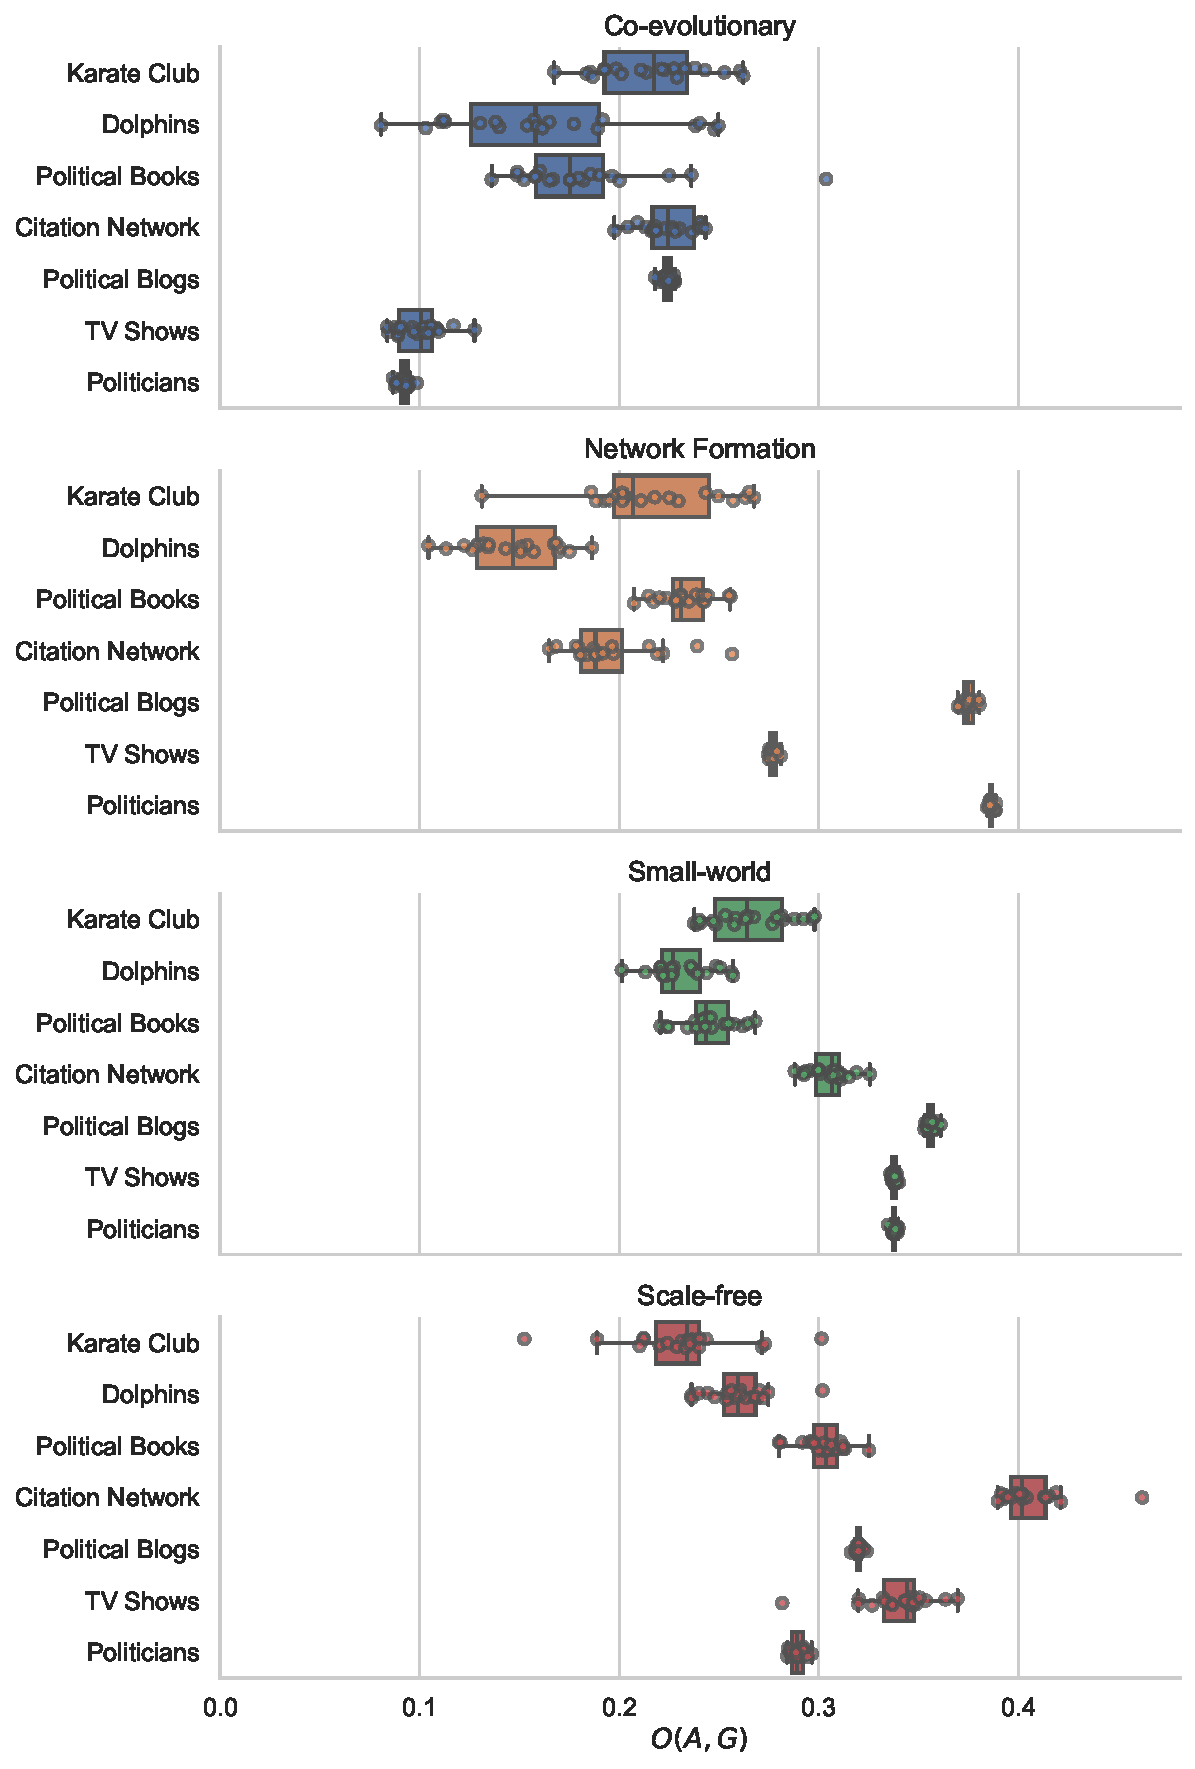
\includegraphics[width=.9\linewidth]{../plots/overall/Model_Evaluation.pdf}
  \caption{Model performance for different networks. The x-axis shows the mean difference between the actual empirical networks and the generated network, $O(A, G)$. The y-axis shows the different empirical networks considered. The colors show different algorithms for generating networks. The dots show the result from individual simulations, while box plots show the median and quartiles of the distribution of values.}
  \label{fig:eval_mean}
\end{figure}

\begin{table}[H]
    \begin{center}
        
    \begin{tabular}{ |p{3cm}||p{1.6cm}|p{1.6cm}|p{1.6cm}|p{1.6cm}|p{1.6cm}|p{1.6cm}|}
        \hline
        \multicolumn{7}{|c|}{Table of network characteristics} \\
        \hline
        \bf{Network} & $N$ & $E$ & $D_{\mu}$ & $D_{\sigma}$ & $\overline{C}$ & $APL$\\
        \hline
        Dolphins   & 62    &159&   5.129&   2.932 &   0.259 & 3.257\\
        Karate Club &34	&78	&4.588&	3.820&	0.571&	2.326\\
        Citation Network & 379 &	914	& 4.823	& 3.927 & 0.741 & 6.052 \\
        TV Shows & 3892 & 17262&8.871 & 12.557 & 0.374&6.324\\
        Political Books &105 &	441	& 8.400 &	5.449 &	0.488 &	3.015\\
        Politicians&  5908 &41729 & 14.126 & 20.096 &	0.385 & 4.628\\
        Political Blogs &	1222 & 16717 & 27.360 & 38.402 & 0.320 & 2.737\\
        \hline
    \end{tabular}
    \end{center}
    \caption{Table of network characteristics. $N$ is the number of nodes, $E$ is the number of edges, $D_{\mu}$ is the mean degree, $D_{\sigma}$ is the standard deviation of the degree distribution, $\overline{C}$ is the average clustering coefficient, and $APL$ is the average path length. }
    \label{table:characteristics}
    \end{table}

\begin{figure}[H]
    \centering
    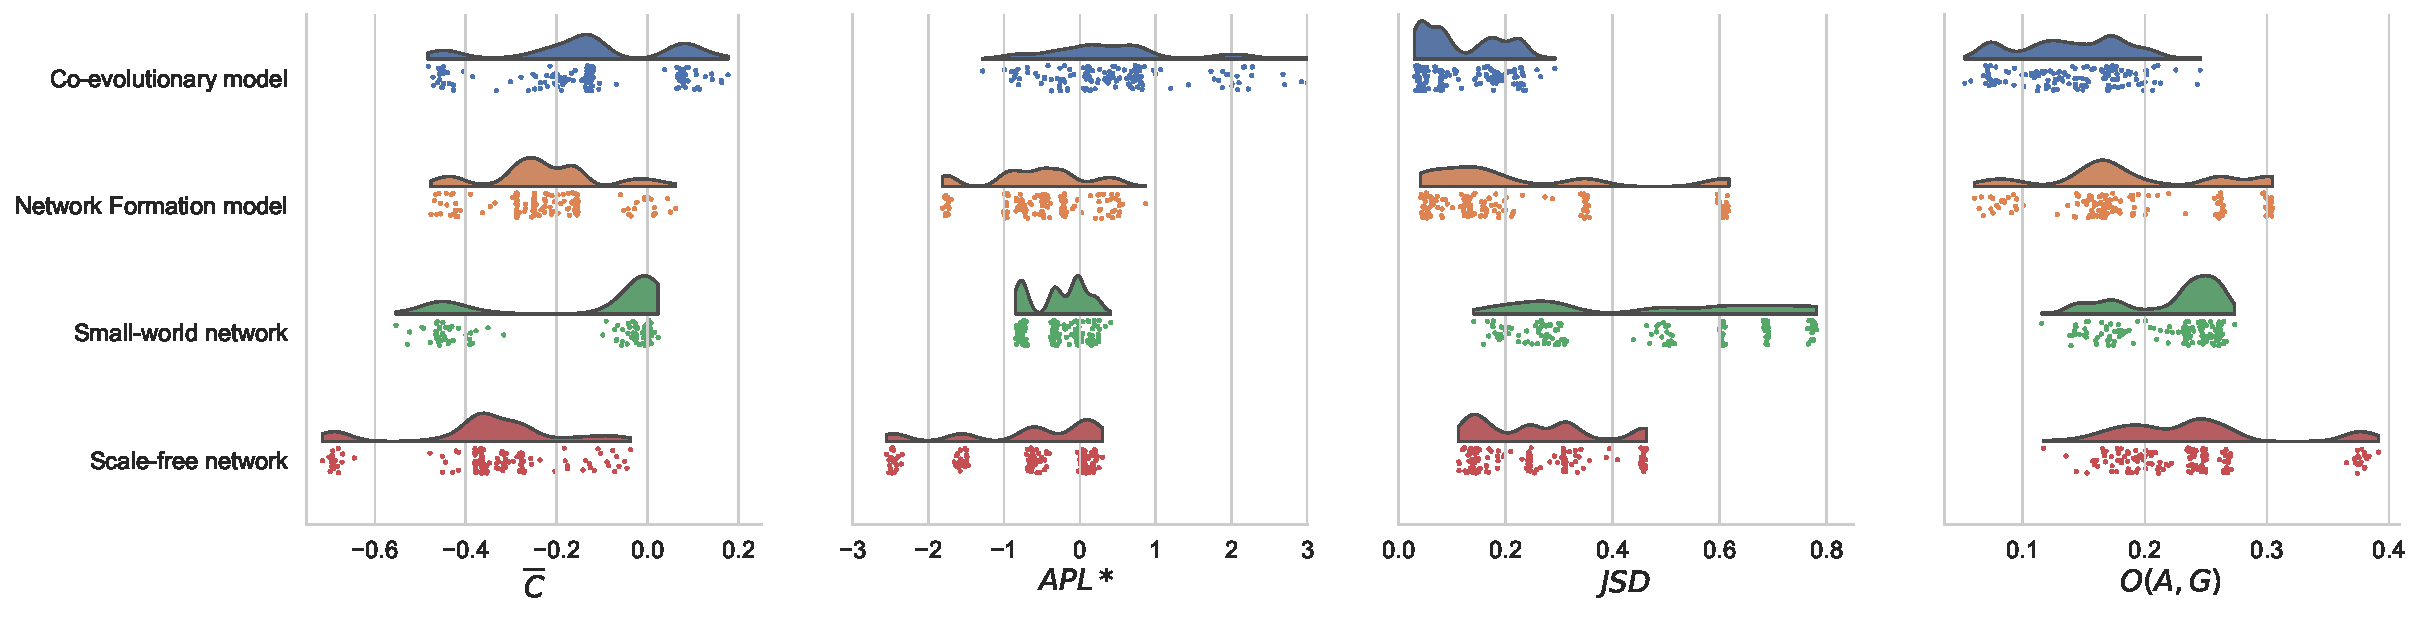
\includegraphics[width=.99\linewidth]{../plots/overall/Model_Evaluation_Overview.pdf}
  \caption{Rain cloud plot of the overall difference in model performance. The plot is divided into four panels. Each panel shows the performance of the four models on different metrics. Each metric is shown on the x-axis. The first two panels show the difference in regard to the average clustering coefficient, $\overline{C}$, and the average path length, $APL*$, respectively. Both were calculated by subtracting the value of the empirical network from the generated networks. The third panel shows the Jensen Shannon Divergence, $JSD$, of the degree distribution from the generated and the empirical networks. Finally, the fourth panel shows the objective function which was minimized during optimization, $O(A,G)$. Performance is indicated by the distance to zero for all metrics. Both the y-axis and the colors show different models of network generation. Dots show the result from individual simulations with the probability density function drawn above the dots.}
  \label{fig:eval_overall}
\end{figure}

\begin{table}[H]
\begin{center}
    
\begin{tabular}{ |p{4.2cm}||p{1cm}|p{0.9cm}|p{1.35cm}|p{1.3cm}|p{1.35cm}|p{1.2cm}|p{0.93cm}|p{0.9cm}|}
    \hline
    \multicolumn{9}{|c|}{Summarized performance for different network formation algorithms} \\
    \hline
    \bf{Model} & $\overline{C}_{MED}$ & $\overline{C}_{IQR}$ & $APL_{MED}$ & $APL_{IQR}$ & $JSD_{MED}$ & $JSD_{IQR}$ & $O_{MED}$ & $O_{IQR}$\\
    \hline
    Scale-free network   & -0.358    & \bf{0.102} &   -0.545	 &   1.555 &   0.245	 & 0.165 & 0.239 & 0.072\\
    Small-world network &   \bf{-0.008}  & 0.390   & \bf{-0.201}	&   \bf{0.699} &   0.499 & 0.418 & 0.236 & 0.071\\
    Network Formation model   &-0.248		 & 0.127	&  -0.498	 & 0.749 &   0.148 & 0.264 & 0.170 & 0.104\\
    Co-evolutionary model & -0.129 & 0.275 & 0.355	 & 0.906 & \bf{0.089} & \bf{0.133} & \bf{0.143} & \bf{0.063} \\
    \hline
\end{tabular}
\end{center}
\caption{Table for the performance of different network formation algorithms. Rows show different network generating models. Columns show the median, $MED$, and inter-quartile range, $IQR$, of the difference between the empirical and the generated networks. For the average clustering coefficient, $\overline{C}$, and the average path length, $APL$, difference was calculated by subtracting the value of the empirical network from the value of the generated network. The Jensen Shannon Divergence, $JSD$, was kept as is, as it already describes the difference between networks. Bold text indicates the value closest to zero in each column.}
\label{table:performance}
\end{table}

\begin{figure}[H]
    \centering
    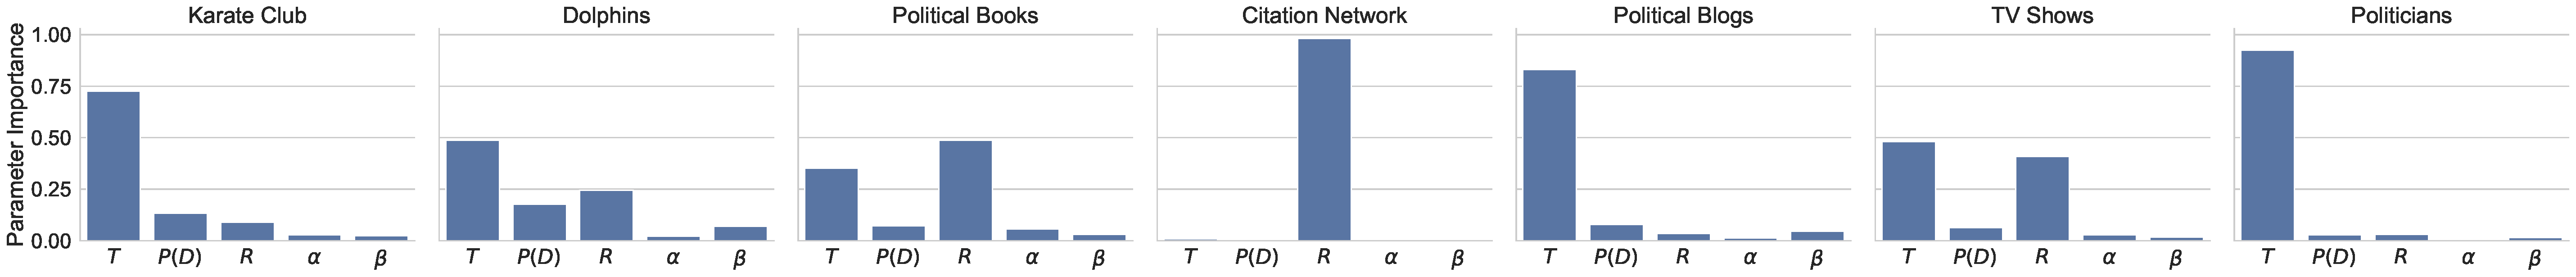
\includegraphics[width=.9\linewidth]{../plots/overall/Parameter_Importance.pdf}
  \caption{Hyperparameter importance. The x-axis shows the different parameters of the Co-evolutionary model. The y-axis shows the fraction of the total variance explained by each parameter i.e. parameter importance. Colors indicate different networks.}
  \label{fig:eval_importance}
\end{figure}

\begin{table}[H]
\begin{center}
    
\begin{tabular}{ |p{3cm}||p{2cm}|p{2cm}|p{2cm}|p{2cm}|p{2cm}|}
    \hline
    \multicolumn{6}{|c|}{Table of best parameter values} \\
    \hline
    \bf{Network} & $R$ & $T$ & $\alpha$ & $\beta$ & $P(D)$\\
    \hline
    Dolphins   & 0.808    &0.288&   0.458&   0.219&   0.865\\
    Karate Club&   0.148  & 0.105   &0.154	&   0.445	&   0.035	\\
    Citation Network   &0.027 & 0.381&  0.222&   0.339&   0.107\\
    TV Show & 0.238 & 0.097 & 0.392 & 0.039 & 0.559 \\
    Political Books &0.001 & 0.588&  0.434&   0.469&   0.249\\
    Politicians&   0.020  & 0.063 &0.197&   0.028&   0.289\\
    Political Blogs & 0.149  & 0.056  &0.046&   0.034&   0.337\\
    \hline
\end{tabular}
\end{center}
\caption{Table of best parameter values for the Co-evolutionary model. Values correspond to the parameter combination, which minimized the objective function the most.}
\label{table:best_params}
\end{table}

\section{Discussion of optimization}
The results from the hyperparameter optimization reiterate that triadic closure works well as a basic generating principle for social networks \cite{jacksonmeeting2007,kossinets_origins_2009,bianconi_triadic_2014}. 
The results reaffirm that small-world networks can generate realistic average clustering coefficients and average path lengths but fail dramatically when it comes to generating realistic degree distributions (see Figure~\ref{fig:eval_overall}) \cite{jacksonmeeting2007}. Triadic closure models are better at generating the patterns in empirical social networks than the most used theoretical models for social networks (see Table~\ref{table:performance}). Models relying on triadic closure can reliably produce realistic degree distributions, as well as high average clustering coefficients. This is the main reason that models using triadic closure reliably outperform small-world and scale-free networks on average. Scale-free networks cannot generate the high average clustering coefficients found in social networks. Interestingly, triadic closure creates more realistic degree distributions than scale-free networks (see Table~\ref{table:performance}). The fact that triadic closure outperforms both small-world and scale-free networks is notable in its own right, as these theoretical networks serve as the basis for many computational models \cite{flache_models_2017, turner_paths_2018}. 

\noindent For the remainder of this discussion, the focus will be on what separates the performance of the two triadic closure models, the Network Formation model and the Co-evolutionary model. 
The Network Formation model is on par with the Co-evolutionary model when the size of the network is small ($N < 400$)(see Figure~\ref{fig:eval_mean}). The only exception to this tendency is the Political Books network, where the Co-evolutionary model is a better model than its Network Formation counterpart.

\subsection{When co-evolution is a better explanation}
As the Co-evolutionary model is a more complicated model, it should be expected that it can fit more complicated patterns. The important question to answer is what specific abilities the model has gained at the cost of higher complexity.
The most plausible answer is that it enables the Co-evolutionary model to systematically generate networks with multiple communities. The notion of a community here refers to a set of nodes that are well-connected locally but not globally \cite{yang2011detecting}. The Co-evolutionary model can generate multiple communities in its generated networks because of the co-evolution between opinion and network dynamics. 
When there is a propensity to delete ties to dissimilar neighbors, $P(D) \gg 0$, communities of like-minded individuals will be created. This is especially the case when new ties are predominantly generated via triadic closure, $R \ll 0.5$, as this will make new connections primarily between agents of the same community. 
If these two conditions are met, the Co-evolutionary model can manipulate how many communities the network contains by adjusting the parameter $T$. 
The lower the value of $T$ is, the less open-minded agents are, as they will have stricter criteria for who to maintain ties with. With lower values of $T$, the resulting network will therefore contain more communities. Notice that for all large networks with more than 1000 nodes, $N > 1000$, the best parameters of the Co-evolutionary model have $P(D) > 0.1$ and $R \ll 0.5$ (see Table~\ref{table:best_params}). The large networks all show low values of $T$, which indicates that the networks consists of many different communities. The large political networks (Politicians and Political blogs) have extremely low values of $T$, which indicate that these political networks are more clearly delineated into multiple communities than the TV Show network. The large networks all have little negative social influence in their best parameters, $\beta < 0.1$. The reason why negative social influence is weak for these networks is most likely to maintain more than two communities in the network. If $\beta \gg 0.1$ and $T \ll 0.5$, the model only creates two communities in its network, as opinions will be pushed to the extreme value of either 1 or -1. 

\subsection{The impact of communities}
It is no coincidence that the Co-evolutionary model performs better than all other models when the networks are large. Large networks very rarely consist of only one community. All members of large networks are unlikely to be equally well-connected to each other. It is far more likely that large networks contain several communities or subgroups, where social agents mostly interact with a small subset of all the agents of the network \cite{backstrom2006group}. 
Although the number of communities can vary greatly, having multiple communities in a network is a feature of most large social networks \cite{backstrom2006group, yang2011detecting}.
This difference in how many communities the models can create can account for the large disparity between the Co-evolutionary model and the Network Formation model. 
The Network Formation model simply doesn't have the ability to generate multiple communities systematically. This will obviously have a large effect on the performance of the model, as having multiple communities will have a strong influence on all the considered network metrics. 

To see the impact of communities on the considered network metrics, we start by considering how having multiple communities changes the average path length of a network. 
All else being equal, a network with more communities will have a greater average path length than a network without multiple communities. 
Communities are very well-connected locally, but not very well-connected globally. 
Few information highways will exist between communities, resulting in a greater average path length than if there had not been multiple communities in the network. 
This is also evident from the results. In five out of the seven networks considered, the average path length is consistent, the average path length of the network generated by the Co-evolutionary model is consistently higher than the average path length of the network generated by the Network Formation model (see Appendix~\ref{appendix:eval_path}).

Having multiple communities will also have a large effect on the degree distribution of a network. When networks consist of multiple communities, the network will tend to have fewer very low degree nodes and fewer very high degree nodes. 
In other words, the network will have less extreme disparity in its degree distribution. 
Extremely high degree nodes become less plausible, simply due to the fact, that an agent is very unlikely to be part of many communities at the same time. 
It will therefore sever connections to more agents than had there not been multiple communities. 
The number of extremely low degree nodes will tend to be low when the network has multiple communities as these communities are locally well-connected. Being part of a tight-knitted community makes it likely that other members of your community will create a connection to you via triadic closure. Therefore, low degree nodes will have more connections within these communities than they would have if there had only been one community. 
These two effects combined will tend to make the degree distribution of the network less scale-free and more log-normal, which is more in line with the degree distribution of most social networks \cite{broido_scale-free_2019}. This is also congruent with the much lower Jensen Shannon Divergence of the Co-evolutionary model, where the large political networks (Political Blogs and Politicians) show large disparities between the Network Formation model and the Co-evolutionary model in Jensen Shannon Divergence of the degree distributions (see Appendix~\ref{appendix:eval_divergence}).

Finally, the clustering coefficient is also affected by the having multiple communities in a network. 
For large networks, one should expect the average clustering coefficient to increase for networks with communities (see Appendix~\ref{appendix:clustering}). 
This is because the communities are well-connected locally, and exhibit very similar features to that of connected caveman networks \cite{watts_networks_1999}. 
Again, the difference between the Network Formation model and the Co-evolutionary model is most vivid for the larger networks of Political Blogs, Politicians and TV Shows (see Appendix~\ref{appendix:eval_clustering}).

\noindent Explaining the difference in results between the two models by the Co-evolutionary model's ability to generate multiple communities is also supported by the fANOVA analysis. 
A recurring theme across all metrics is that the large political networks are the networks where the Co-evolutionary model most clearly outperforms all other models. 
As was stated, these large political networks have very low values of $T$, which indicates that these networks consist of many communities. 
The fANOVA results show that all networks except three have $R$ as their most important parameter. These three exceptions are the two large political networks and the Karate Club network. These networks place an unusual amount of parameter importance on $T$ instead. It is notable in this regard that the other large network, the TV Shows network, also has $T$ as a very important parameter.
Seeing the Karate Club being part of this group of exceptions is is especially interesting since this network is notoriously a polarized network \cite{zachary_information_1977}. What is most notable in the results is that in the large political networks, the parameters that explain the most variance is the variables that govern opinion dynamics and not network dynamics.

\subsection{Including empirical data in agent-based models}
Although the explanation outlined above should be considered highly plausible, it does not exhaust all possible explanations for the underlying difference between the different models. A more complete explanation would be possible by improving how empirical data is integrated with the model. 
For instance, the integration should be improved in regard to the quantity of data, as only seven empirical networks are considered. This limits the certainty with which conclusions can be drawn from the analysis. For instance, controlling for the variable of size was done primarily by including only one network, namely the TV Show network. The TV Show network is of a similar size as the Politicians network and was created using the same method. However, this doesn't control for the variable of size explicitly. This could be done by varying the size of a network by for instance sampling a subset of the nodes of the network. However, it is not clear how such sampling should be done while maintaining the patterns of the original social network. 

The analysis would also be more exhaustive by improving the quality of the data. The empirical validation of the agent-based models provided in this paper compares static snapshots of empirical networks to the final result of a generative model. How well the patterns of the generative process fit with the static empirical networks is only interesting if it lends credence to the idea that the empirical networks could have been generated by the principles of the generative model. 
A better way to test how well the principles of the generative model describe reality would be to not use proxy measures but to study empirical dynamical networks directly. A data-set that included the social connections and the opinions of social agents over time would be invaluable to the field of opinion dynamics. Such a data-set would allow us to gauge more directly how the mechanisms of co-evolution work in real social networks. 
However, this kind of data is of course extremely hard to come by. One of the main reasons that opinions are primarily studied with agent-based models in the first place is that such data-sets are a rarity. Moreover, measuring the opinions of each social agent is a cumbersome process \cite{chartishvili2019approach}. Previous studies have relied on objective demographic measures to calculate similarity \cite{kossinets_origins_2009, bener_empirical_2016}. If one tried instead to gauge opinions, it is unclear how one would get good measures without the inherent problems that come from self-reporting \cite{best2007measuring}. 

Although most researchers lack the high resolution data from dynamical networks, there is still ample possibility to include empirical data in theoretical models. 
The analysis shows that it is possible to use recent insights from data science to not only answer how well models match up with reality, but also why they perform well or not. 
This is possible specifically through the use of frontier methods such as the hyperparameter optimization used here. To the authors' knowledge, the use of a fANOVA to investigate the importance of each parameter has not previously been done with agent-based models.
One can hope that this will inspire future papers to use make use of this method, as it aids the interpretability of the results from hyperparameter optimization considerably. 

\noindent In conclusion, triadic closure alone can generate characteristic patterns from social networks better than small-world and scale-free networks. This strengthens the notion that triadic closure is the basic generating mechanism for social networks \cite{ilany_social_2016,jacksonmeeting2007, jacksonsearch2004}. Moreover, including co-evolutionary mechanisms makes for a much better model of social networks, especially when these networks are large and opinionated. 
The fact that including opinion dynamics substantially improves network dynamical models suggests that there is a clear interdependence between the effects of network and opinion dynamics. We have seen that opinion dynamics can drastically alter the dynamics of networks. We now turn to the other side of this interplay by considering how network dynamics can change opinions.

\part{Co-evolution's effect on opinion dynamics}

To explore the effect of co-evolution, the focus is on how different parameter combinations interact in the Co-evolutionary model with a fixed number of agents. Of special interest is the effect of the parameter $P(D)$, which controls the probability of deleting negative ties. 

\noindent For the following section, all simulations terminate after 10.000 time-steps ($t_{max} = 10.000$), and were made with an initial small-world network with $N=1000$ and $k=7$. 

\noindent To simplify the analysis, the system focuses specifically on the case where opinions are primarily clustered in two groups. As seen in the previous part, this can be achieved by considering appropriate levels of $T$. This simplification was made as it allows for a simpler interpretation of the system. Specifically, it allows for measuring the polarization of each agent simply as the absolute value of their opinion. When only two groups are considered, a consensus is reached when agents cluster around the mean value of 0. Taking the mean of all absolute values of opinions gives a measure of how polarized the system is as a whole. 

\section{Outcome metrics} 
Several outcome metrics are recorded to gauge the effect of each of the model's parameters. Some of these outcome metrics are time-dependent, while others are recorded when the simulation concludes and the system is at its final state. 

\subsection{Time-dependent metrics}
The state of the model is recorded at every 20th time-step.
To track the polarization of opinions over time, the mean and the standard deviation of the absolute value of the opinions of all agents are recorded.
To track the effect of tie-deletion, the cumulative frequency of deleted ties is recorded.
To characterize the network dynamics over time, the average clustering coefficient and the average path length of the network is recorded.
The opinion of every agent is recorded at every 500th time-step. This is done primarily to be able to visualize the trajectory of opinions directly instead of focusing on the absolute value of opinions. 

\subsection{Final state metrics}
At the beginning of each simulation, the initial opinion of every agent, $O_I$, is recorded. At its final state, the final opinion of every agent, $O_F$, is recorded. 
The difference between these two measures is calculated to measure how opinions changed during the simulations. Specifically, the difference between the absolute value of the final and the initial opinion of every agent, $\abs{O_F} - \abs{O_I}$, is calculated. This gives a measure of whether the final opinion of agents is more extreme than their initial opinion. When $\abs{O_F} - \abs{O_I}$ is negative, the initial value of an agent was more extreme than the final opinion of the agent. Similarly, positive values of $\abs{O_F} - \abs{O_I}$ indicate that the opinion of an agent has become more extreme over the course of the simulation. 

\subsection{Correlations}
To measure how much initial opinions are related to the final opinion of agents, the Pearson Correlation Coefficient between the final and the initial opinion of the agents, $\rho_{O_I, O_F}$, is calculated.
Similarly, the Pearson Correlation Coefficient of the average path length and mean of the absolute value of opinions of all agents over time, $\rho_{\abs{O}, APL}$, is calculated. $\rho_{\abs{O}, APL}$ is a measure for how the polarization of the agents correlates with the average distance between agents in the network.

\section{Model parameters}

Only a subset of the possible values for the five parameters of the Co-evolutionary model is considered to make the model computationally tractable. All different possible parameter combinations of this subset are used to make different simulations, resulting in 3.780 different parameter combinations. For each parameter combination, 10 different simulations are made with different random seeds. In total, the Co-evolutionary model is investigated on the basis of 37.800 simulations. The considered parameter values are:

\begin{align*}
    R \in & \{0.1, 0.3, 0.5\} \\
    \alpha \in & \{0.05, 0.10, 0.15, 0.20, 0.25\} \\
    \beta \in & \{0.00, 0.05, 0.10, 0.15, 0.20, 0.25\}\\
    T \in & \{0.6, 0.7, 0.8, 0.9, 1.0, 1.1, 1.2\}\\
    P(D) \in & \{0.0, 0.2, 0.4, 0.6, 0.8, 1.0\}\\
\end{align*}

\noindent Some justification of the different parameters is in order. 
Concerning the power of social influence, it is fair to assume that its power comes from the frequency of social interactions. 
One rarely reaches a perfect compromise when debating other people, which is what $\alpha = 1$ would reflect. It is fair to assume that the parameters controlling social influence should have fairly low values. Specifically for this model, it makes sense to assume that both $\alpha \leq 0.25$ and $\beta \leq 0.25$. Negative social influence is as mentioned less empirically validated than positive social influence \cite{takacs_is_2014, turner_paths_2018}. For this reason, simulations with $\beta = 0$ are also included. 
As mentioned, the considered values of $T$ was specifically chosen to limit the number of clusters in the resulting network. Within this limit, the specific parameter values for $T$ were chosen as they gave the most interesting results in preliminary analyses. For $T > 1.2$, the model more or less always converges to consensus, no matter what the values of all other parameters are. In the same vein, only very few simulations avoid polarization for $T < 0.6$. The parameters of interest are therefore between these two values, where $0.6 \leq T \leq 1.2$. 
Based on the prevalence of triadic closure in empirical social networks \cite{kossinets_origins_2009}, the interesting values of $R$ reflect that at least half of new connections are made via triadic closure, $R \leq 0.5$.
Finally, as co-evolution is one of the main phenomenons of interest here, the whole range of the co-evolutionary force of the probability of tie-deletion, $P(D)$, is studied. Values of interest range from no co-evolution to perfect co-evolution i.e. $0 \leq P(D) \leq 1$.

\section{Results}
The effects of all the different model parameters as well as the correlations of interest outlined previously are all analyzed and reported. However, not all of these results are centered around the main argument of this paper. For this reason, auxiliary visualizations and analyses are reported in the \textit{\nameref{appendix}}.

\subsection{The effect of the different model parameters}
All parameters directly associated with opinion dynamics in the model show clear effects on polarization. Higher values of the threshold, $T$, decrease polarization (see Appendix~\ref{appendix:threshold}). A stronger force of positive social influence, $\alpha$, decreases polarization (see Appendix~\ref{appendix:alpha}). A stronger force of negative social influence, $\beta$, increases polarization (see Appendix~\ref{appendix:beta}).
The drivers of polarization are low values of $T$ and high values of $\beta$. When the value of $T$ is sufficiently low and the value of $\beta$ is sufficiently high, all agents will have more extreme opinions at the end of the simulations than they had in the beginning. Such conditions are both found with $T = 0.6$ and $\beta \geq 0.15$ as well as $T \leq 0.9$ and $\beta = 0.25$. With intermediate values of $\beta$ and $T$, whether the opinions of a simulation become polarized or not is largely dictated by $P(D)$ (see Figure~\ref{fig:radicalization}). 
The results indicate that higher values of $P(D)$ result in lower values of $|O|$ on average. 
The strength of the effect is modulated by how random new connections are made in the network. 
The effect of preventing polarization by deleting negative ties is diminished with increases in $R$ (see Figure~\ref{fig:pd}). Increases in $R$ lead to increased amounts of negative interactions (see Figure~\ref{fig:ntd}). 
When $\beta = 0$, all simulations reach consensus, regardless of all other parameters (see Figure~\ref{fig:radicalization}). Notably, increasing the probability of negative tie-deletion has no effect on polarization when $\beta = 0$ (see Figure~\ref{fig:pd_no_negative}). 
When $P(D) = 0$, $T \leq 1.0$ and $\beta > 0$, the network always polarizes (see Figure~\ref{fig:radicalization}).

\begin{figure}[H]
    \centering
    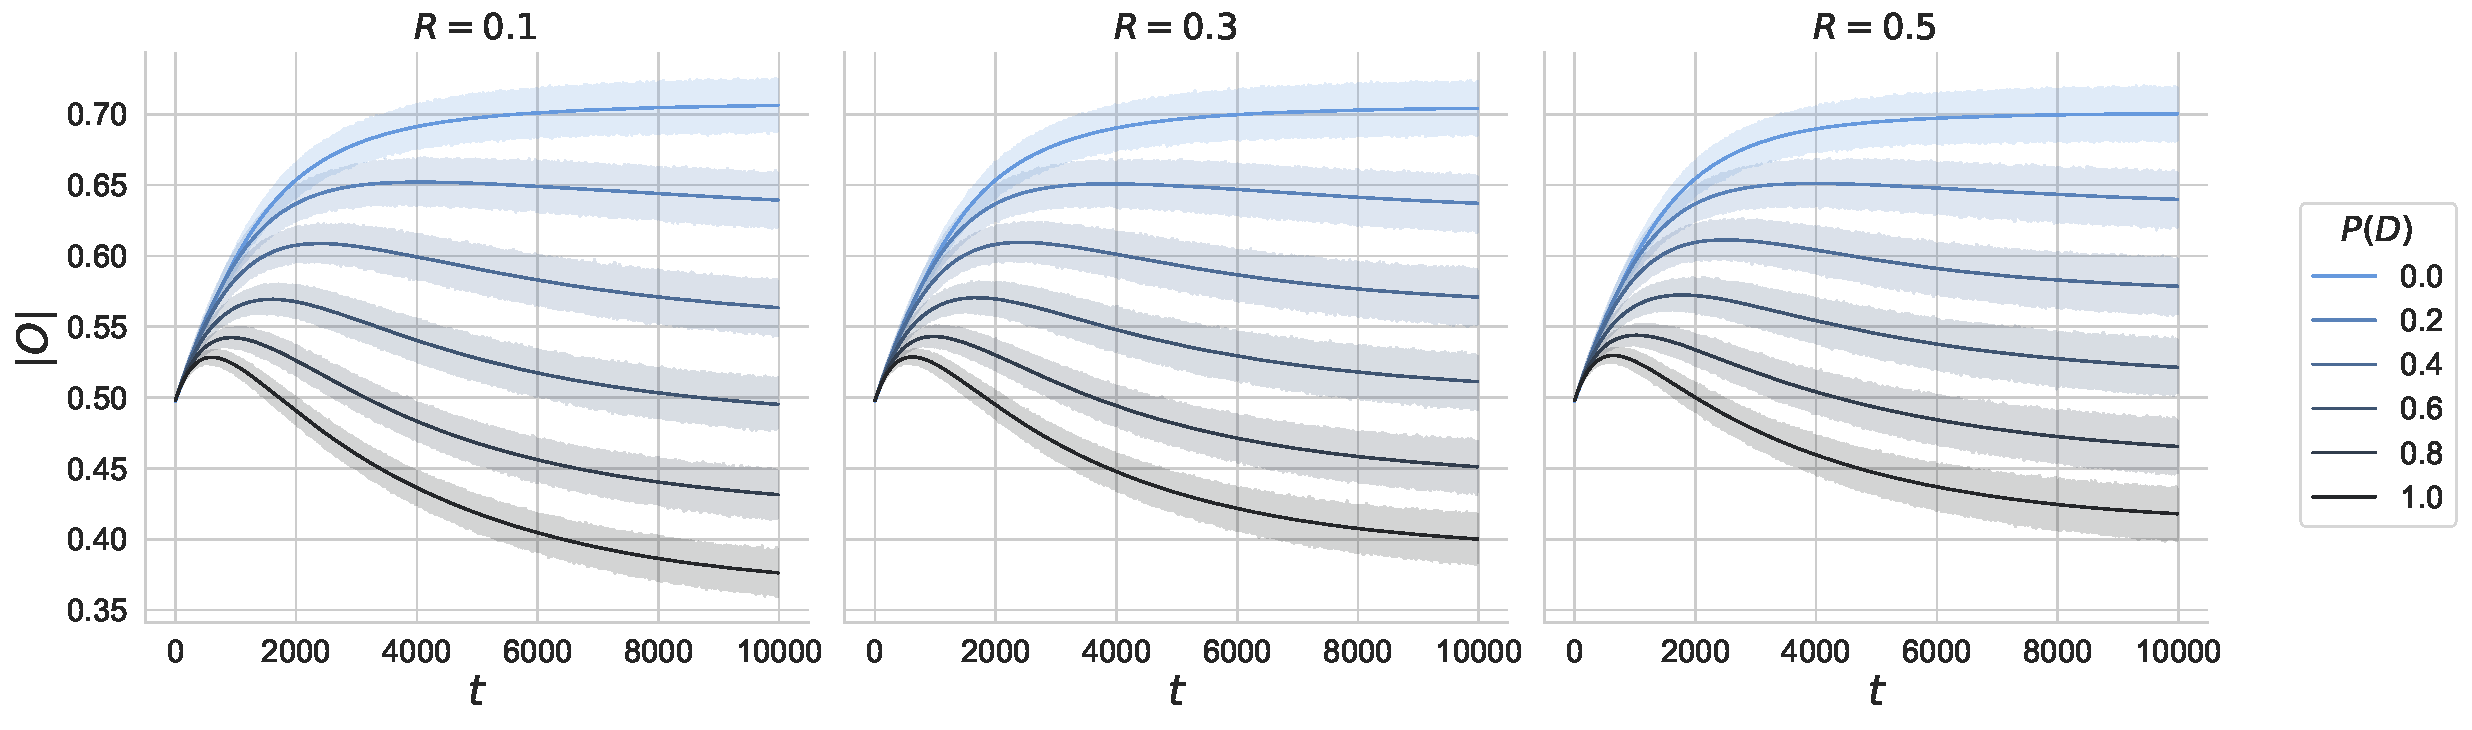
\includegraphics[width=.99\linewidth]{../plots/overall/Absolute_Opinion_Tie_Dissolution.pdf}
  \caption{The effect of tie-deletion on polarization over time. The x-axis shows the time-steps, $t$, and the y-axis shows the absolute value of the opinions of agents, $\abs{O}$. Colors indicate different probabilities of tie-deletion of dissimilar agents. Lines indicate the mean value of each time-step, aggregated over all parameters excluding the probability of tie-deletion, $P(D)$, and randomness, $R$. Shaded regions show the 95\% confidence intervals. The three different panels show simulations with different propensities for generating new ties via triadic closure rather than randomly, $R$.}
  \label{fig:pd}
\end{figure}

\begin{figure}[H]
    \centering
    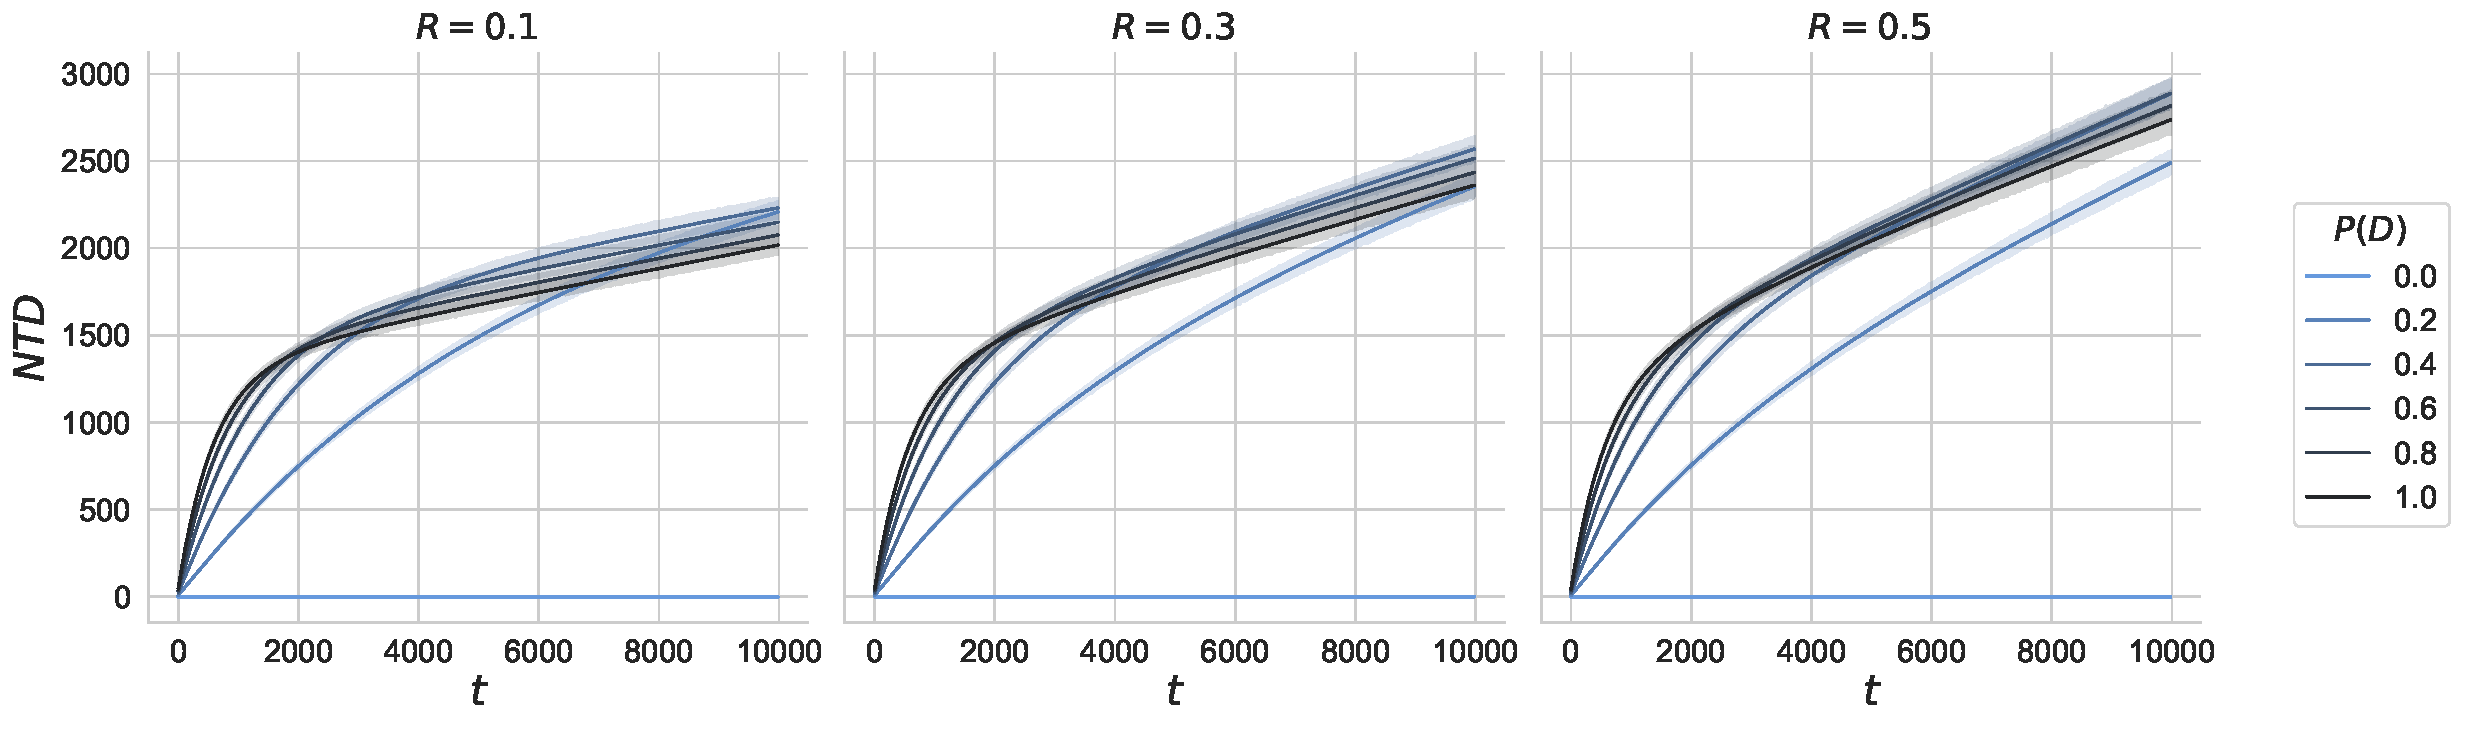
\includegraphics[width=.99\linewidth]{../plots/overall/Negative_Tie_Deleted.pdf}
  \caption{Cumulative frequency of negative ties deleted. The x-axis shows the time-steps, $t$, and the y-axis shows the average cumulative frequency of deleted ties, $NTD$. Colors indicate different probabilities of tie-deletion of dissimilar agents, $P(D)$. Lines indicate the mean value of each time-step, aggregated over all parameters excluding the probability of tie-deletion, $P(D)$, and randomness, $R$. Shaded regions are the 95\% confidence intervals. The three different plots show the different values of the probability of new connections being generated randomly, $R$. Notice that when $P(D) = 0$, no ties are deleted, which results in a bright blue line on the X-axis on all of the plots.}
  \label{fig:ntd}
\end{figure}

\begin{figure}[H]
    \centering
    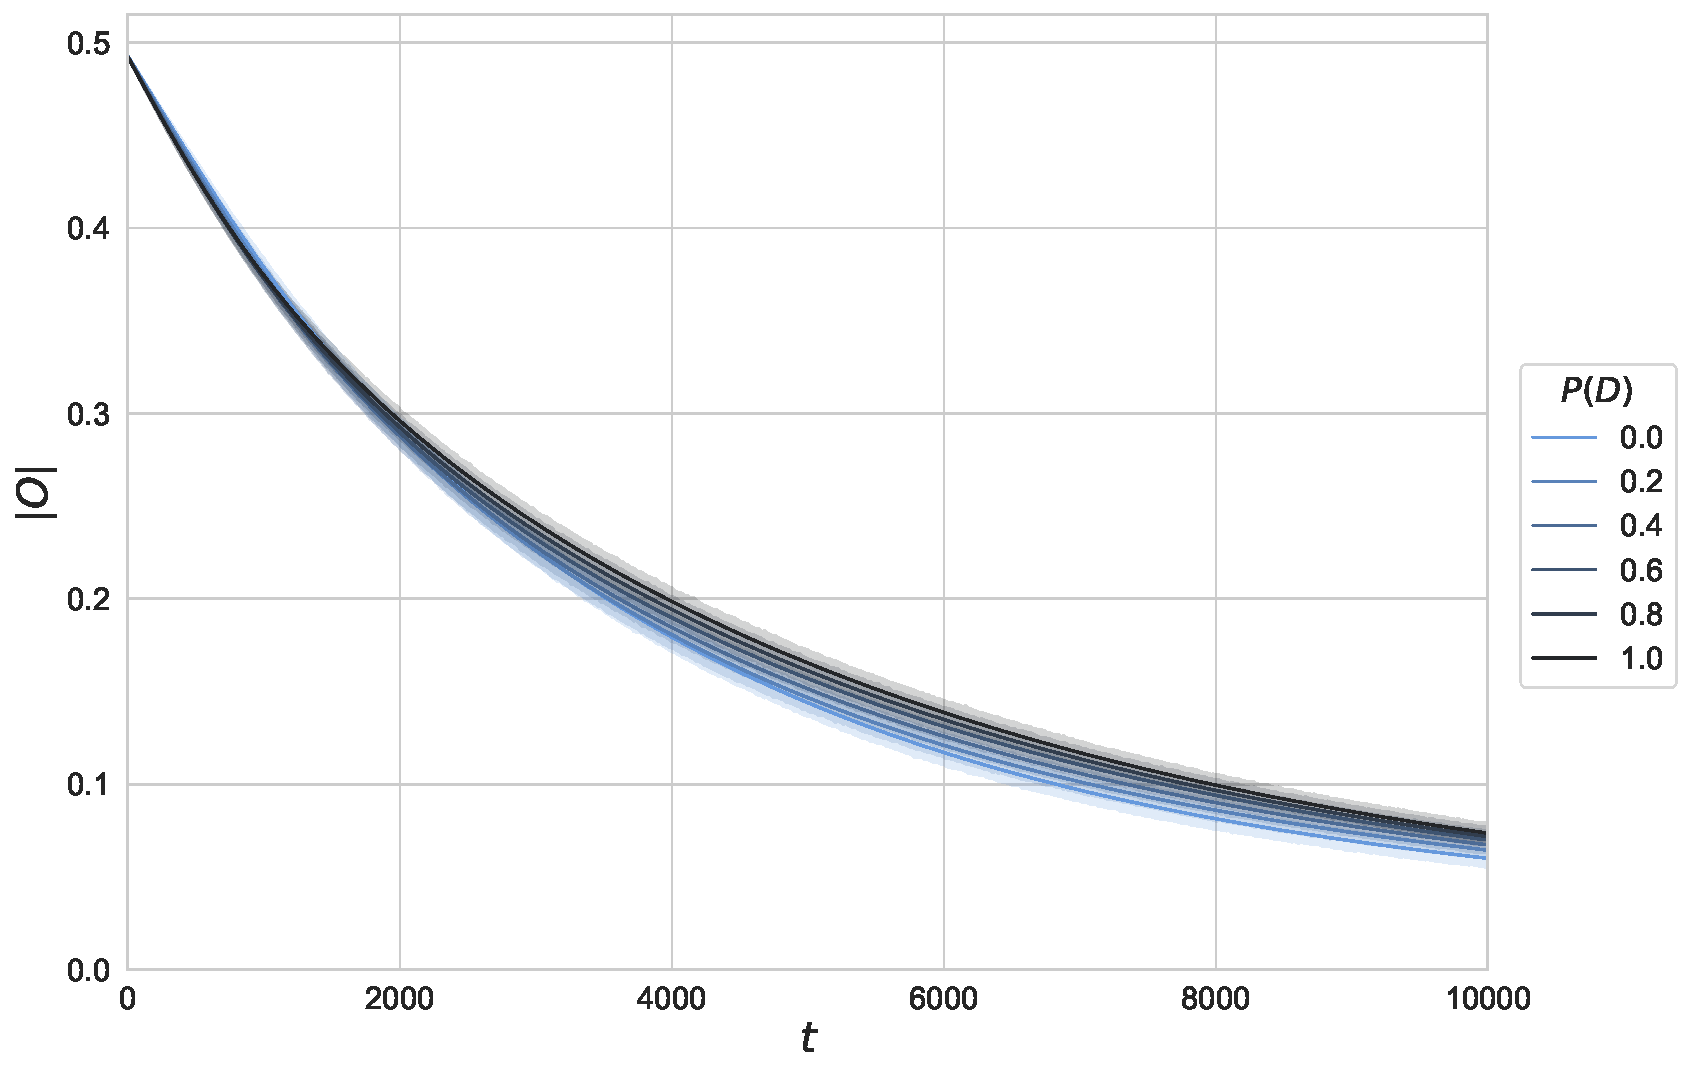
\includegraphics[width=.99\linewidth]{../plots/overall/Absolute_Opinion_Tie_Deletion_Without_Negative.pdf}
  \caption{The effect of negative tie-deletion without negative social influence. The x-axis shows the time-steps, $t$, and the y-axis shows the absolute value of the opinions of agents, $\abs{O}$. Colors indicate different probabilities of tie-deletion of dissimilar agents, $P(D)$. Lines indicate the mean value of each time-step, aggregated over all parameters with $\beta = 0$, excluding the probability of tie-deletion, $P(D)$. Shaded regions show the 95\% confidence intervals.}
  \label{fig:pd_no_negative}
\end{figure}

\begin{figure}[H]
    \centering
    \includegraphics[width=.99\linewidth]{../plots/overall/Radicalization.pdf}
  \caption{Distribution of opinion changes across different conditions. Rows display different values of thresholds, $T$, and columns indicate different values of negative social influence, $\beta$. Different colors show different values of the probability of tie-deletion, $P(D)$. The x-axis shows the difference between the absolute value of the final and initial opinions of agents, $\abs{O_F} - \abs{O_I}$. When this value is positive, the final opinion of agents is more extreme than the initial opinion of agents. When this value is negative, the final opinion of agents is less extreme than their initial opinion. Y-axis shows the percent of values within each bin. }
  \label{fig:radicalization}
\end{figure}

\subsection{Correlations}
The correlation between the absolute value of opinions and the average path length, $\rho_{|O|, APL}$ is largely dictated by the probability of tie-deletion, $P(D)$ and how random new connections are, $R$. For simulations with $P(D) \geq 0.6$ and $R \geq 0.3$, most simulations show high positive correlation coefficients. When $P(D) = 0$, there is no consistent correlation between the two variables (see Figure~\ref{fig:corr_abs_path}). 

\begin{figure}[H]
    \centering
    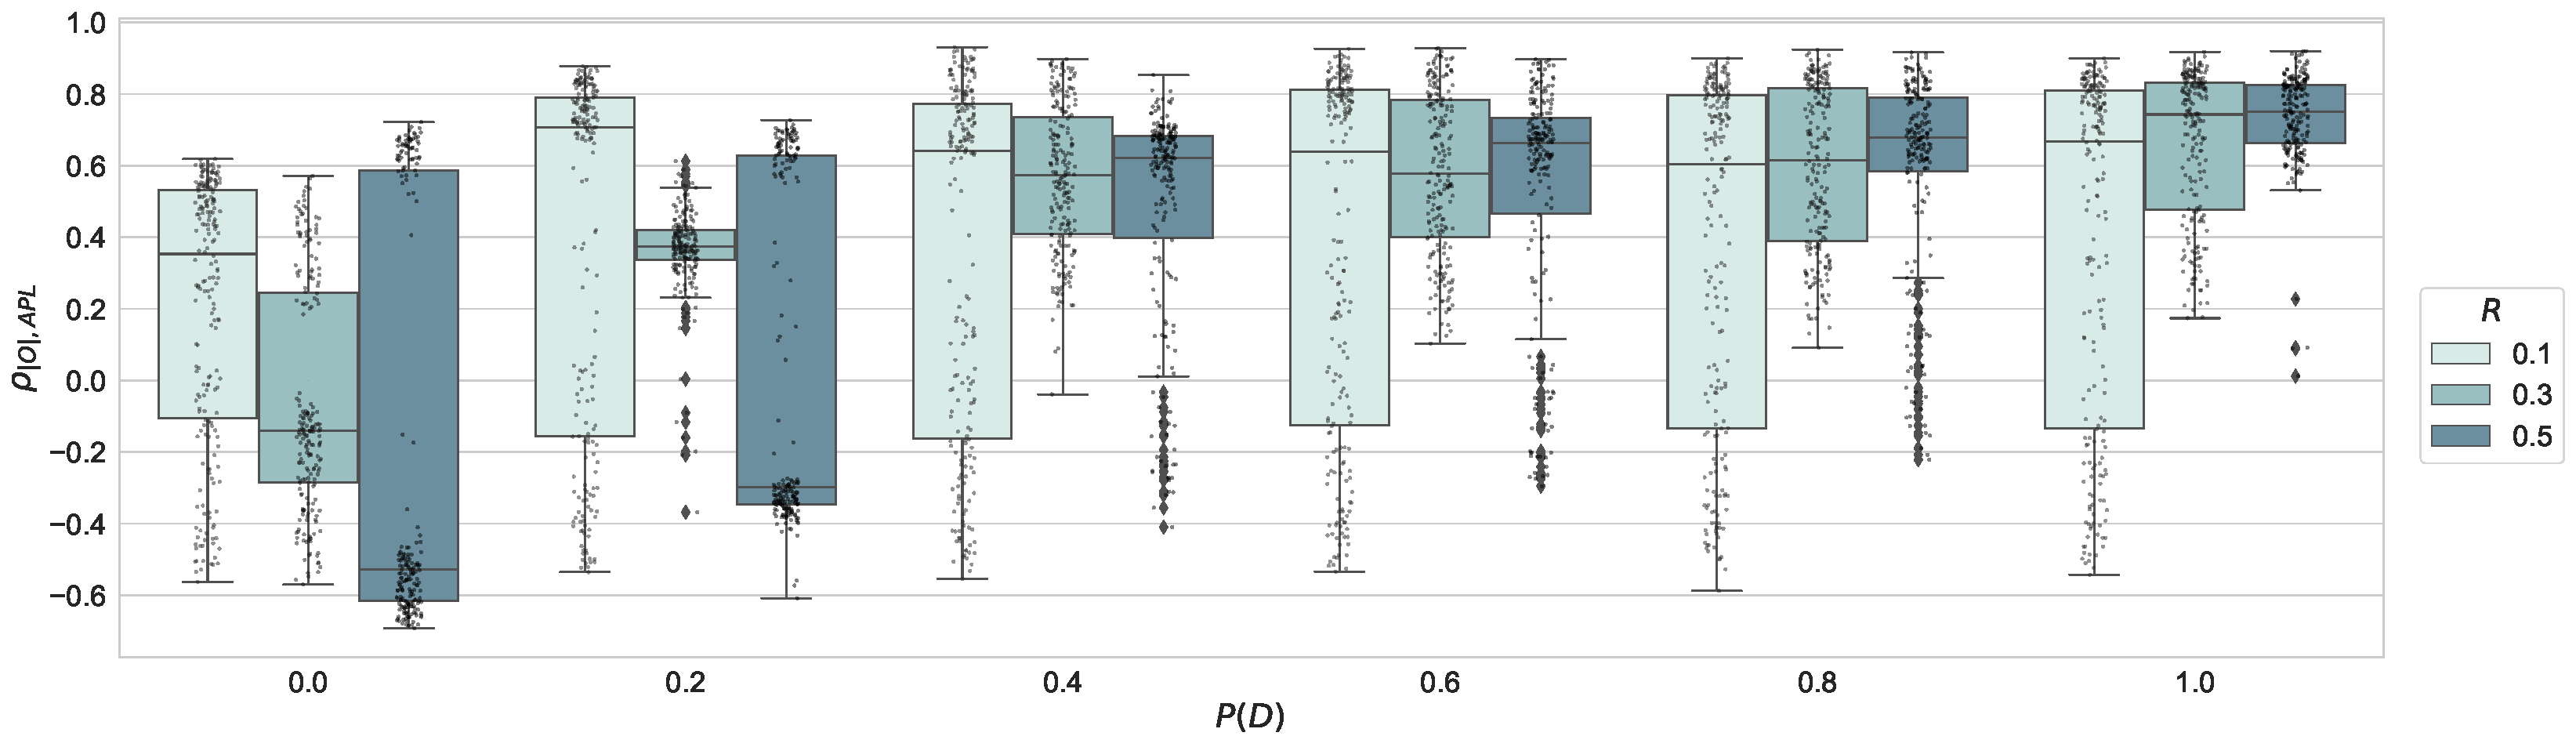
\includegraphics[width=.99\linewidth]{../plots/overall/Tie_Dissolution_Correlations_Boxplot_Full.pdf}
  \caption{Correlations between the mean absolute opinion and average path length. The x-axis shows different values of the probability of deleting negative ties, $P(D)$. The Pearson Correlation Coefficient between the mean of the absolute value of opinions and the estimated average path length, $\rho_{\abs{O}, APL}$ is shown on the y-axis. Boxes indicate the quartiles and whiskers indicate the 1.5 of the inter-quartile range outside of the quartiles. Points outside this range are depicted as diamonds. Smaller dark dots show the correlation coefficient for individual simulations.}
  \label{fig:corr_abs_path}
\end{figure}

\section{Discussion}

\subsection{Reiterating previous literature}
The observed effect of positive social influence, $\alpha$, negative social influence, $\beta$, and the threshold, $T$, are intuitive and in line with previous research on similar models \cite{flache_models_2017}.  When $\alpha$ is high, there is a stronger force pulling the opinion of agents closer together. Higher values of $\alpha$ therefore results in lower values of polarization (see Appendix~\ref{appendix:alpha}). 
The effect of $\alpha$ is small in comparison to the effect of $\beta$ and $T$ (see Appendix~\ref{appendix:threshold},~\ref{appendix:beta}).
When $\beta = 0$, all simulations reach a consensus (see Figure~\ref{fig:pd_no_negative}). When $\beta$ is large, almost all simulations polarize (see Figure~\ref{fig:radicalization}). This is partly because it is a stronger force than $\alpha$ in how it is operationalized.  The effect of pushing and pulling opinions is defined as being proportional to the distance between agents. 
By definition, agents that are pushed away from each other are further apart than agents that are pulling each other's opinions closer together. In this sense, $\beta$ is a stronger force than $\alpha$. Only in aggregate can the effect of $\alpha$ become stronger than the effect of $\beta$. This is only possible when the number of positive interactions is much higher than the number of negative interactions. The effect of $T$ should therefore not be surprising. With larger values of $T$, agents are more open-minded in the sense that they can cooperate with more agents, and will therefore have more positive rather than negative interactions. To see this, notice that if an agent has an opinion of 0 and $T\geq1$, this agent will not be able to have any negative interactions in this model. The opposite effect is witnessed when $T$ is low. When $T$ is low, the subset of agents that any agent can cooperate with is limited, which makes negative interactions more plausible.
\subsection{The importance of co-evolution}
As mentioned in the \textit{\nameref{introduction}}, previous models have primarily focused on studying systems of static networks.
The results show the consequences of this assumption. When the network does not co-evolve and there is some negative social influence in the system, $P(D) = 0$ and $\beta > 0$, the network always polarizes (see Figure~\ref{fig:radicalization}).
This is not the case when the network is dynamic and co-evolves, which can often prevent negative social influence from causing polarization in the network (see Figure~\ref{fig:pd}).
This in and of itself shows that the co-evolution of network and opinion dynamics is a vital piece of the puzzle of polarization. 

\subsection{Tie-deletion can prevent polarization}
One of our main findings is that higher probabilities of tie-deletion can prevent polarization. This is especially the case when new ties are created via triadic closure and not randomly (see Figure~\ref{fig:pd}). The reason for this is that the negative tie-deletion makes the network assort based on opinions. In other words, it happens because of the link between distance in similarity and distance in the network. Recall that this link was a robust finding for empirical social networks (see Figure~\ref{fig:distance_similarity}). Deleting negative ties will cause fewer negative social interactions, which limits the effect of $\beta$. 
As such, deleting negative ties is important in its own right because it deletes ties that would otherwise cause further polarization. But because the system is positively assorted based on similarity, the effect of tie-deletion interacts with how random new ties are created (see Figure~\ref{fig:ntd}). When agents assort based on opinions, the heuristic that "a friend of a friend is also a friend" is very likely true. Triadic closure will result in even more positive interactions when distance in the social network is highly indicative of distance in similarity \cite{kossinets_origins_2009}. As such, new ties created randomly rather than via triadic closure will tend to connect more dissimilar agents. In other words, increasing randomness decreases assortment, which leads to more negative encounters (see Figure~\ref{fig:ntd}). This also echoes the finding from the opinion dynamics literature stating that when new connections are made randomly, opinions will tend to polarize rapidly when they include negative influence \cite{flache_why_2006,flache_small_2011,turner_paths_2018}. Here it is shown that a plausible explanation for this finding is that social networks are assorted based on opinions. By increasing how random new connections are, one increases the probability of having negative interactions. 

\noindent Positive assortment of opinions is also closely linked to why there is a strong positive correlation between the absolute value of opinions and the average path length, $\rho_{\abs{O},APL}$, when negative ties are deleted and when new connections are made more randomly. As the network is co-evolutionary, changes in the network will reflect changes in opinions. The strong positive correlation between the absolute value of opinions and the average path length, $\rho_{\abs{O},APL}$, suggests that when opinions polarize, so does the network (see Figure~\ref{fig:corr_abs_path}).
Importantly, this only happens when negative ties are deleted. When $P(D) \gg 0$, negative ties will tend to be deleted when the opinions of agents polarize. Because of the positive assortment in the system, agents that have dissimilar opinions will tend to be further away from each other in the network. As such, long-range ties in particular will suffer when opinions polarize. This will make social ties that connect distant parts of the network much less likely, which increases the average path length substantially. When the network depolarizes, the opposite happens. Some long-range ties will be made randomly, and because the network is depolarized, these connections most likely stay intact. This will make further long-range connections more probable, as the two clusters can connect via triadic closure. This is the reason that the correlation increases as the value of $R$ increases. 

\subsection{Investigating representative simulations}
The results that have been presented and discussed previously have all been made based on averages of several simulations. Although such averages are well-suited to diagnose the general tendencies of such a system, some intricacies can be lost in averages. Often a more detailed look at representative simulations is fruitful for understanding the system's behavior \cite{turner_paths_2018}. Focusing on a subset of simulations makes it possible to visualize the raw trajectories of opinions and networks simultaneously (see Figure~\ref{fig:lineplot}, ~\ref{fig:networks}). By taking a closer look at representative simulations, it becomes easier to understand how tie-deletion might prevent polarization. To this end, a sharper focus is made on some of the conditions where tie-deletion and triadic closure is the difference between polarization and consensus. The representative conditions investigated in the following section are simulations where the threshold is not large or small, $T = 0.9$, there is some negative social influence, $\beta = 0.2$, and some positive social influence, $\alpha = 0.2$. This combination of parameters only avoids polarization when $P(D) = 1$ for the reasons highlighted in the previous section (see Figure~\ref{fig:radicalization}). 

\begin{figure}[H]
    \centering
    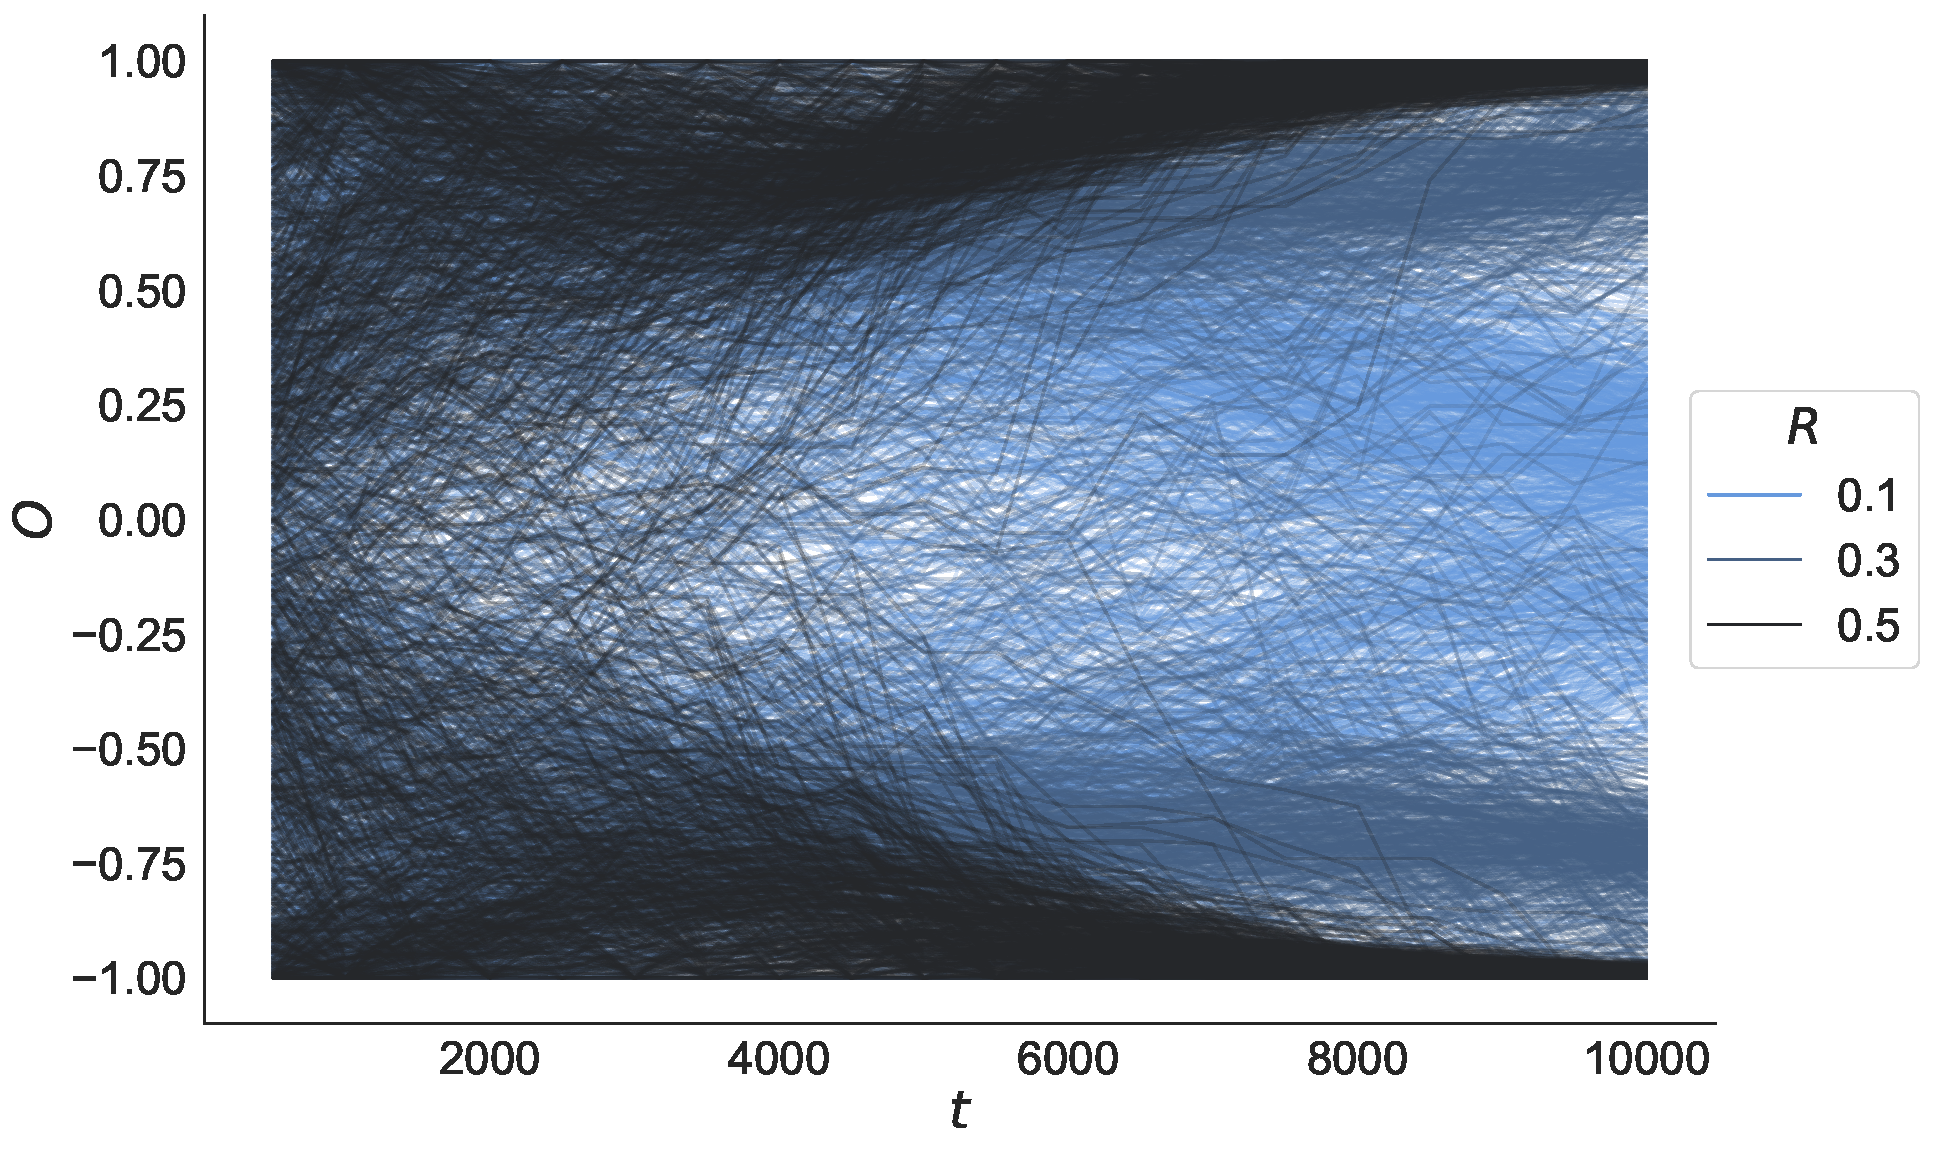
\includegraphics[width=.8\linewidth]{../plots/example/Lineplot_Over_Time.pdf}
  \caption{Lineplot of opinions over time. The x-axis shows time-steps of the simulation, the y-axis shows the opinion of agents in the simulation. Colors show different values of $R$. All simulations were generated with the parameter values of $T = 0.9$, $\alpha = 0.2$, $\beta = 0.2$, $P(D) = 1$ and with the same random seed.}
  \label{fig:lineplot}
\end{figure}

\noindent In these representative conditions, the randomness of new connections, $R$, plays a vital role in whether opinions polarize or not. This can be seen in the stark difference between the trajectories of opinions for different levels of $R$ (see Figure~\ref{fig:lineplot}). Only the simulation with $R=0.1$ avoids polarization. Additionally, when $R=0.5$, the polarization is much faster than when $R=0.3$. For all the representative simulations, there is a strong connection between the average path length of the network and the polarization of opinions (see Figure~\ref{fig:example_abs_opinion}, ~\ref{fig:example_path}). As mentioned, the mechanism that links these two variables is positive assortment. This can be seen by inspecting the opinions of the agents in the network directly. After only 2000 time-steps, there is a clear gradient in the opinion of the agents in the networks, represented in the visualizations as colors (see Figure~\ref{fig:networks}). This is the result of positive assortment. Positive assortment is achieved directly by negative tie-deletion in this model. Additionally, positive assortment is increased indirectly by triadic closure. This is exactly the kind of mechanism described in the literature as structural homophily \cite{asikainen_cumulative_2020,peixoto_disentangling_2022}. This also goes to show that tie-deletion is not necessarily an important mechanism in itself. Rather, it is important because it increases positive assortment. Presumably, any mechanism that will increase positive assortment in these kinds of models will decrease polarization. This point is also strengthened by the difference between the simulations considered here. The reason why the simulations with $R > 0.1$ polarize is that increasing randomness decreases positive assortment. Counter-intuitively, tie deletion in combination with triadic closure can prevent polarization because it isolates groups, not despite it. 

\begin{figure}[H]
    \centering
    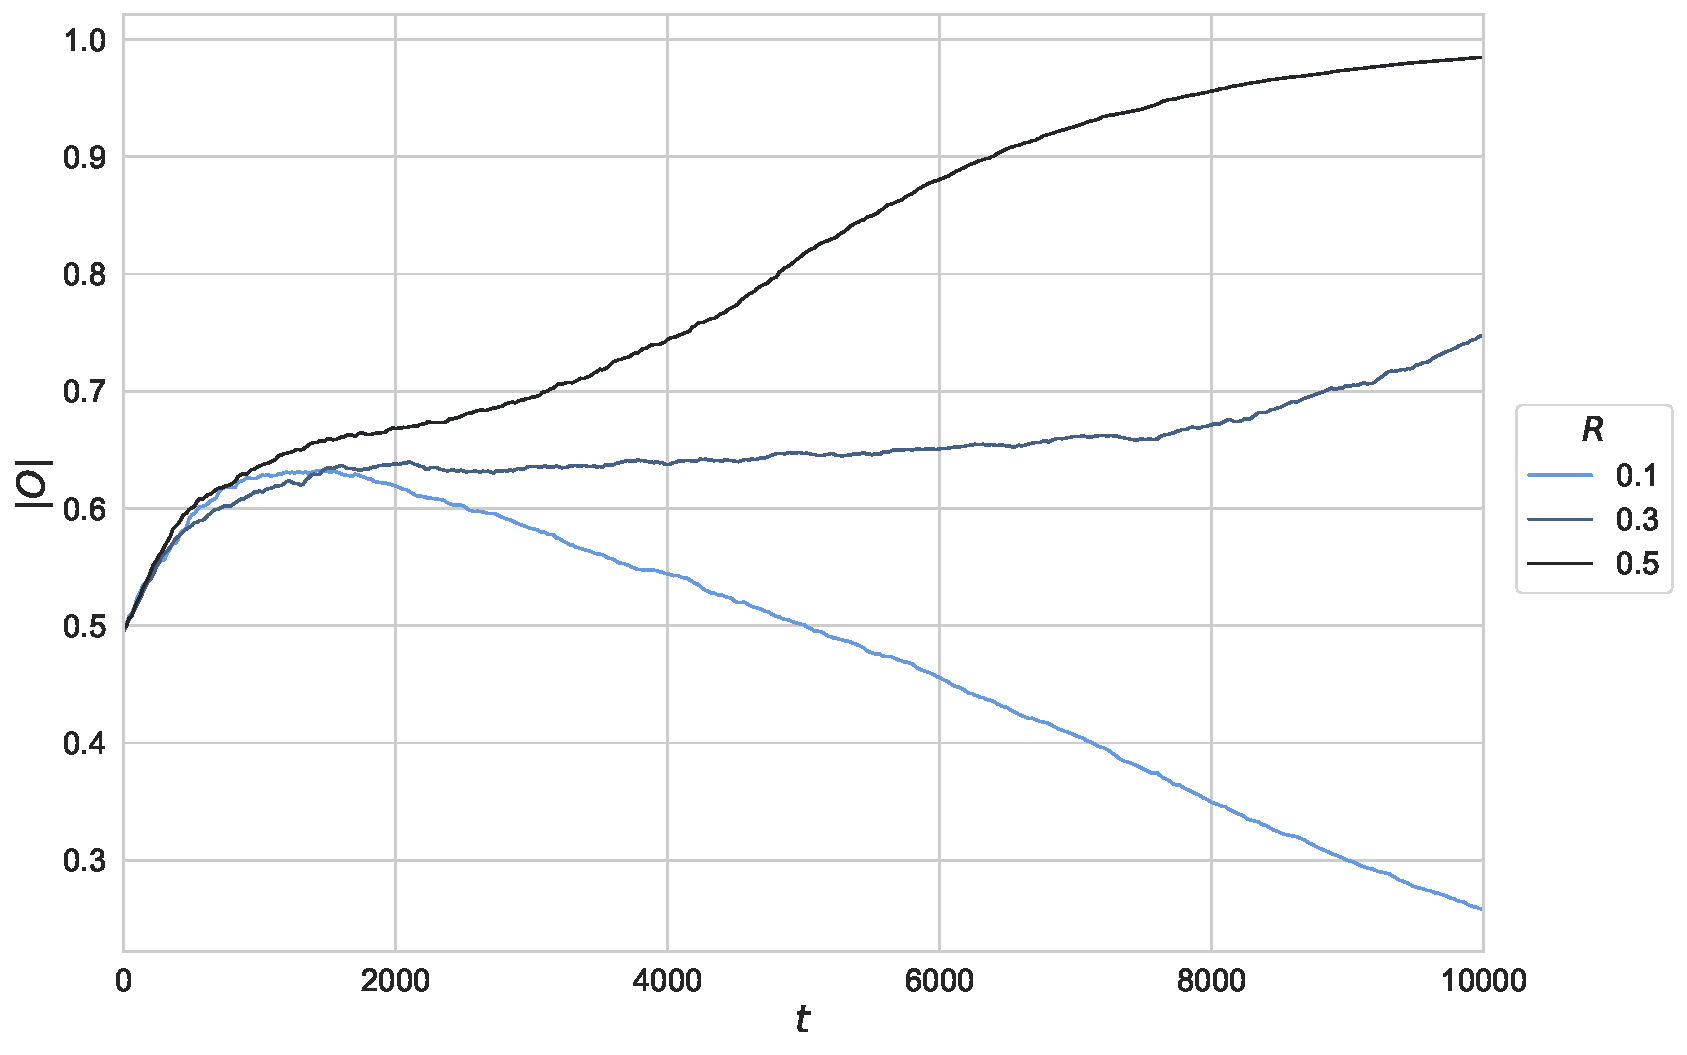
\includegraphics[width=.7\linewidth]{../plots/example/Example_Absolute_Opinion.pdf}
  \caption{Absolute opinions of representative simulations over time. The x-axis shows time-steps, and the y-axis shows the absolute opinion of agents. Colors indicate different levels of randomness. Lines show single simulations over time that were simulated using the same random seed. These simulations had parameter values of $T = 0.9$, $\alpha = 0.2$, $\beta = 0.2$ and $P(D) = 1$.}
  \label{fig:example_abs_opinion}
\end{figure}

\begin{figure}[H]
    \centering
    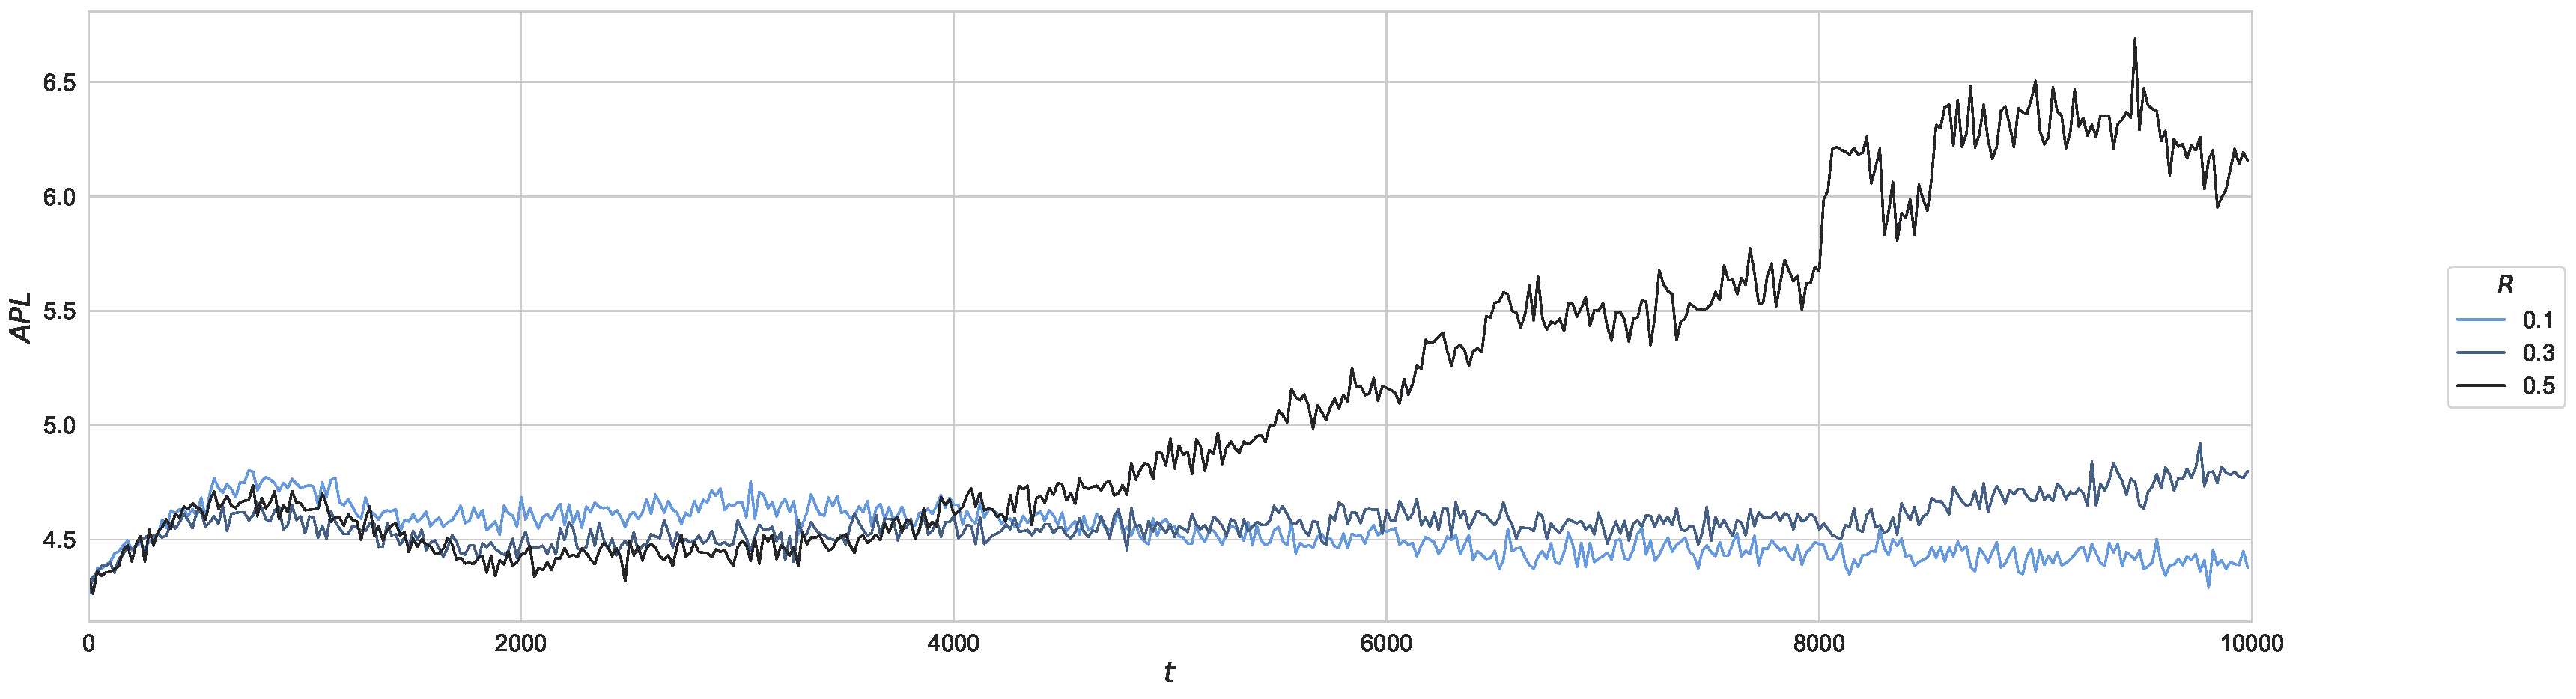
\includegraphics[width=.7\linewidth]{../plots/example/Example_Average_Path_Length.pdf}
  \caption{Average path length of representative simulations over time. The x-axis shows time-steps, and the y-axis shows the average path length of the network. Colors indicate different levels of randomness. Lines show single simulations over time that were simulated using the same random seed. These simulations had parameter values of $T = 0.9$, $\alpha = 0.2$, $\beta = 0.2$ and $P(D) = 1$.}
  \label{fig:example_path}
\end{figure}


\newpage
\begin{center} 
    \begin{figure}[H]
        \centering
    \begin{tabular}{ccc} 
        $R = 0.1$ & $R = 0.3$ & $R = 0.5$ \\
    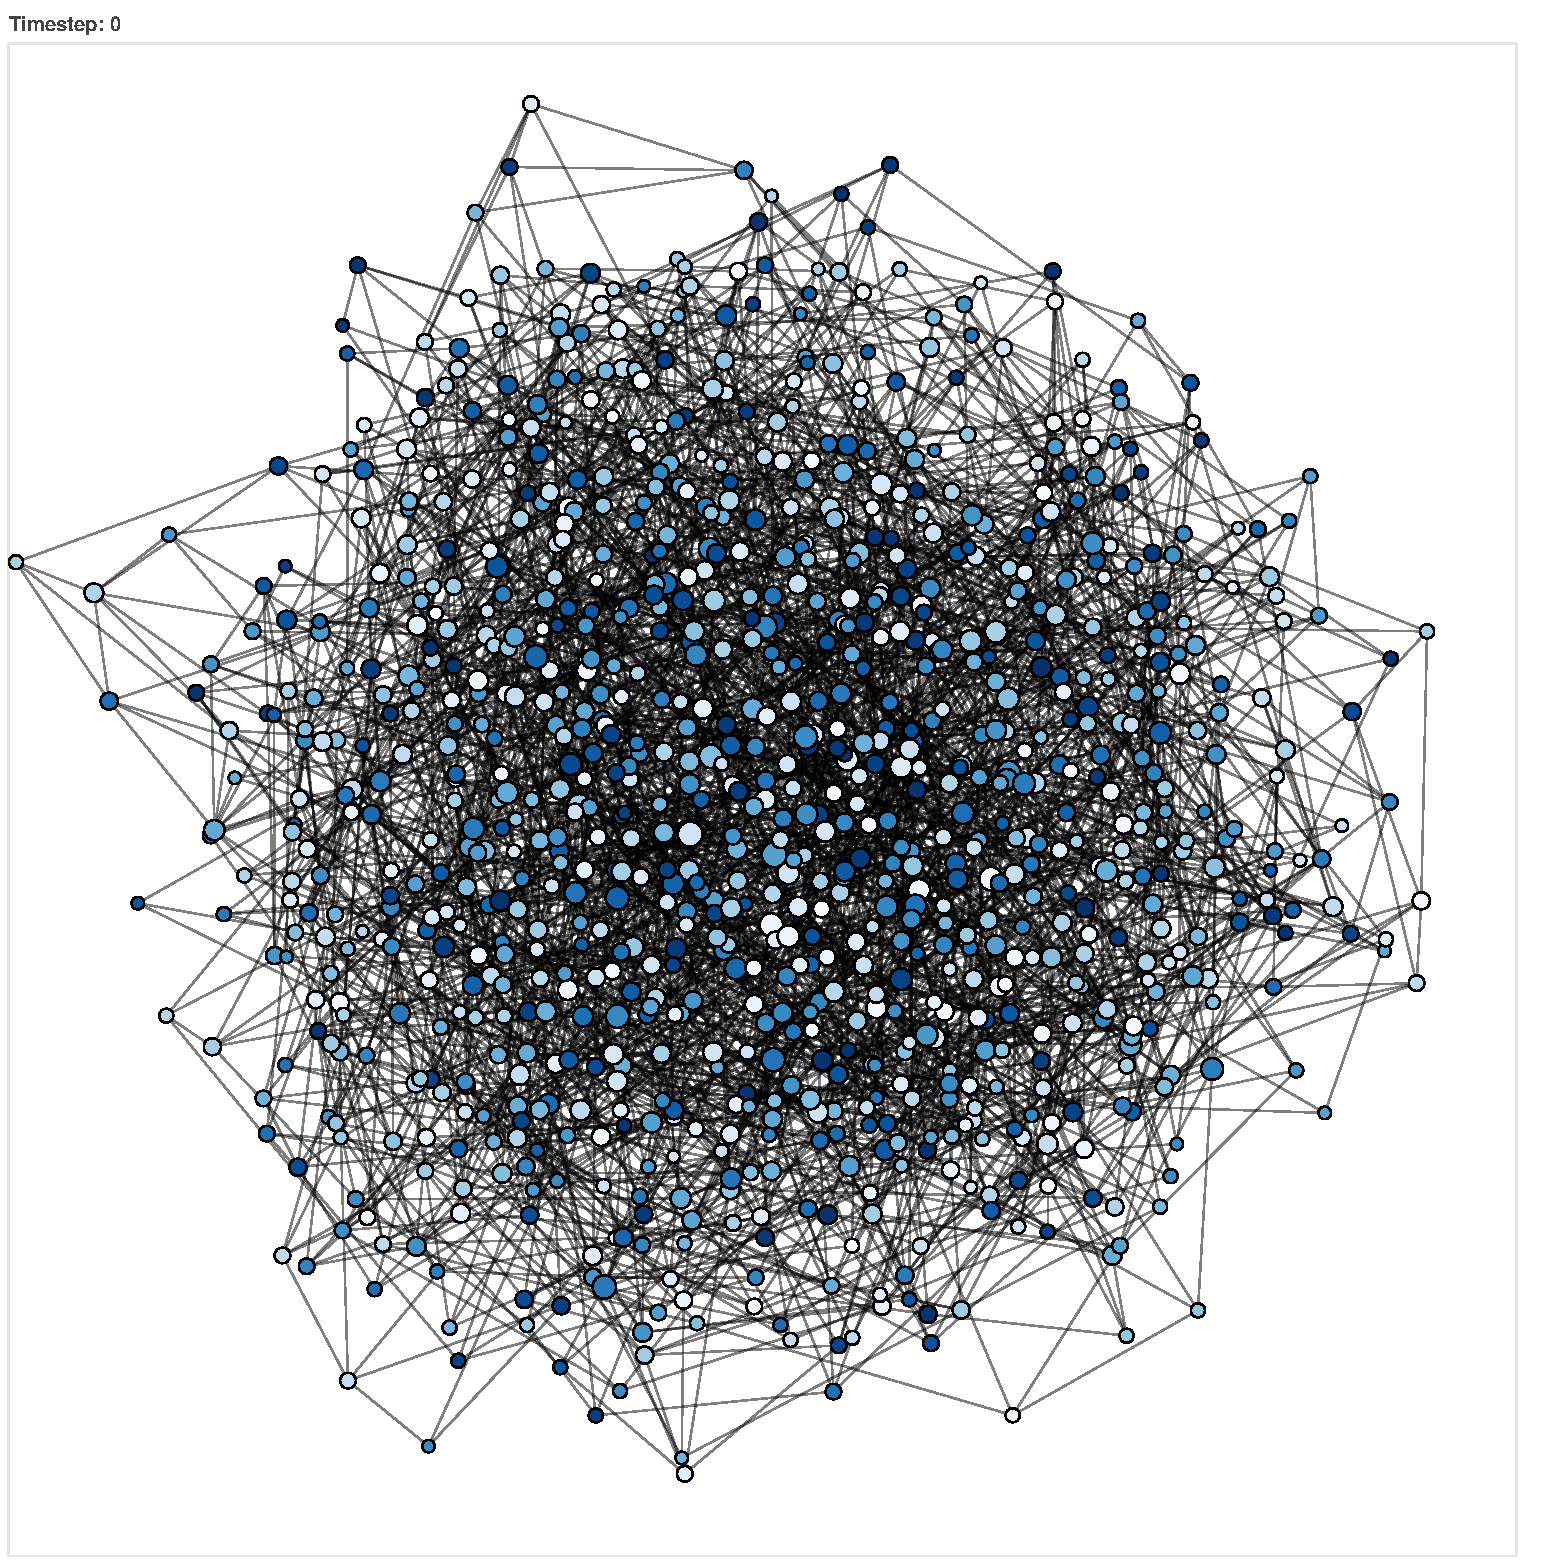
\includegraphics[width=.15\linewidth]{../plots/networks/network_example_R0.1_0.pdf} & 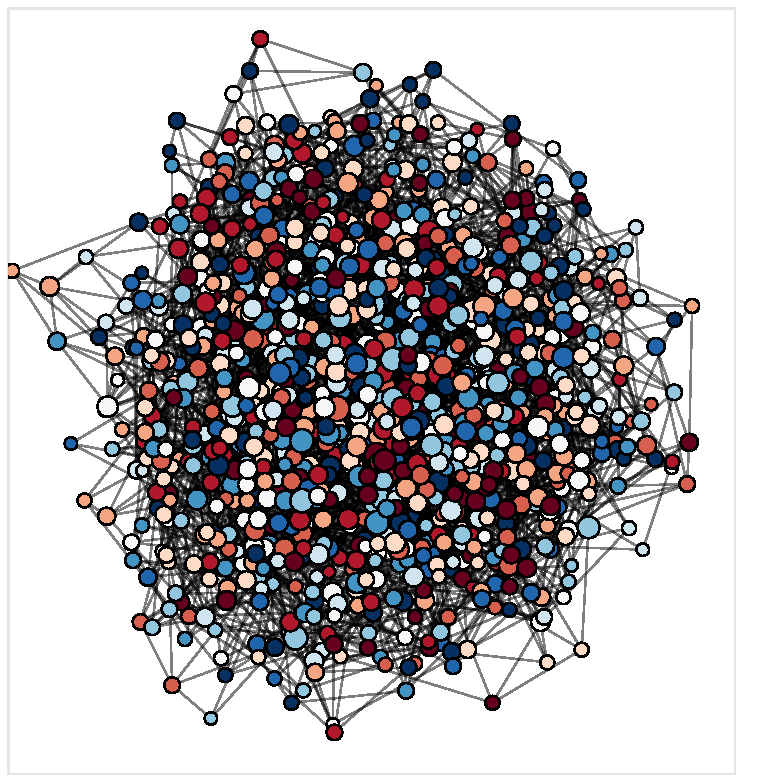
\includegraphics[width=.15\linewidth]{../plots/networks/network_example_R0.3_0.pdf} & 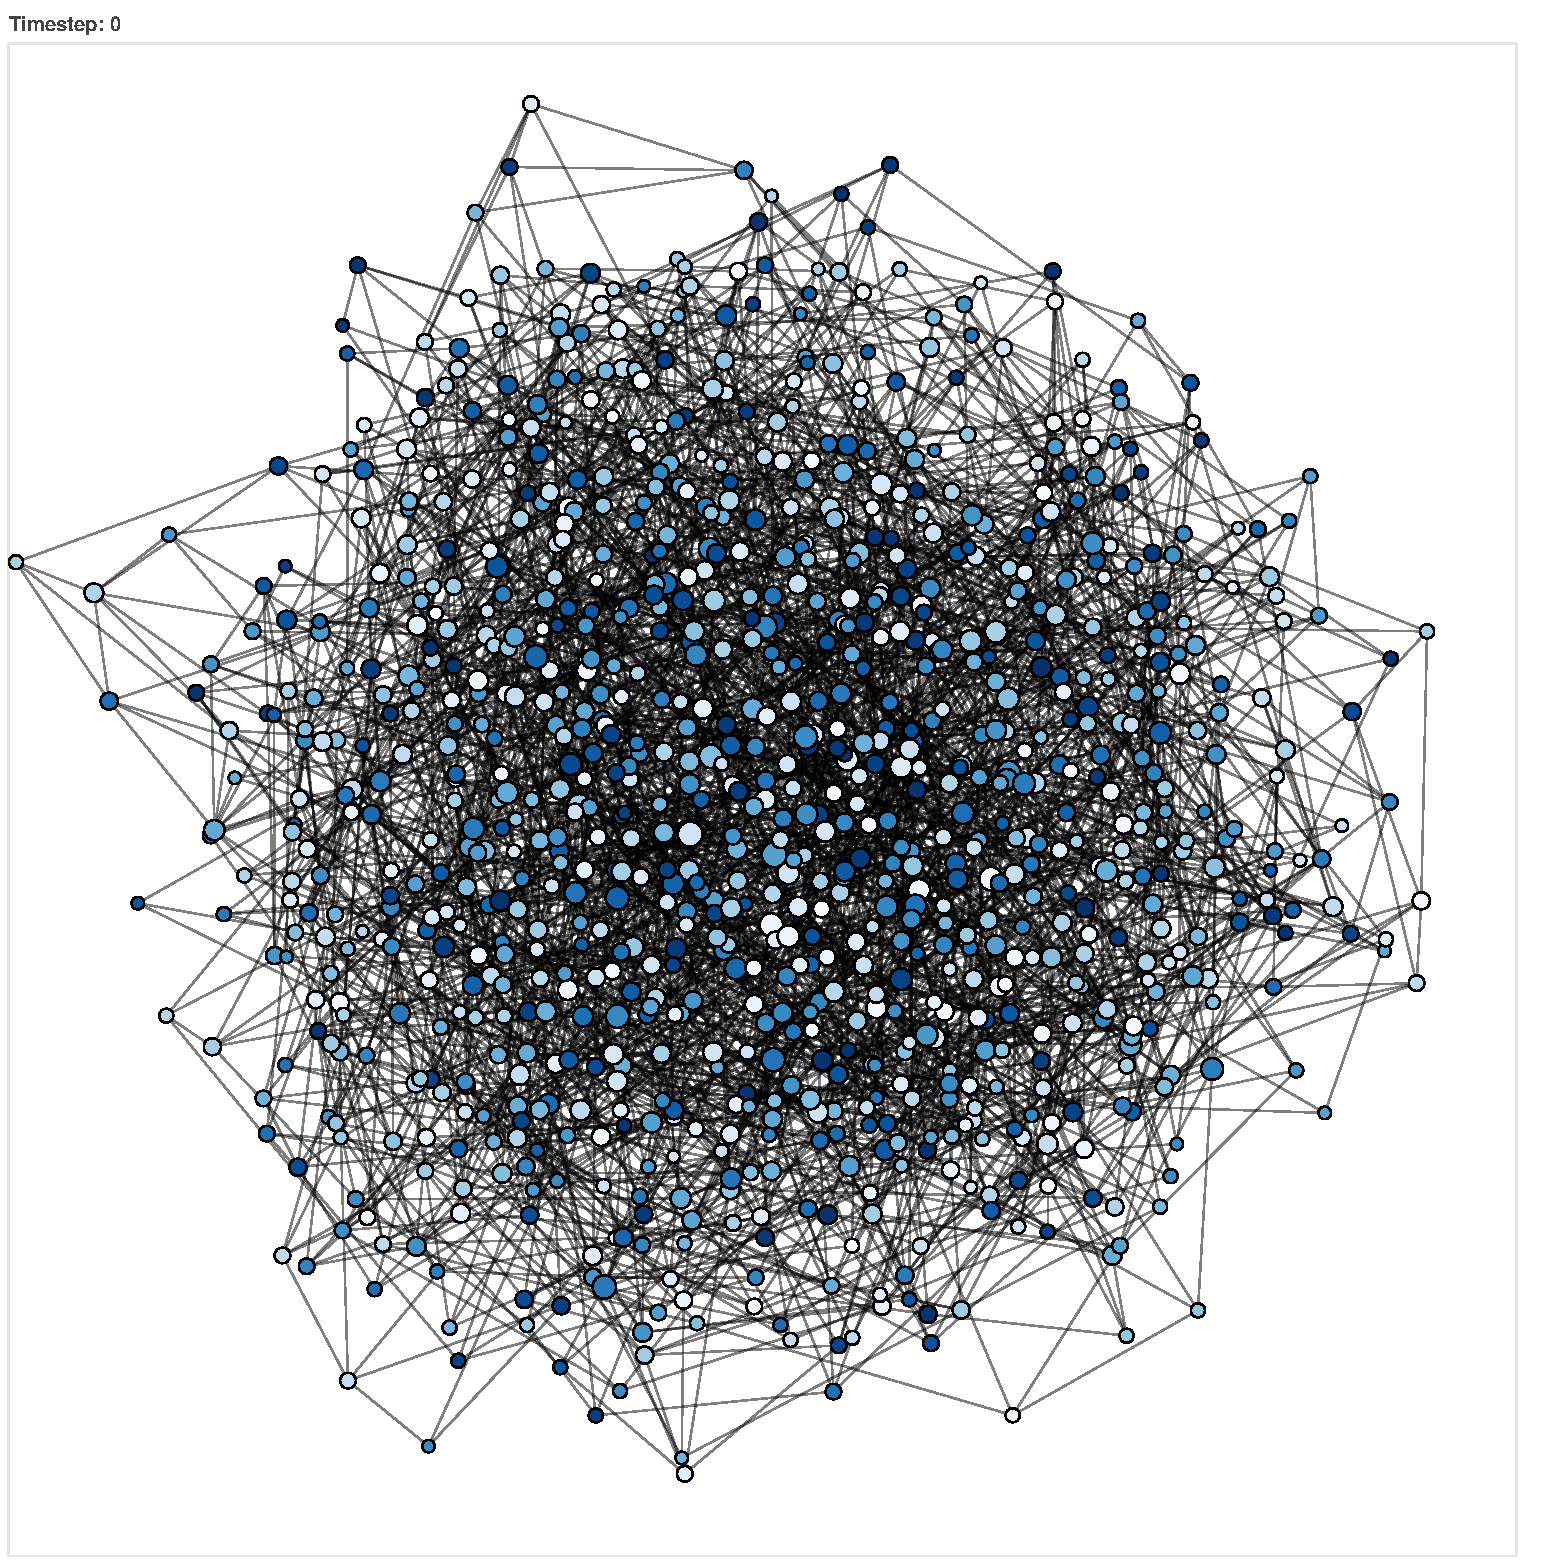
\includegraphics[width=.15\linewidth]{../plots/networks/network_example_R0.5_0.pdf}\\ 
    %\\\hline\\ 
    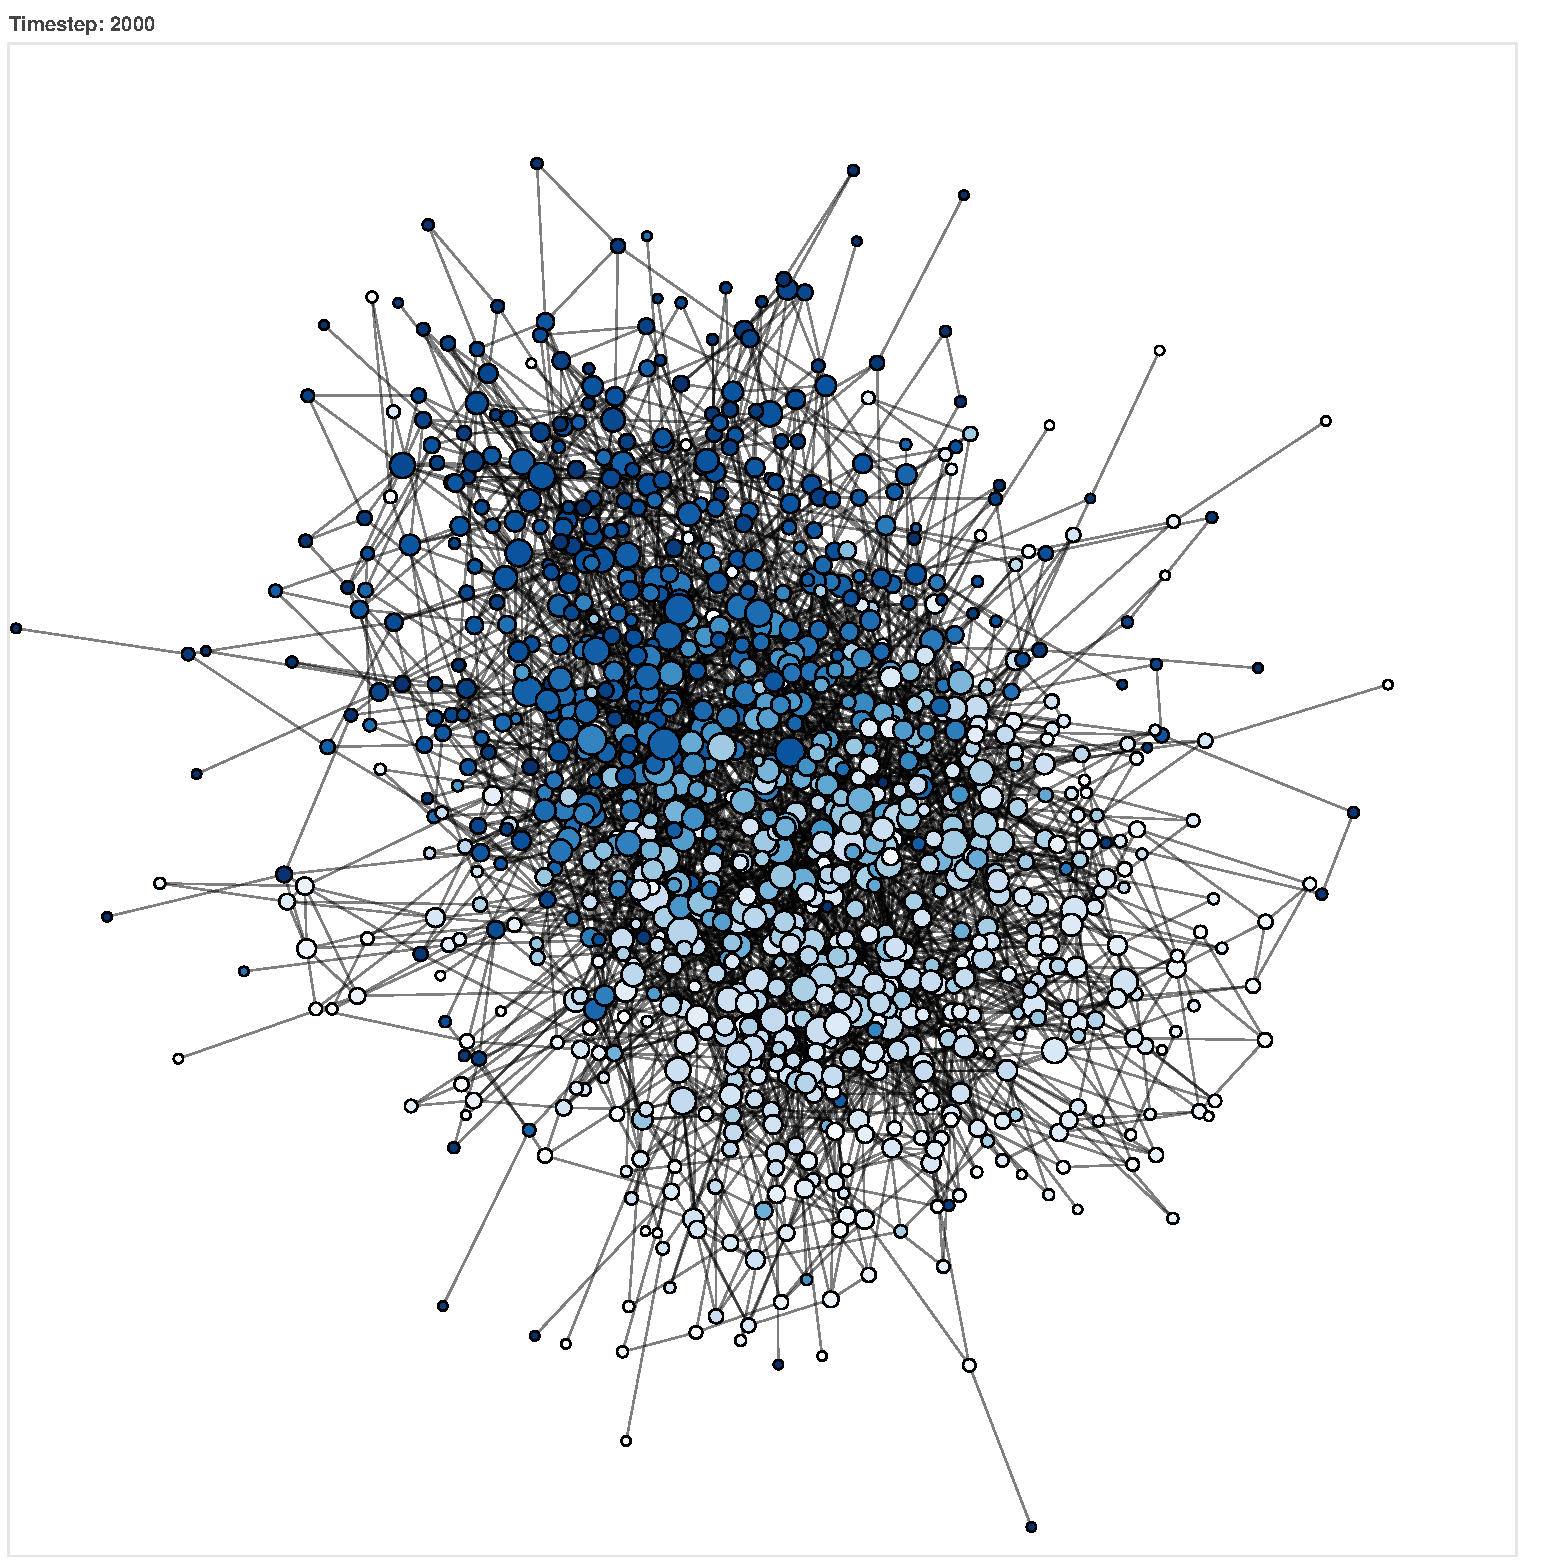
\includegraphics[width=.15\linewidth]{../plots/networks/network_example_R0.1_2000.pdf} & 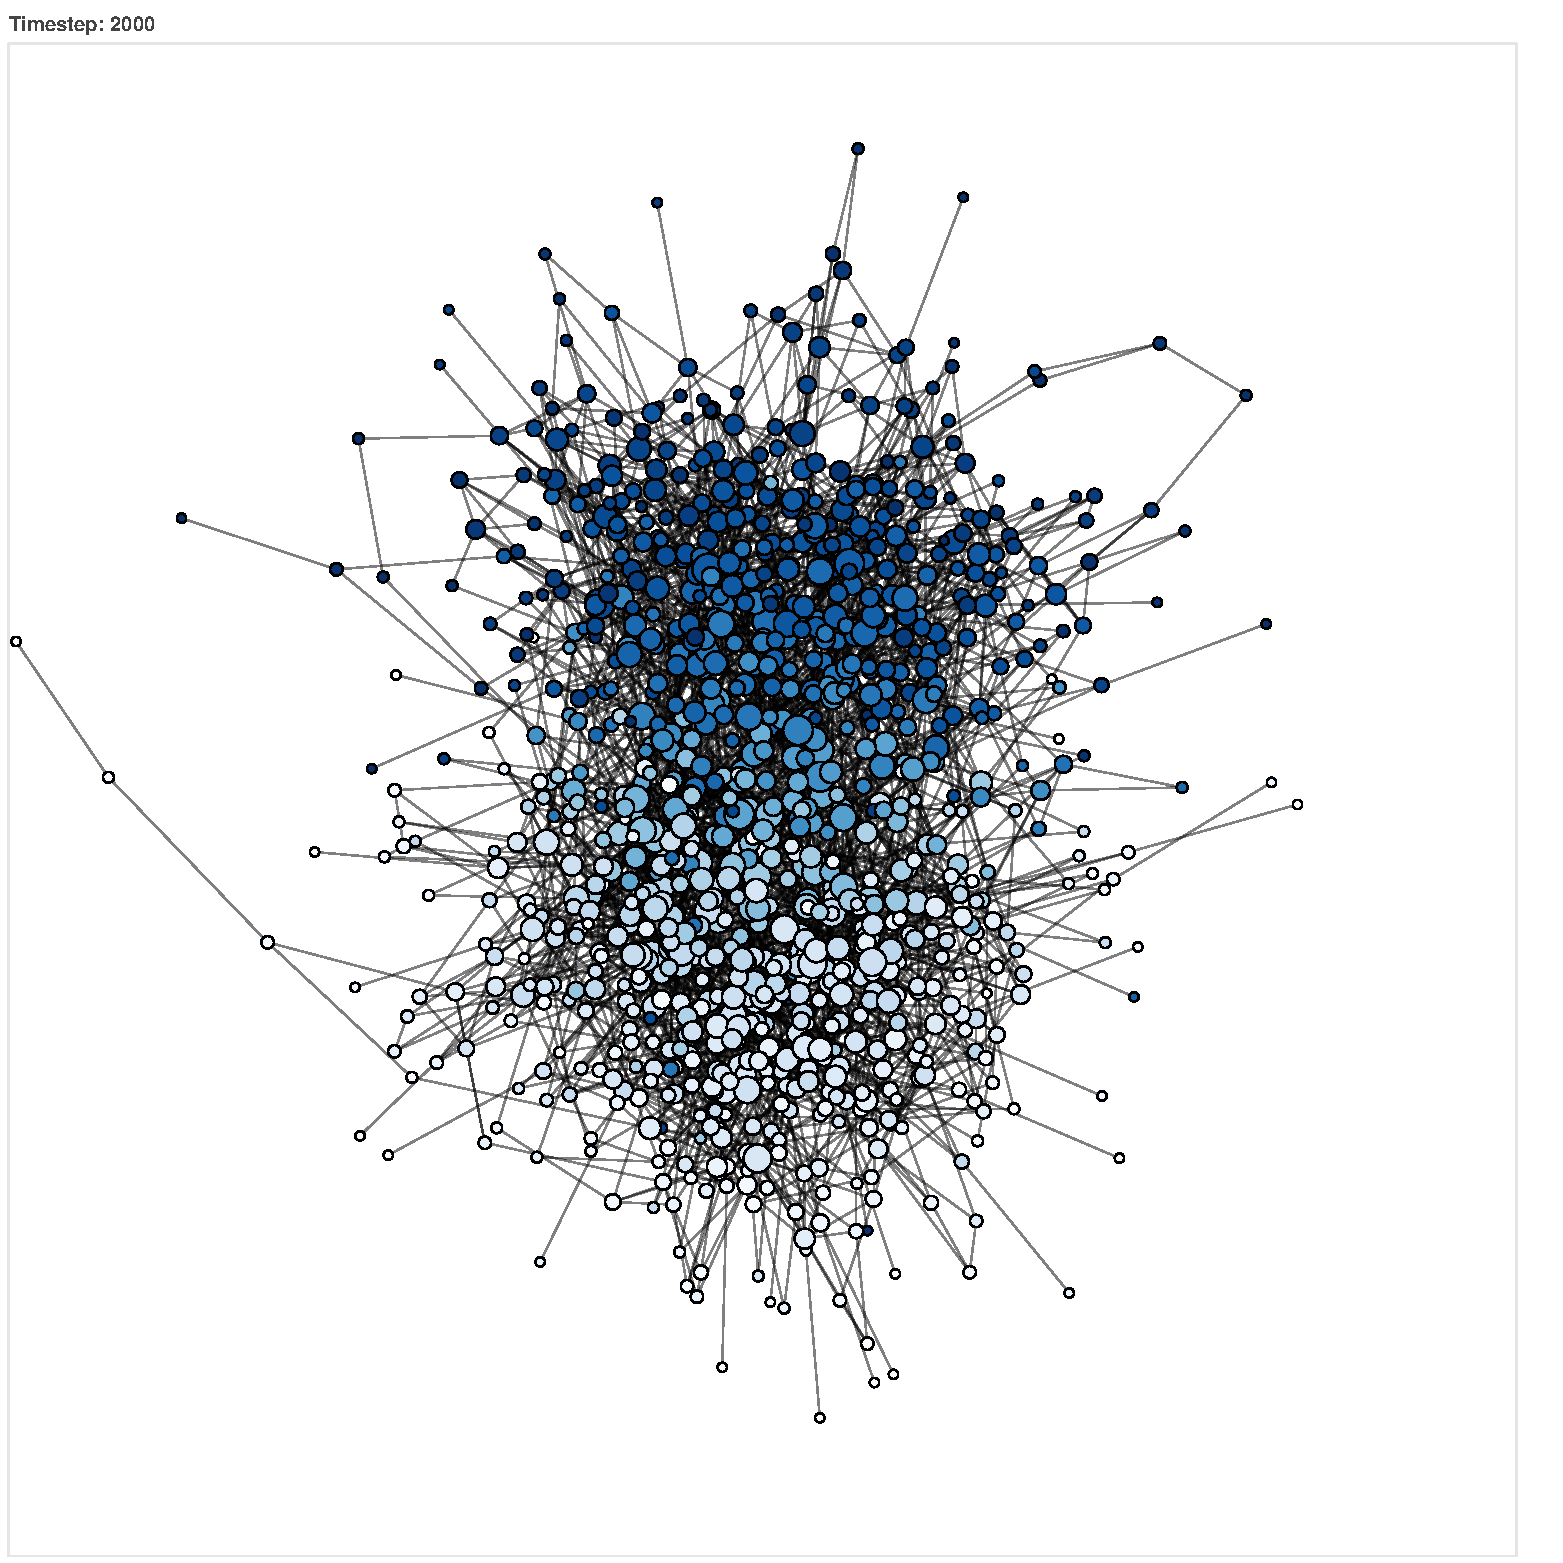
\includegraphics[width=.15\linewidth]{../plots/networks/network_example_R0.3_2000.pdf} & 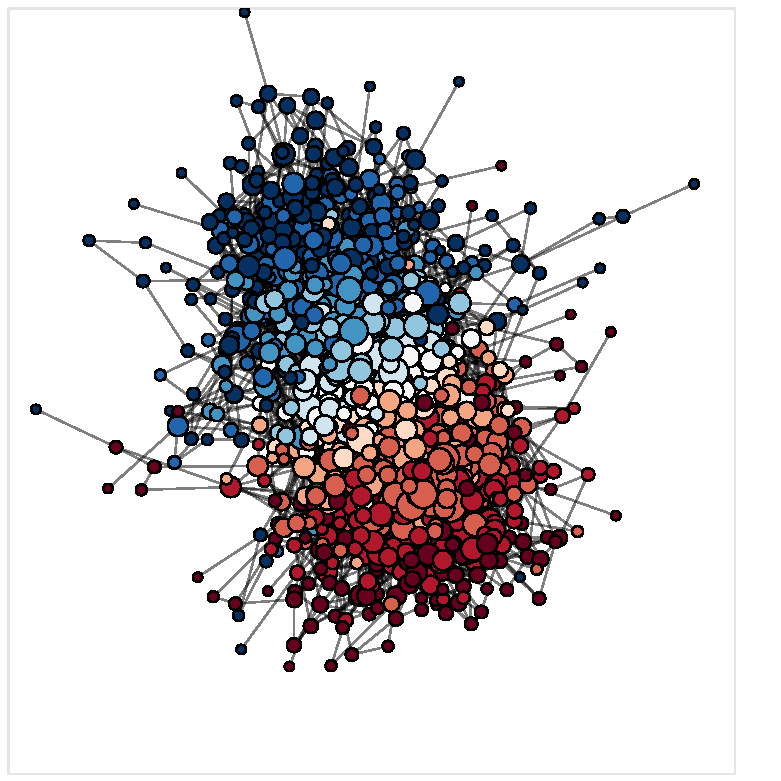
\includegraphics[width=.15\linewidth]{../plots/networks/network_example_R0.5_2000.pdf}\\ 
    %\\\hline\\ 
    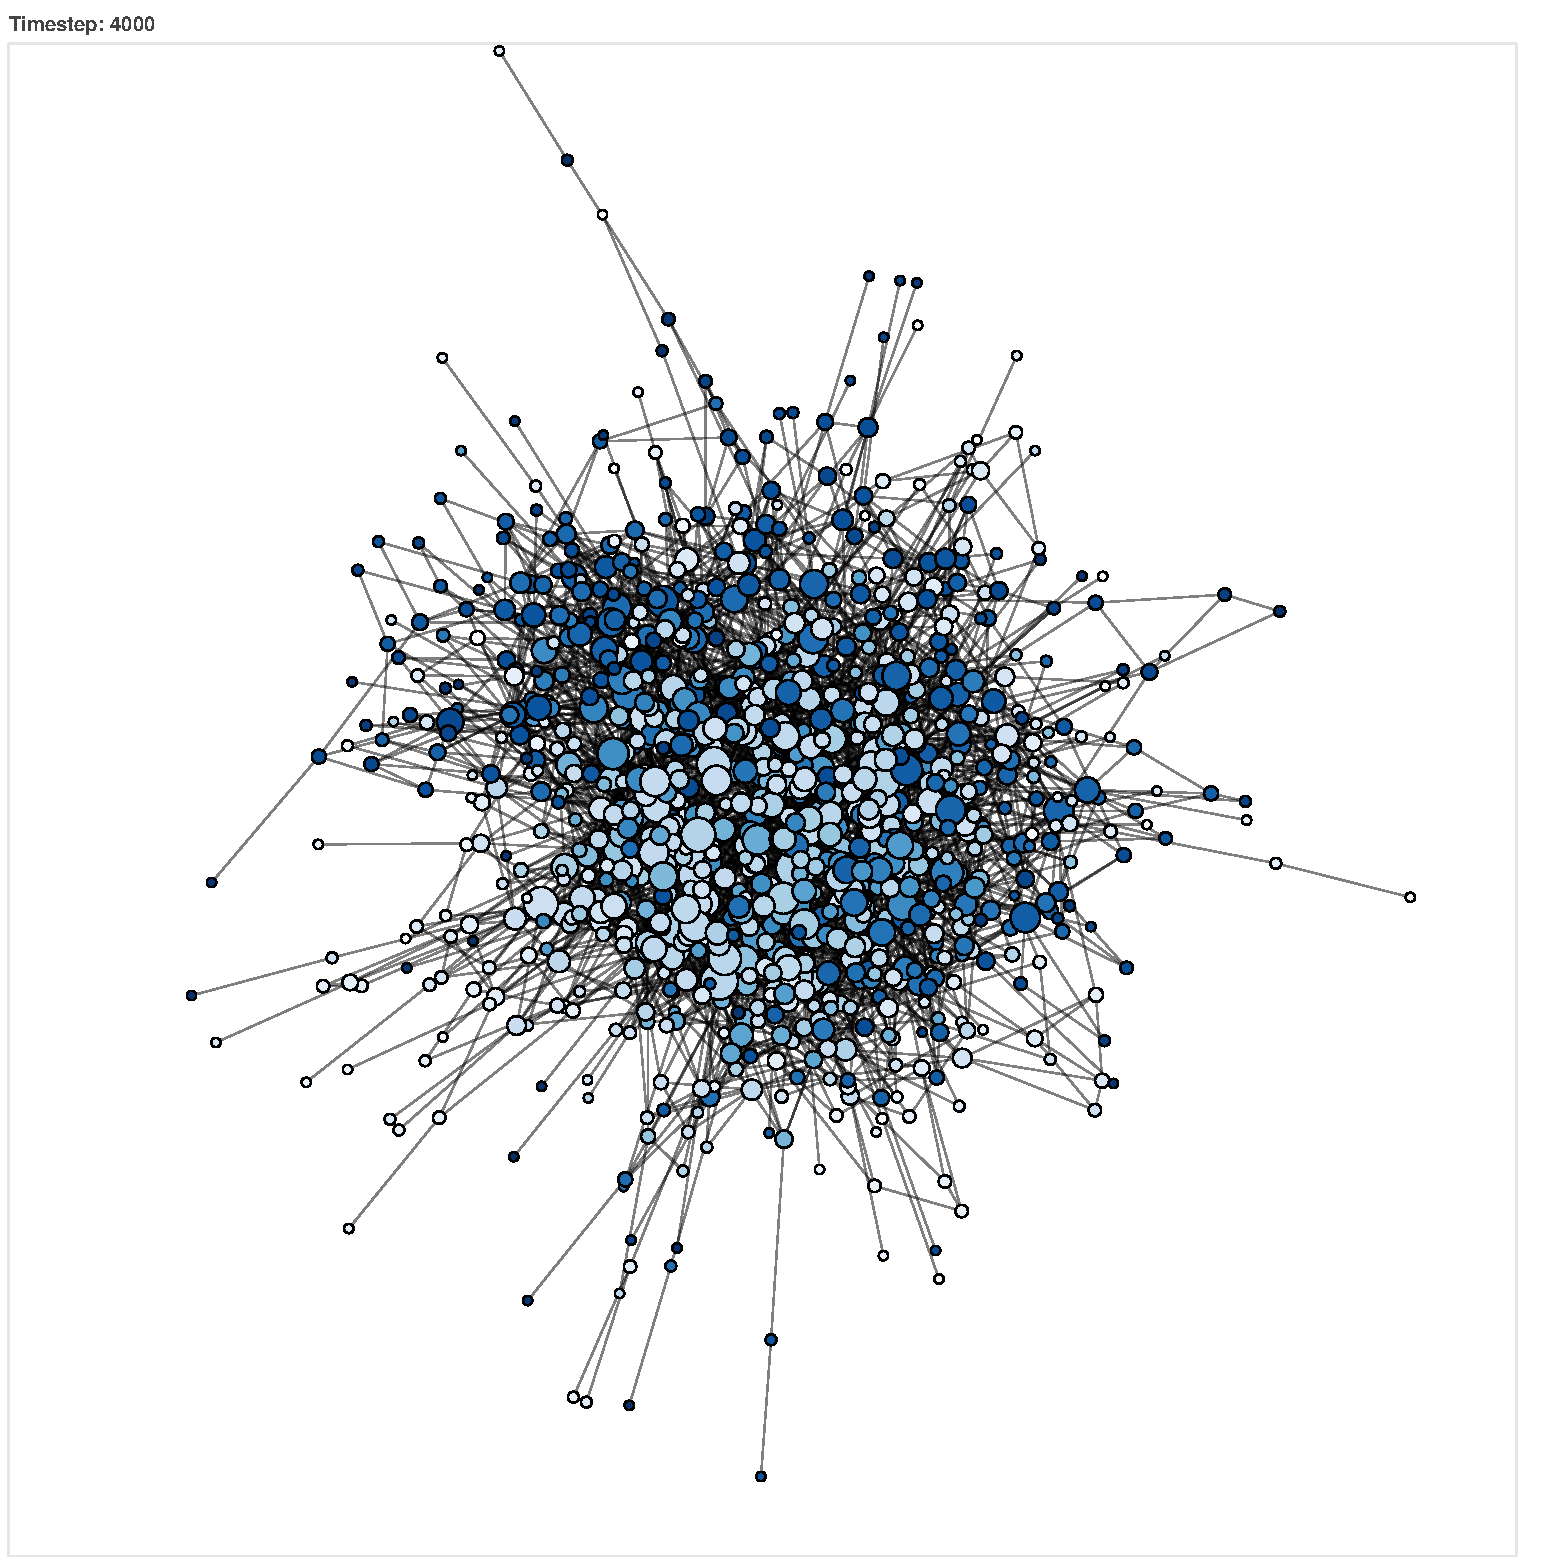
\includegraphics[width=.15\linewidth]{../plots/networks/network_example_R0.1_4000.pdf} & 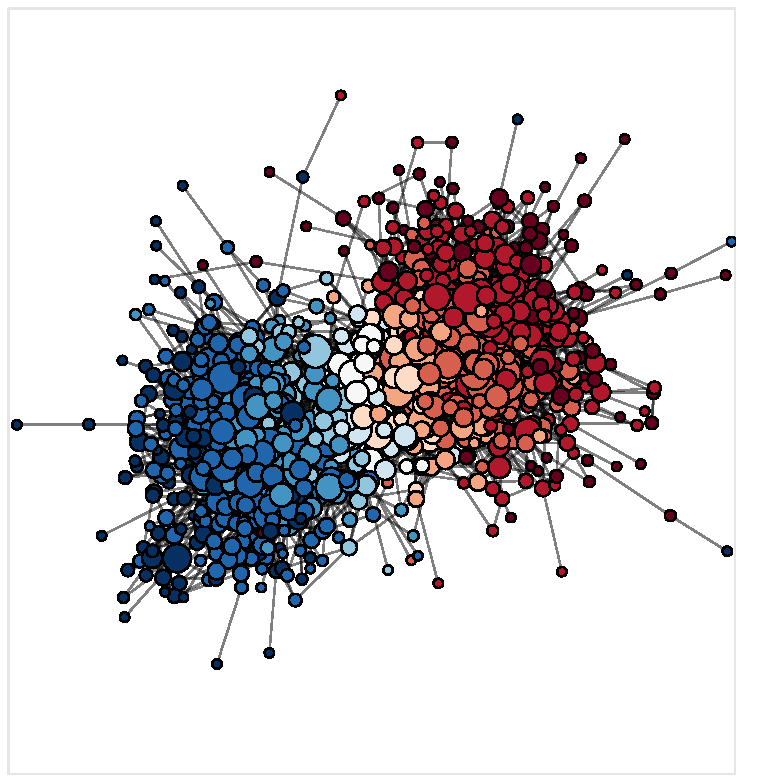
\includegraphics[width=.15\linewidth]{../plots/networks/network_example_R0.3_4000.pdf} & 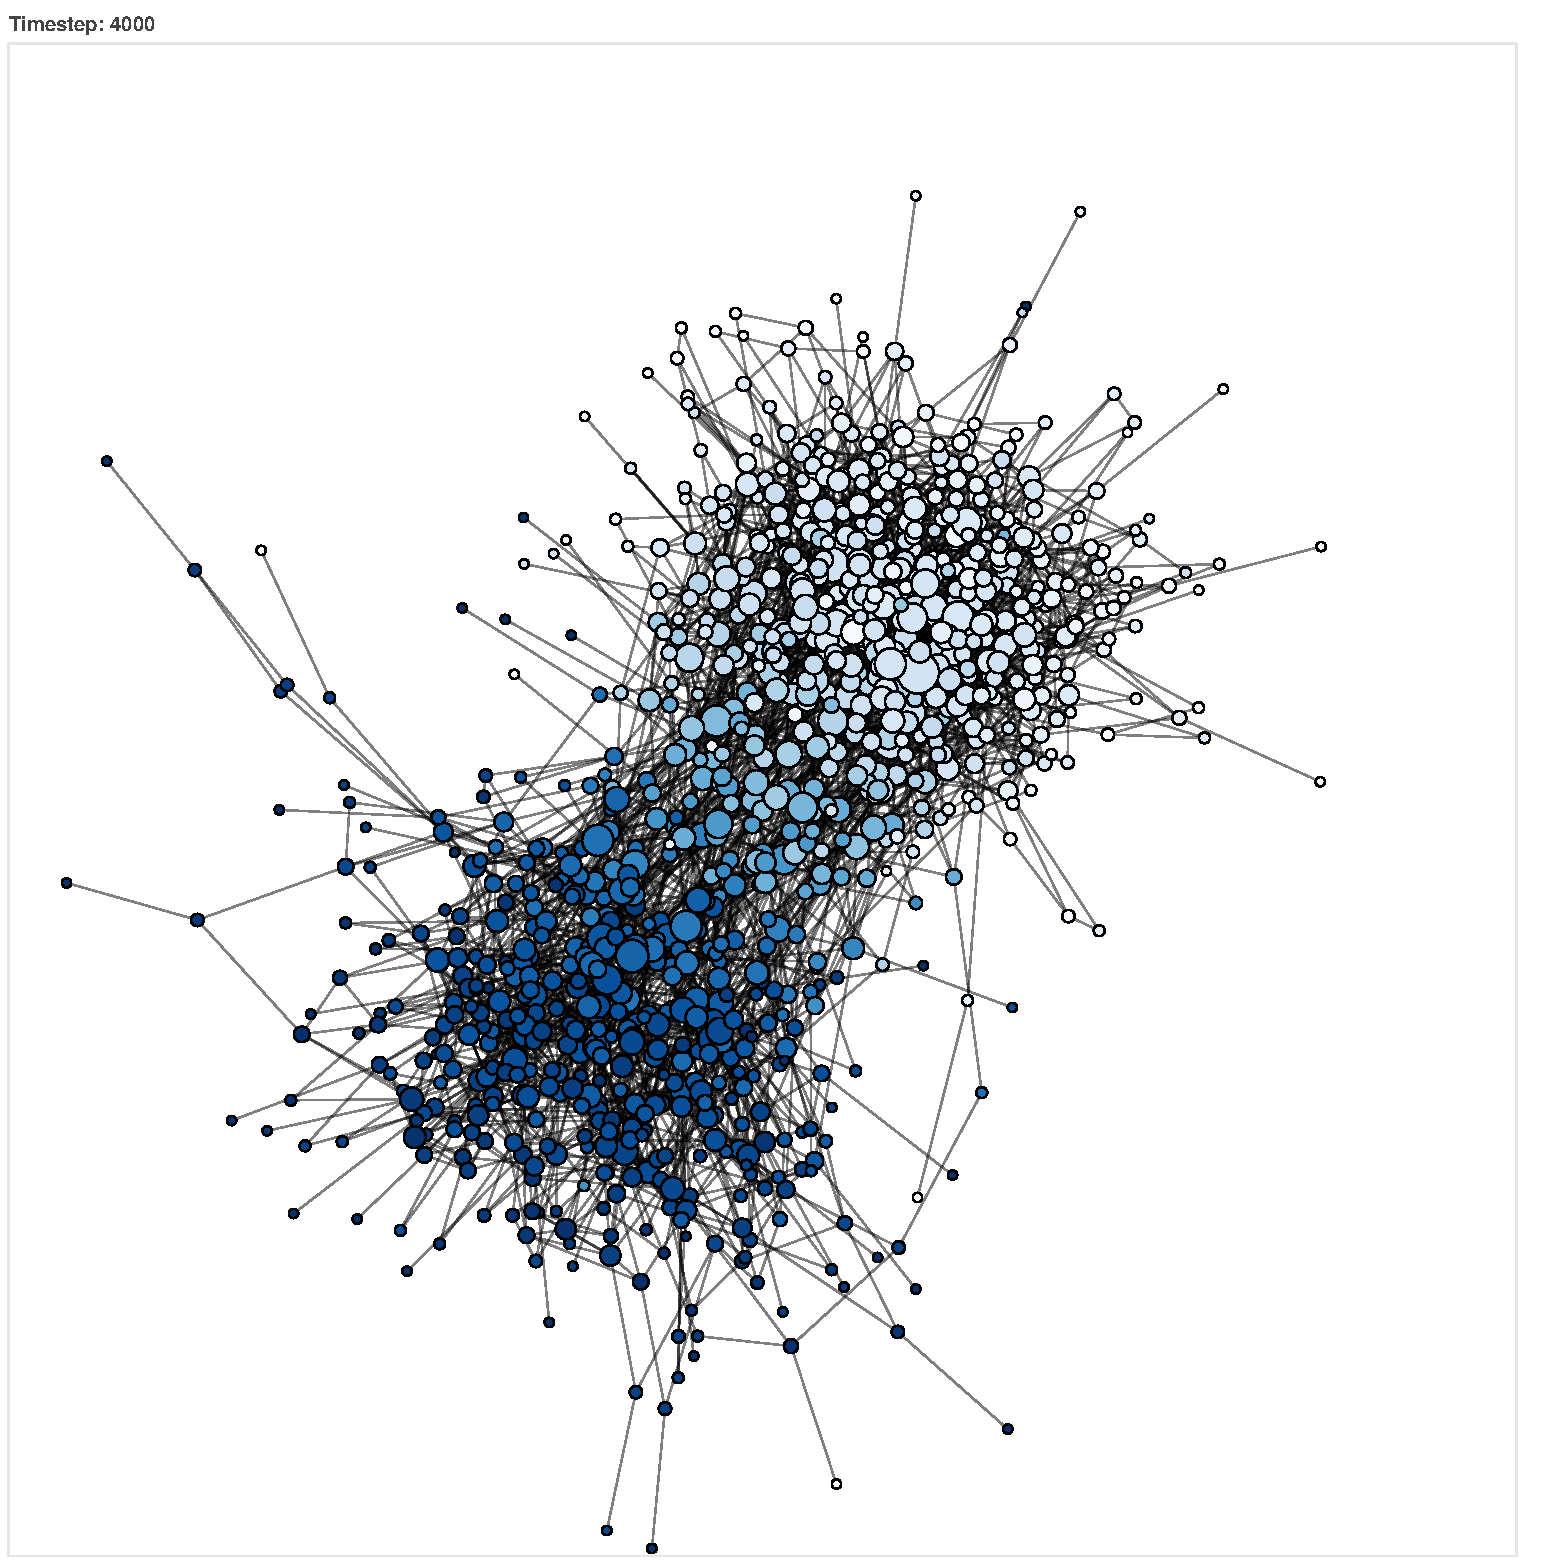
\includegraphics[width=.15\linewidth]{../plots/networks/network_example_R0.5_4000.pdf}\\ 
    %\\\hline\\ 
    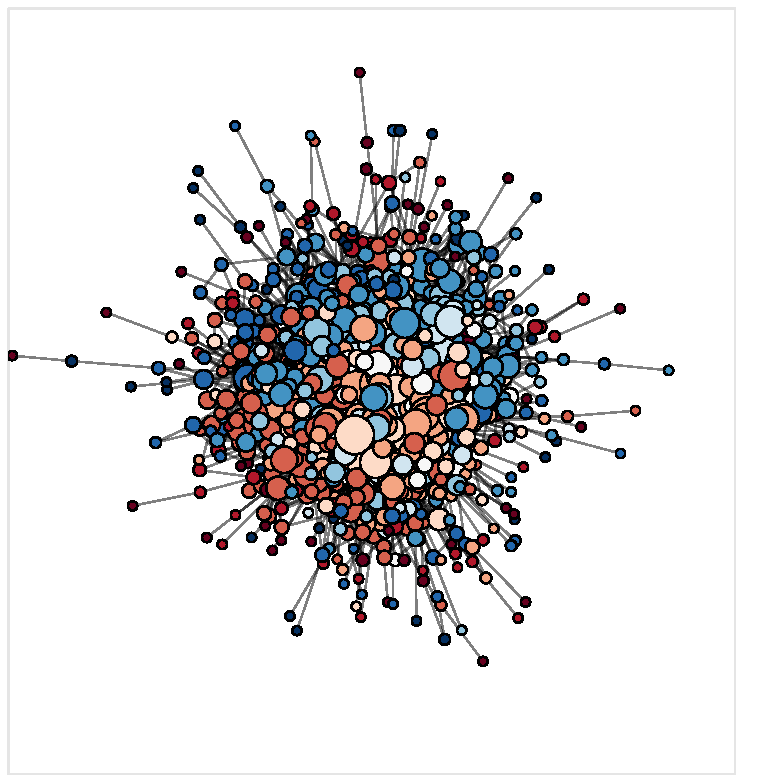
\includegraphics[width=.15\linewidth]{../plots/networks/network_example_R0.1_6000.pdf} & 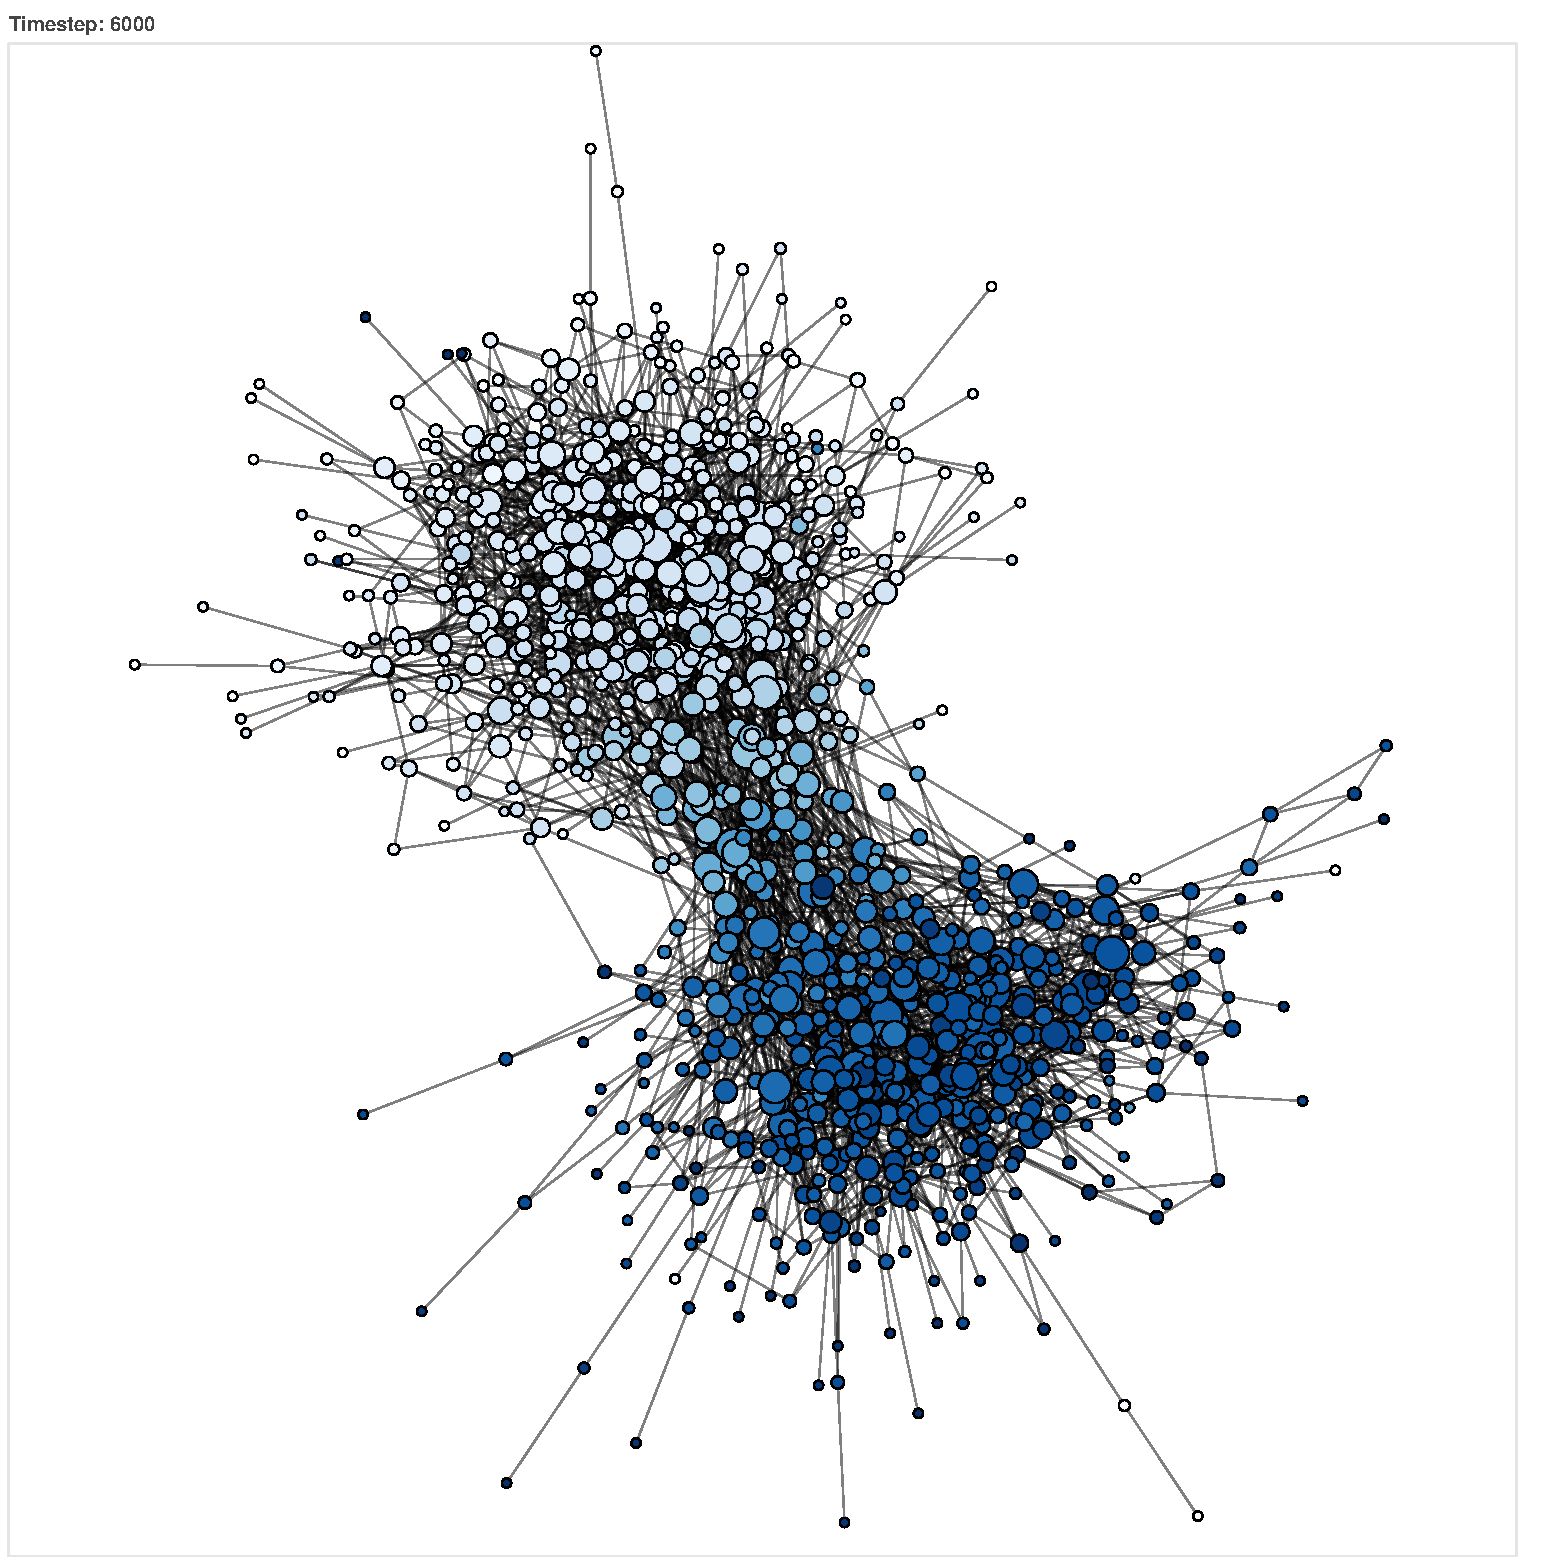
\includegraphics[width=.15\linewidth]{../plots/networks/network_example_R0.3_6000.pdf} & 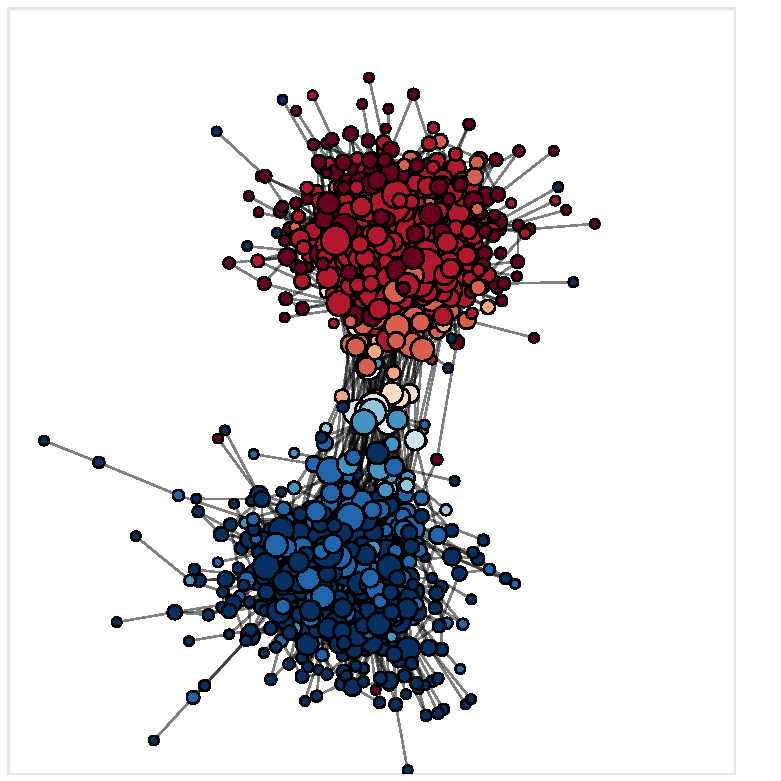
\includegraphics[width=.15\linewidth]{../plots/networks/network_example_R0.5_6000.pdf}\\  
    %\\\hline\\ 
    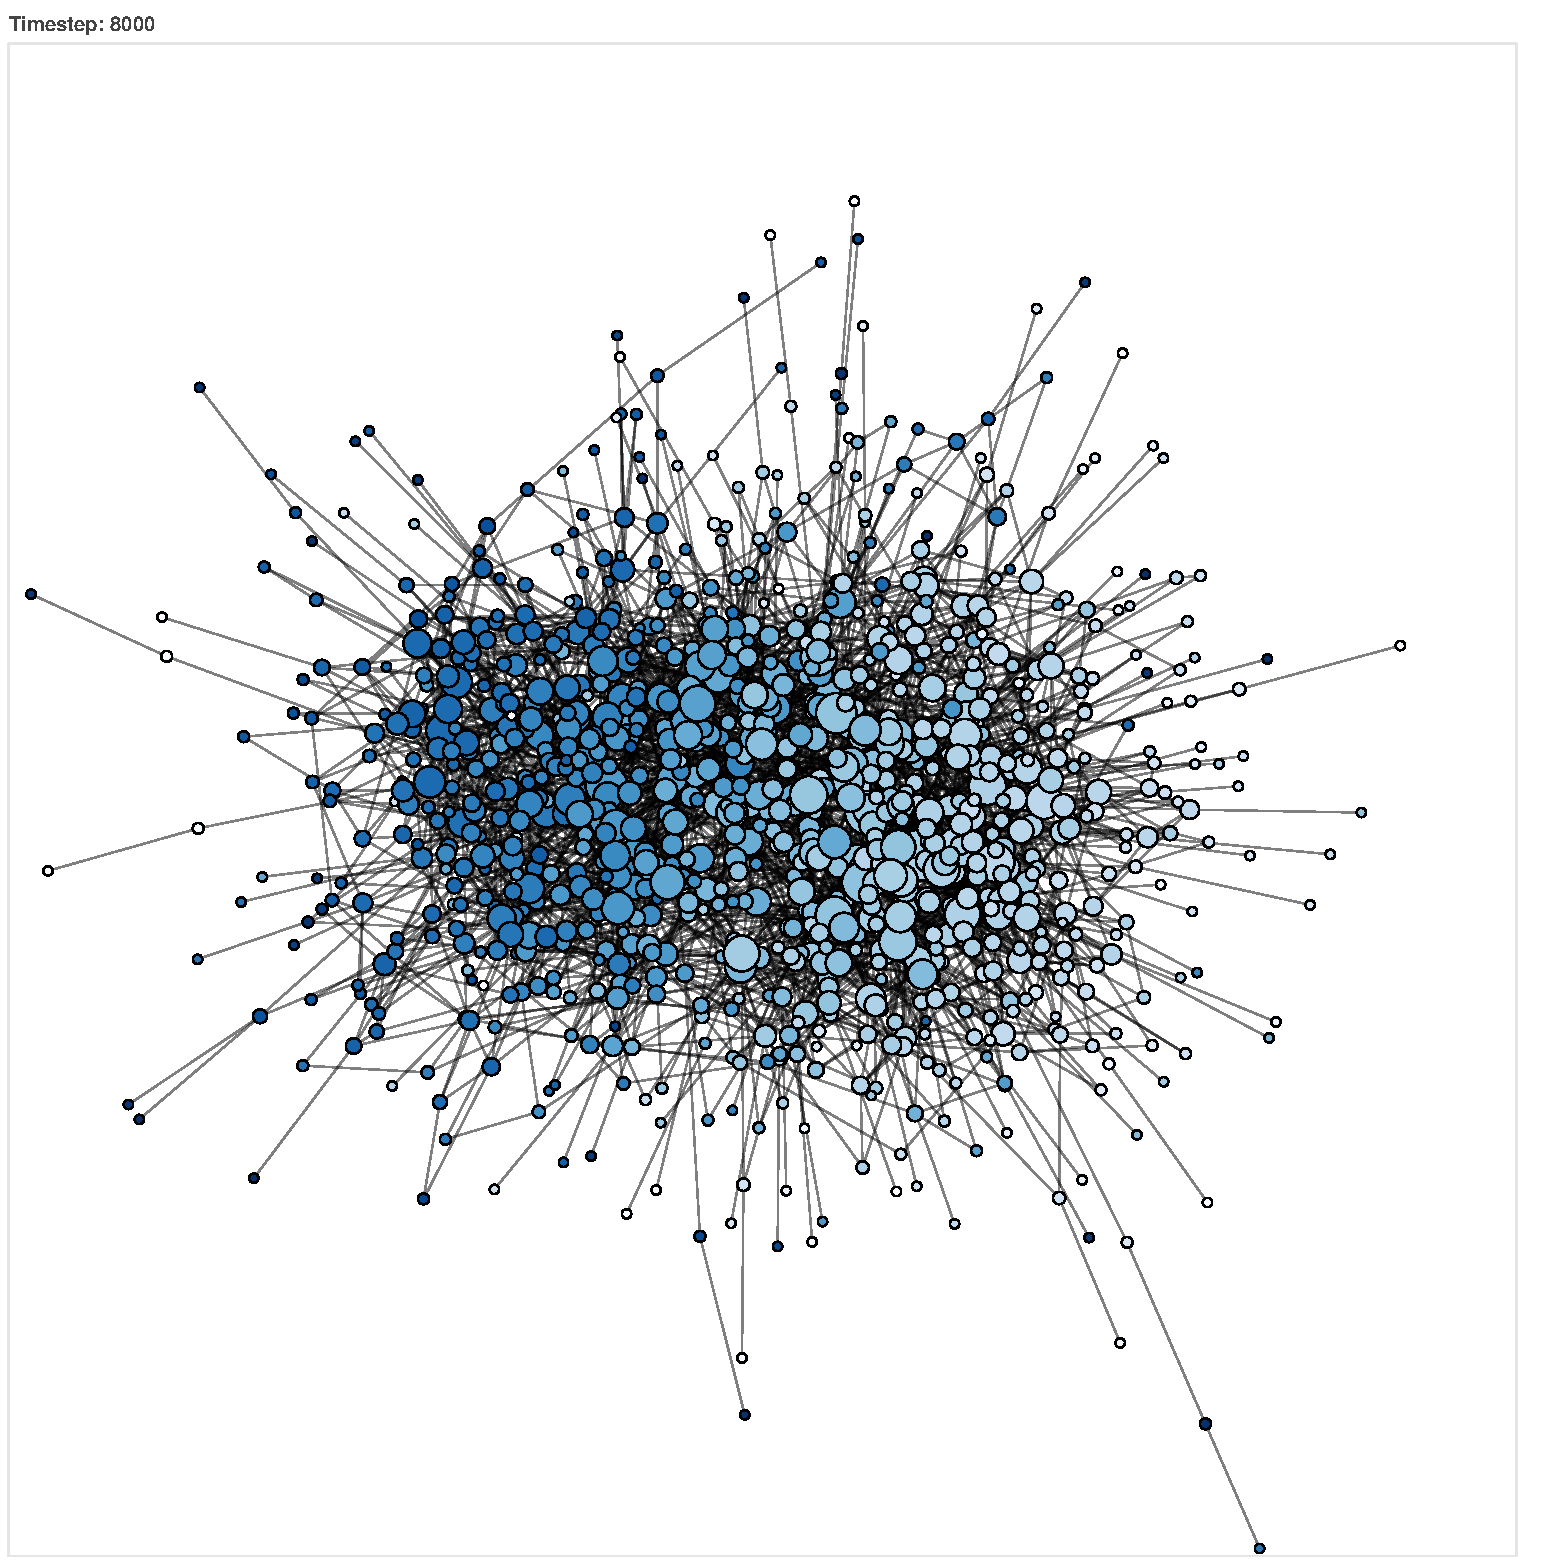
\includegraphics[width=.15\linewidth]{../plots/networks/network_example_R0.1_8000.pdf} & 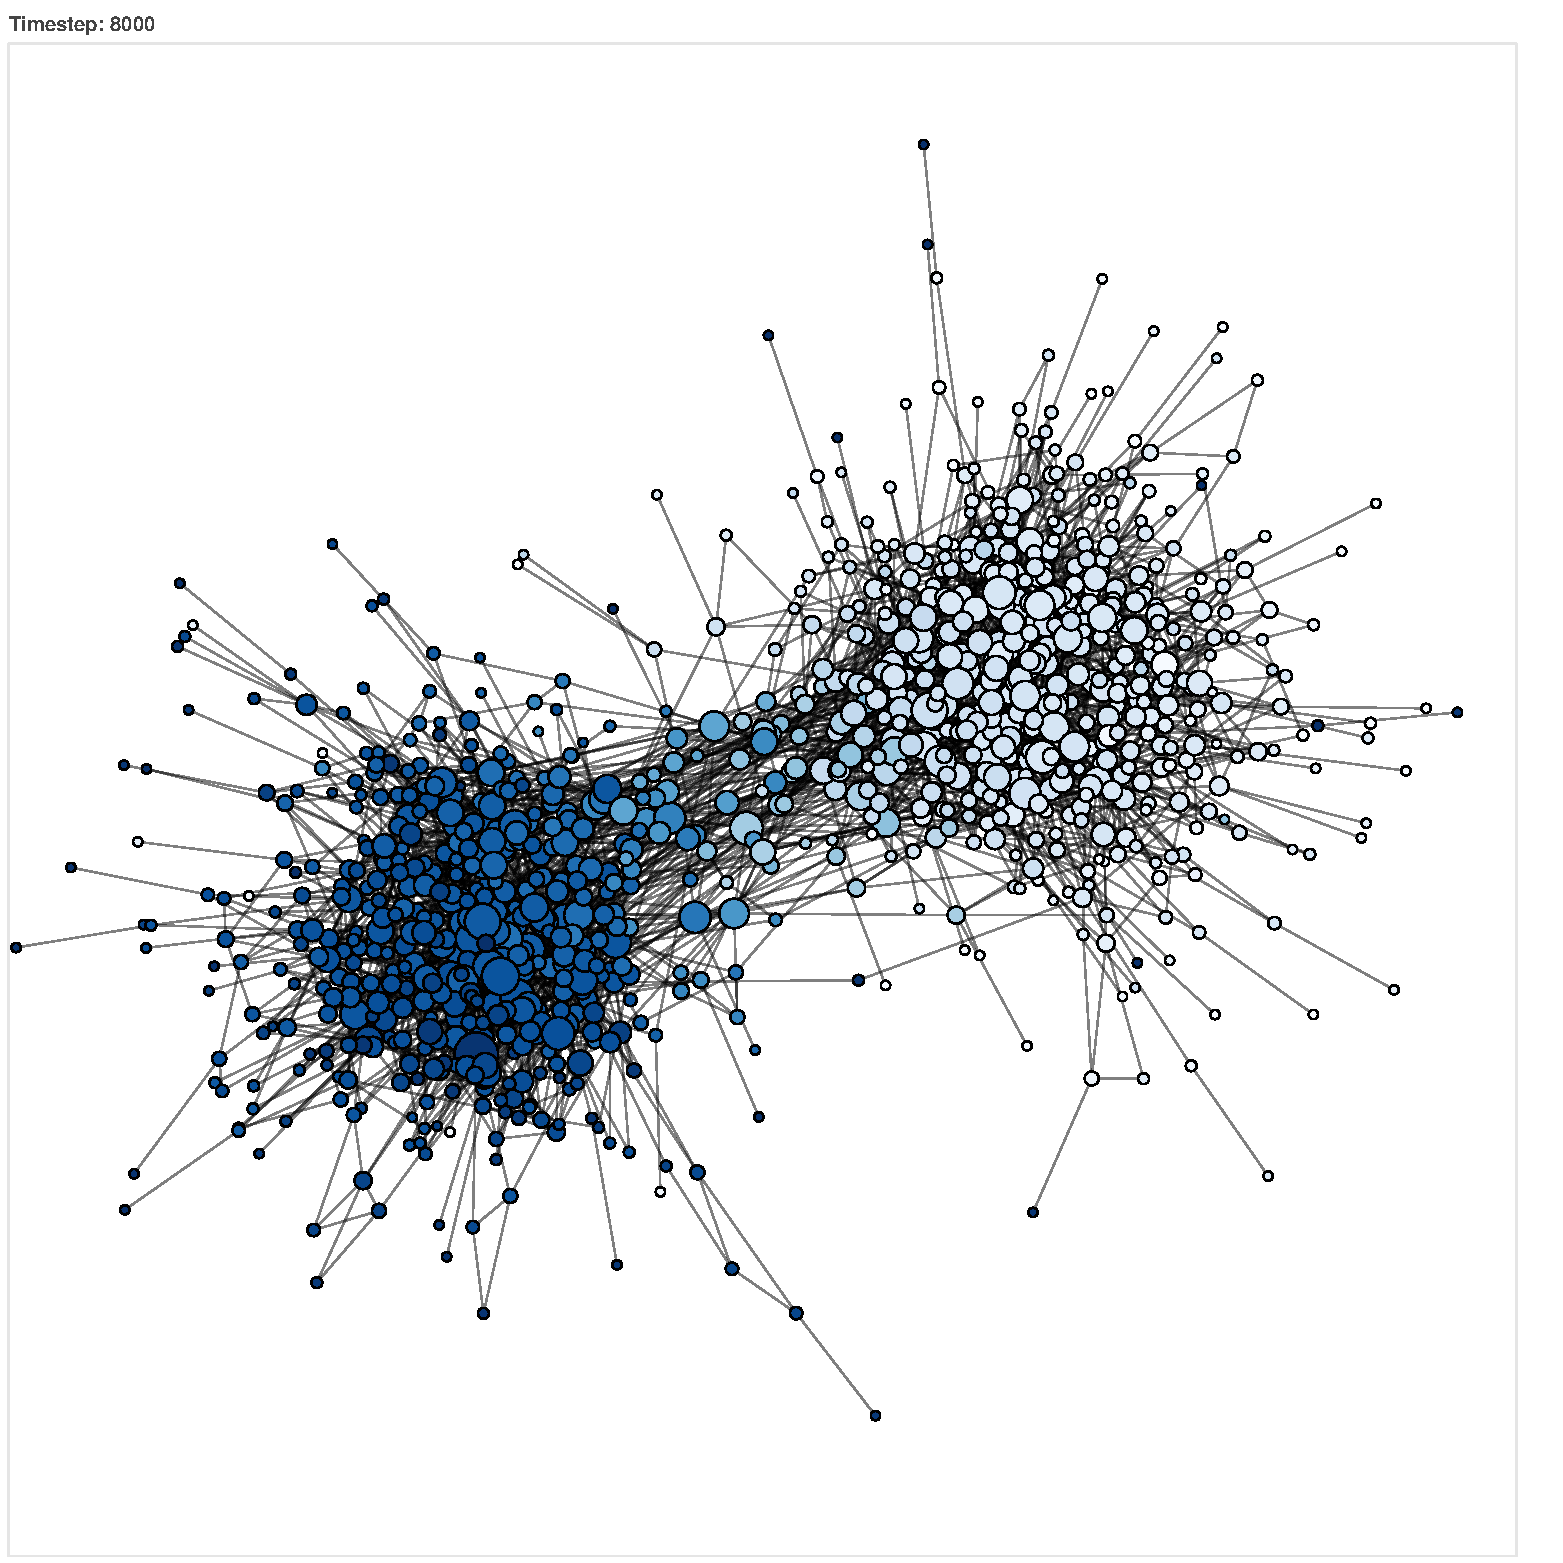
\includegraphics[width=.15\linewidth]{../plots/networks/network_example_R0.3_8000.pdf} & 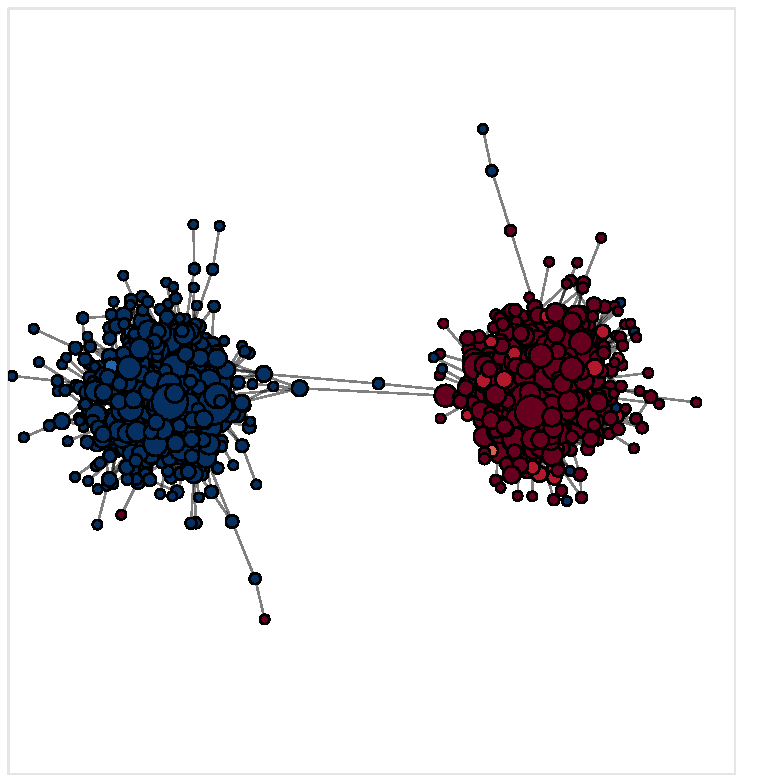
\includegraphics[width=.15\linewidth]{../plots/networks/network_example_R0.5_8000.pdf}\\  
    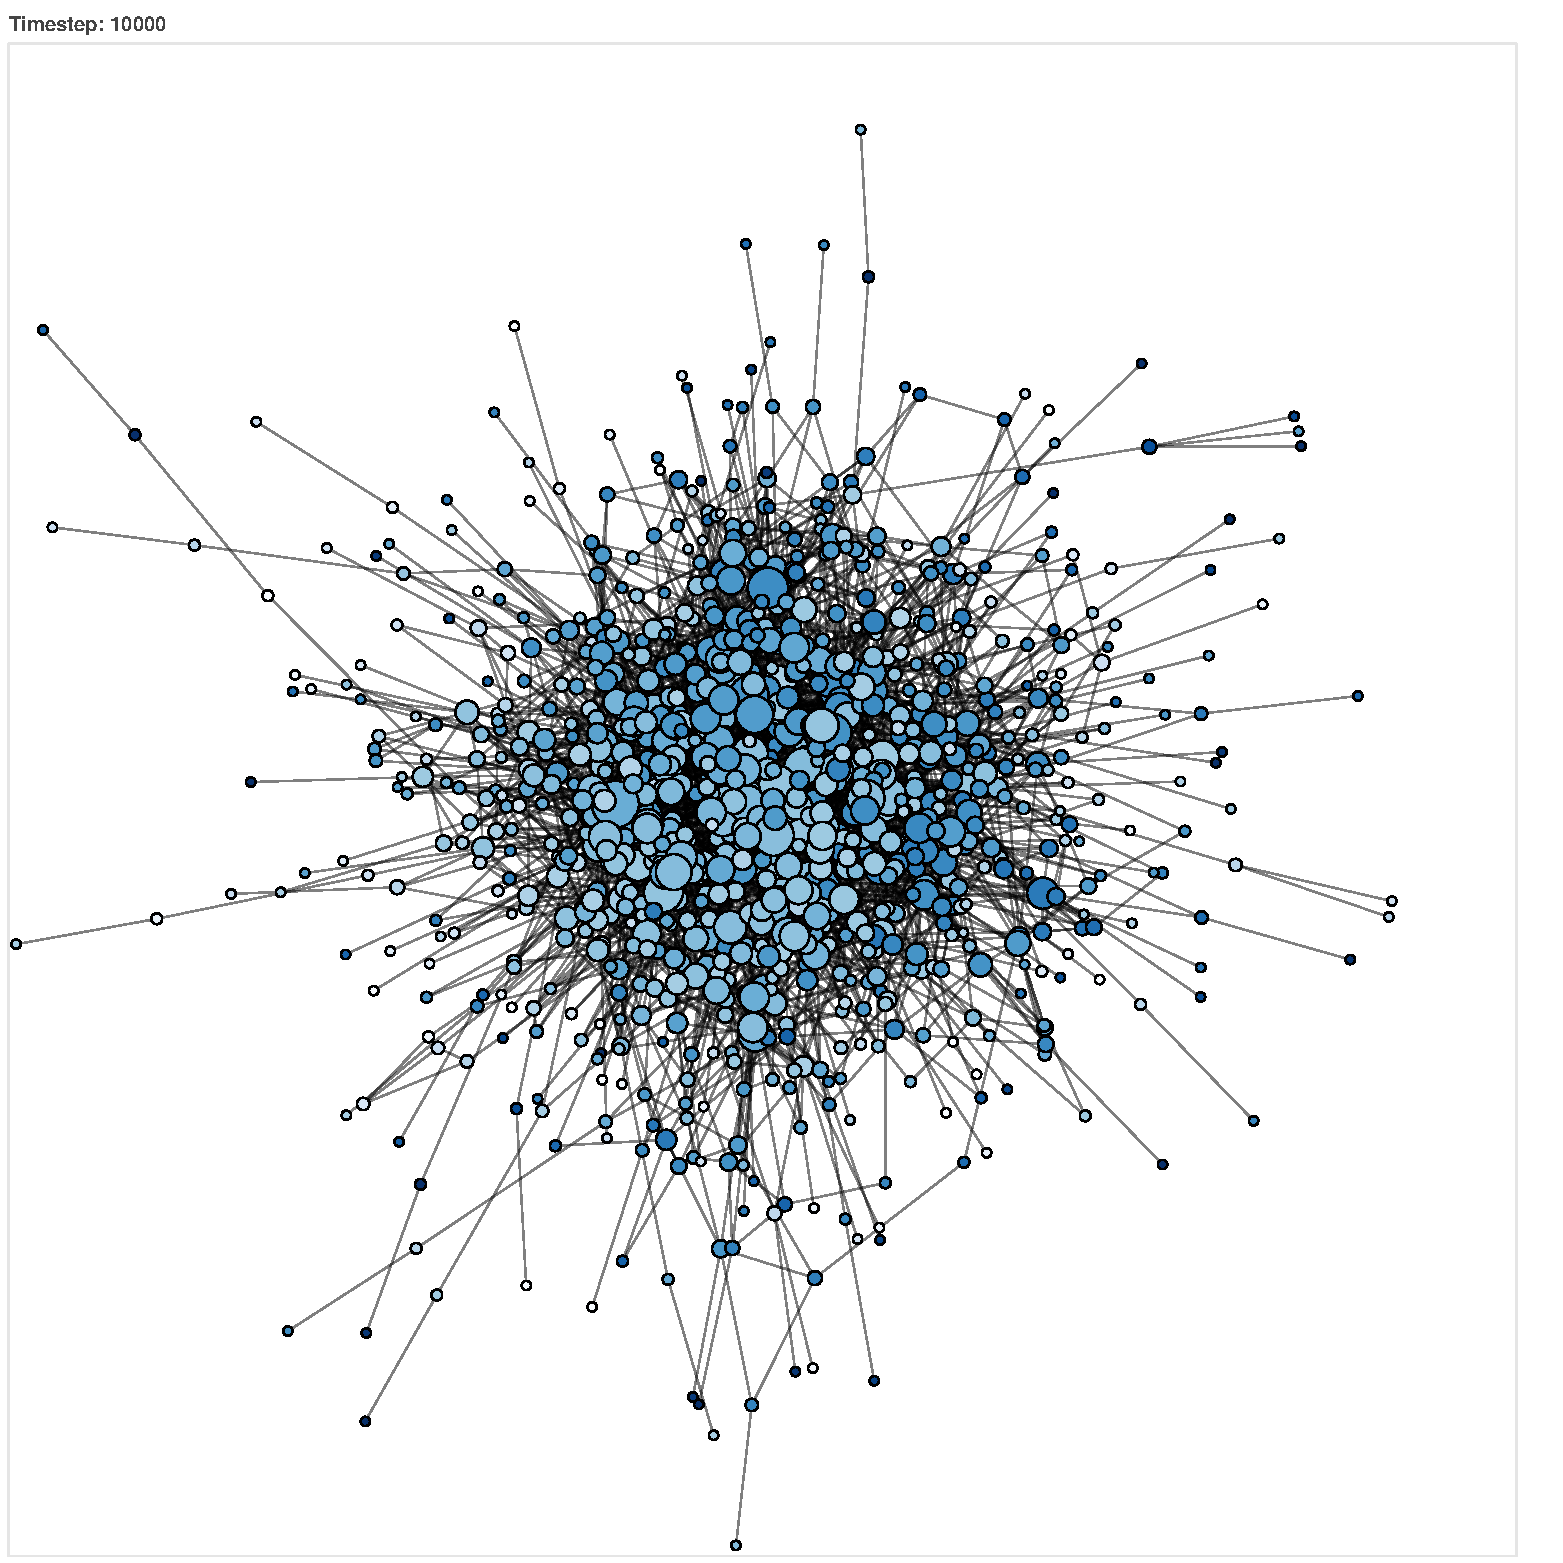
\includegraphics[width=.15\linewidth]{../plots/networks/network_example_R0.1_10000.pdf} & 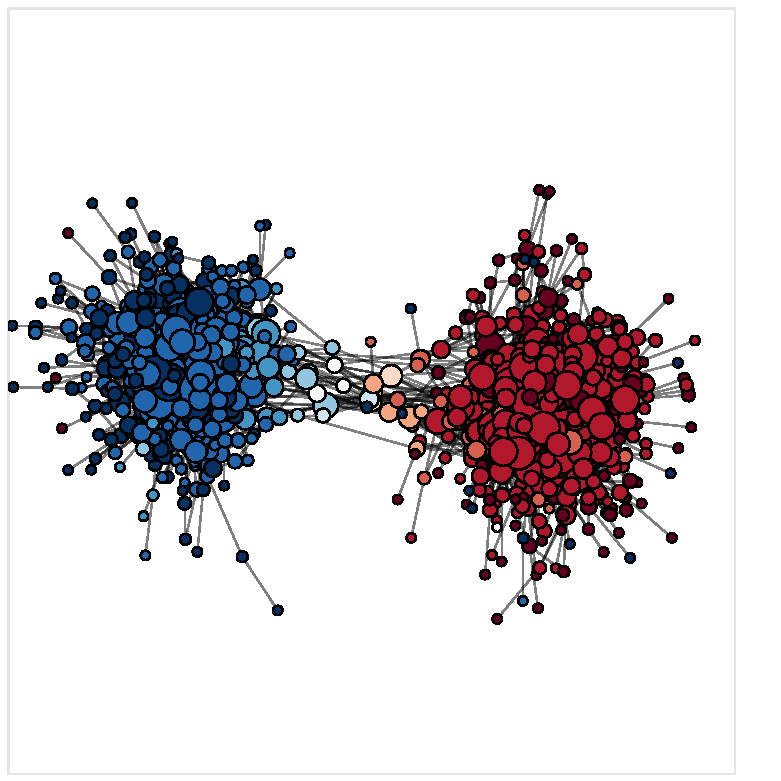
\includegraphics[width=.15\linewidth]{../plots/networks/network_example_R0.3_10000.pdf} & 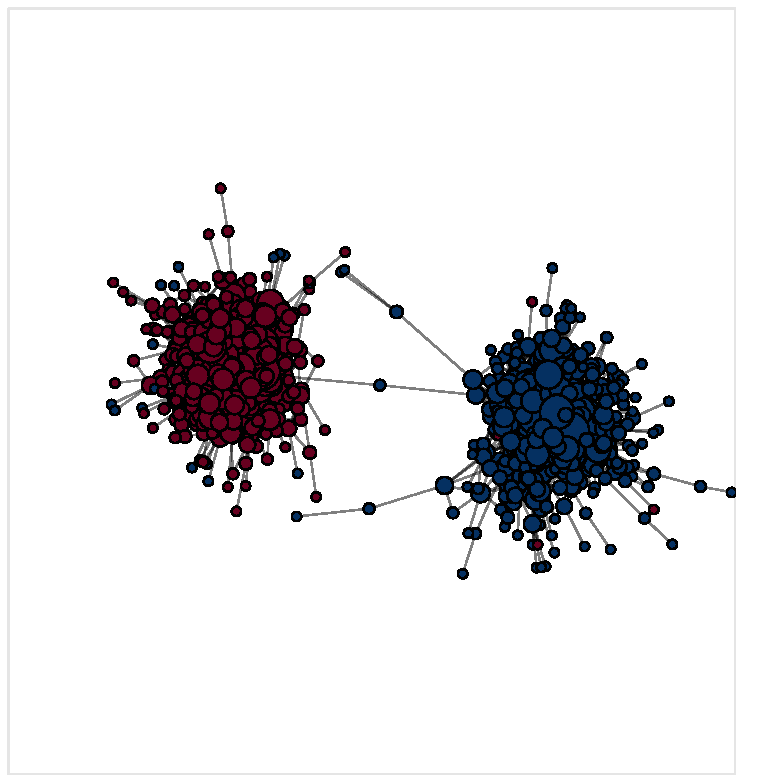
\includegraphics[width=.15\linewidth]{../plots/networks/network_example_R0.5_10000.pdf}\\  
    \end{tabular} 
    \caption{Network evolution for different levels of randomness. Columns show different values of randomness, $R$. Rows are different time-steps of the simulations, increasing in increments of 2000. Nodes represent agents, lines represent edges between agents. Agents are colored by their opinion. Dark blue colors represent values close to -1, and lighter colors represent opinions close to 1. The size of the nodes of agents reflects their degree, with higher degrees shown as larger nodes.} 
    \label{fig:networks} 
    \end{figure} 
\end{center} 
\subsubsection{Distance in opinion and network space}
\noindent The representative simulations also clearly show how polarization in opinions leads to a less globally connected network, which increases the average path length. To see why this happens, one can use a spring as an analogy for the network. As long-range ties are deleted, the tension in the spring rises, and the network starts to be better characterized as a network of two factions, connected mostly by a group of agents with opinions close to 0. As distant parts of the network reconnect, the tension of the spring is lowered, and all the nodes of the network become closely linked again. When polarization increases, there will be fewer long-range ties, but there might also be fewer "middlemen" to facilitate cooperation across the aisle. By middlemen, we refer to the agents of with opinions close to 0, which tend to be situated in between the two main clusters of agents. In the visualizations of the networks, these middlemen are the nodes of cyan colors, that are situated between the two major clusters of dark and light colors (see Figure~\ref{fig:networks}). We draw attention to these agents, as they are critical for the cooperation of the network. Without them, the spring snaps. It does so because the agents of the different clusters cannot have positive interactions with each other, as the average opinion of each cluster will tend to be too dissimilar. By interacting only through these middlemen, there is a chance of bridging the gap by isolating the different groups from each other. If these middlemen become part of either cluster before polarization has decreased sufficiently, the only possible outcome is polarization. The existence of middlemen is therefore a necessary condition for avoiding polarization in this model. 

\subsection{The importance of speed}
\noindent Another way to understand why polarization can be prevented by negative tie-deletion, is to realize that the probability of tie-deletion can be interpreted as the rate at which the structure of the network adjusts to opinions. When $P(D) = 1$, the structure of the network adjusts at the same speed as opinions, while lower values indicate that the network adjusts at a slower pace than opinions. In this interpretation, consensus can be achieved if the social network adjusts fast enough. Having faster adjustment of the structure of social interactions is critical because the system is highly path-dependent \cite{turner_paths_2018, macy2021polarization}.  When the network doesn't adjust fast enough, agents will already have had several negative interactions, which will typically have pushed them further towards an extreme value of opinions. This will make them more likely to polarize other agents in the future. This will be the case for all agents including the middlemen, that are necessary for reaching consensus. Adjusting too slowly can therefore burn the only bridge that is available for preventing polarization.  

\subsubsection{The point of no return for polarization}
The simulations investigated in detail here also highlight the fact that there seem to be points of no return regarding polarization. This is primarily because polarization breeds more polarization. If the system as a whole reaches a critical tipping point of polarization, the system will not be able to reach consensus as polarization becomes self-reinforcing (see Appendix~\ref{appendix:ponr}). The same conclusion is found in recent models of polarization where exogenous shocks to the system, such as a global pandemic, create a common threat for all agents \cite{macy2021polarization, levin_dynamics_2021}. They find that if a system has already reached a certain level of polarization, even powerful exogenous shocks are not enough to make agents cooperate with each other. They find that if a system is already heavily polarized, it is almost impossible to introduce measures that can depolarize the system. Although identifying such tipping points is not the focus of this paper, the results still show that early countermeasures are essential to avoid polarization (see Appendix~\ref{appendix:ponr}).

\part{Overall Discussion}
Our central finding is that co-evolution of opinion and network dynamics is a vital factor to consider in explaining both systems. This conclusion is based on both the empirical data integration as well as the study of the Co-evolutionary model. The empirical data integration shows that models which include opinion dynamics can drastically outperform network formation models when the target networks are large and opinionated. The results from the Co-evolutionary model show, that co-evolution is vital for explaining how social systems can avoid polarization in the face of mechanisms such as negative social influence. Without co-evolution, even small amounts of negative social influence can cause the system to polarize (see Figure~\ref{fig:radicalization}). 
In both cases, the reason why co-evolution becomes so vital is that co-evolution allows for a systematic mechanism for generating multiple communities in the network. Not only is this the phenomenon that makes the Co-evolutionary model a better explanation for large, opinionated networks than network formation models, but it is also the phenomenon that explains how tie-deletion can prevent polarization. By generating two distinct communities, social exposure to the opposing group is minimized, which limits the effect of negative social influence (see Figure~\ref{fig:networks}).

\noindent The analysis also highlights that many of the emergent properties of social networks can be generated by surprisingly simple mechanisms. The model considered here does not include mechanisms of choice homophily nor does it include agents with a goal or a strategy. By including only negative tie-deletion as a co-evolutionary mechanism, the model can generate realistic social networks better than the most used social network generating models. By including opinion dynamics, the model can also produce emergent properties such as the connection between distance in similarity and distance in the social network as seen in empirical studies \cite{kossinets_origins_2009} (see Figure~\ref{fig:distance_similarity}). However, one should be hesitant to conclude that tie-deletion of dissimilar agents is the most important generating mechanism that gives rise to these properties in social networks. As was alluded to in the case study of representative simulations, tie-deletion is important because it increases positive assortment. Previous results show that similar results could be achieved by implementing a mechanism of choice homophily instead, where agents connect to other agents based on how similar they are \cite{asikainen_cumulative_2020}. A model based on choice homophily instead of negative tie-deletion would only produce similar results to the ones found here if these new connections were rewired primarily from dissimilar agents. If this is not the case, it is unlikely that the model would be able to avoid the negative social influence which comes about from having opinions be randomly distributed. 

If social agents choose new social ties based on how similar they are, i.e. choice homophily, one must assume that these agents can process information about the other agent before interacting with them. This is not an unrealistic assumption, as the choice of clothes and other social markers provide effective ways of identity signaling \cite{smaldino_models_2022}. Here we show that observed homophily can occur even when agents do not share information, but purely through structural homophily. Structural homophily in the model emerges because of the important interaction between tie-deletion and triadic closure. This also highlights how important triadic closure is as a generating mechanism for social systems. As we saw in the second part of this paper, triadic closure alone can generate many of the characteristics associated with social networks. This is in line with results from previous implementations of similar mechanisms in other models \cite{jacksonsearch2004, jacksonmeeting2007}. When triadic closure is combined with homophily and social influence, the interaction between these mechanisms can explain more complicated social phenomena such as community formation. Previous work suggests that the interaction of triadic closure with homophily can also generate core-periphery structures in social networks, which is another staple feature of social networks \cite{asikainen_cumulative_2020}. The same interaction also has a substantial impact on how opinions change over time in computational simulations (see Figure~\ref{fig:pd}, ~\ref{fig:networks}). This is an important note as previous work focusing on dynamical networks in opinion dynamics does not include empirically motivated network dynamics, but simply generates new ties at random \cite{kozma2008consensus}. Here we show that the inclusion of even simple, realistic network dynamics can have large effects on opinion dynamics (see Figure~\ref{fig:pd}). 

\section{Contrast to previous work}
The agent-based model presented here is similar in many ways to the model presented in the \textit{\nameref{introduction}}, which investigate the emergence of echo chambers in social networks \cite{sasahara_social_2021}. Despite their similarity, they find opposite results regarding negative tie-deletion. Contrary to our findings, \citeA{sasahara_social_2021} report that increasing negative tie-deletion accelerates polarization. It is therefore important to understand why these results are in so stark contrast. First, the network considered in \citeA{sasahara_social_2021} is a directed network, meaning that relations need not be reciprocal. This could have important implications because it allows for social influence to be asymmetric. Second, the number of agents considered in \citeA{sasahara_social_2021} is only 100 whereas it is 1000 in the model presented here. This could also be consequential. As we've seen in the representative simulations, tie-deletions can only prevent polarization if there are enough middlemen that can reunite the different clusters. Simply having more agents in the simulation increases the number of expected middlemen, which can help in facilitating cooperation between agents of very different opinions. 

Perhaps the most critical difference between the models is that \citeA{sasahara_social_2021} does not include negative social influence in their model. In the model of \citeA{sasahara_social_2021}, social relations outside the threshold of agents have no social influence. In other words, negative interactions are assumed to be without a cost for the agents involved. For the parameter values considered in the model presented here, tie-deletion is only effectively preventing polarization when there is negative social influence in the system (see Figure~\ref{fig:pd_no_negative}). 
As the main difference between these models is whether forces akin to negative social influence push distant opinions apart, more research needs to be done regarding how pervasive forces like negative social influence are. Such forces do not have to be negative social influence specifically. Whenever the costs outweigh the benefits associated with encounters between dissimilar agents, interacting primarily with similar individuals will be beneficial for the individual agent.

\section{Lacking realism of the model}
As was highlighted in the very beginning, a model's value comes from the fact that it simplifies reality. But its usefulness comes from the fact that it has not left out crucial mechanisms contributing to the system of interest. Although we show that including co-evolution is vital to understanding opinion and network dynamics, many details and important mechanisms are left out. This was done in the name of simplicity, but some of these simplifications could potentially have large impact on the results. 

\subsection{Undirected and unweighted networks}
Two of the key assumptions of the model presented here are that the edges of the network are undirected and unweighted. Both of these assumptions could have important implications for the results. When edges are undirected, no agent can influence another agent without being influenced themselves. Arguably, some of the most powerful forces shaping opinions are politicians and media outlets that can influence the opinion of thousands of people without necessarily being influenced themselves \cite{wilson_polarization_2020}. This asymmetric relation could be an important aspect of what shapes opinion dynamics. 

As mentioned previously, when edges are unweighted, all social relations are assumed to be equally important. The results might change qualitatively by including the possibility for some relations to be more important than others. For instance, it is fair to assume that family relations are maintained despite having very different opinions. Such relations might also have a disproportionate influence on the opinions of individuals \cite{burg1994families}. Including more realistic assumptions for how edges are made would be an important study of future research.

\subsection{Non-cognitive agents}
One of the simplifying assumptions of the model is that agents are not cognitive agents. Including more realistic cognitive features might provide important changes to the dynamics of the system. The agents considered have no agenda and therefore do not try to convince each other of their opinions. Similar to the consequence of having an undirected network, there is never a case where a persuasive argument pulls one of the agents without changing the opinion of the other agent. The fact that some arguments are better than others and that some agents are more stubborn than others is most likely important for how opinions change over time \cite{flache_models_2017,ghaderi_opinion_2014,yildiz_binary_2013}.

\subsubsection{Certainty of opinions}
Related to the stubbornness of agents, the results might be subject to change if the certainty of opinions is included in the model. This could be implemented by re-imagining updating opinions as Bayesian updating, where others' opinions act as new evidence \cite{allahverdyan_opinion_2014}. Instead of describing the opinions of agents using a single number, their opinions could be represented by a distribution of values. Such a distribution could be a simple Gaussian distribution, where the mean indicates the expected opinion of an agent, and the standard deviation describes the certainty of the agent's opinion. 

\subsubsection{Noisy interactions}

\noindent The agents from the model have perfect information sharing with their peers. All agents perceive each other's opinions accurately, as there is no noise in the interaction between agents. In the real world, social interactions are filled with misspoken words and misinterpreted arguments \cite{jussim_influence_1989}.
These misspoken words and misinterpretations are likely not random, but rather skewed by the same cognitive heuristics and biases that shape other parts of how we include information in our decisions \cite{arceneaux_cognitive_2012}. This includes effects such as confirmation bias, which play an important role in how we update our opinions \cite{allahverdyan_opinion_2014}. 
Other models of opinion dynamics have previously included noisy transmissions between agents to represent imperfect communication \cite{sirbu2017opinion,su_noise_2017}. Noisy interactions are highlighted here, as they could be important for facilitating cooperation in the types of models discussed here. Noisy interactions allow agents that would not normally interact positively to perceive each other as more similar by chance \cite{allahverdyan_opinion_2014,su_noise_2017}. 

\subsection{Social influence exclusively}
The model investigated here assumes that one's opinion is only changed by local interactions. Although this is in line with most models of opinion dynamics, there are good reasons to believe that global trends and tendencies are powerful forces that shape opinion \cite{bener_empirical_2016}. These global tendencies might shape our opinions more and more, as media consumption rises. Global perturbations to the system could have large impact on whether the system can reach a consensus \cite{macy2021polarization}. These forces would be especially counterproductive for reaching a consensus if they only influence certain parts of the system. The power of such effects is not hard to imagine. Partisan news media are critical for how opinions are formed \cite{pennycook_lazy_2019}. As media consumption rises and becomes a more and more important force for what information we receive, these forces might already be a more important variable to consider than the local interactions of agents \cite{bener_empirical_2016,stromback_dynamics_2013}. 

\section{A broader perspective}
As a closing remark in the discussion, the model points to some ill omens concerning real-world polarization and the structure of our social networks. 
As we've seen, the agent-based model points to the fact that the co-evolution of networks and opinions leads to distance in opinions being closely linked to distance in social networks. 
It is therefore interesting to see whether how connected we are and how much we disagree corresponds in empirical networks. 
As was stated in the \textit{\nameref{introduction}}, polarization has been on the rise in many western democracies over the last two decades \cite{boxell_cross-country_2020,pew_research_center_political_2014}. On the other hand, the average path length between users on Facebook has decreased from 2011 to 2016 \cite{bhagat_three_2016}. The co-evolutionary model investigated here suggests that the decrease in the average path length and the simultaneous increase in polarization could be a bad omen. If anything like negative influence characterizes interactions on social media (i.e. outrage), the decrease in average path length will make negative encounters more likely, and might therefore increase rather than decrease polarization. Although being more connected might sound good on paper, it might be detrimental to our ability to cooperate in the long run. This effect is congruent with previous literature, where the introduction of long-range ties sharply increases the polarization of opinions in the population \cite{flache_small_2011,turner_paths_2018}.

\section{Conclusion}
We attempt to fill two critical gaps in the existing literature on opinion dynamics; lack of integration of empirical data and of investigations on the effect of co-evolution on opinion dynamics. To better integrate empirical data, we use and develop the method of hyperparameter optimization for agent-based models. The results of the optimization reaffirm previous studies which show that the mechanism of triadic closure can generate many of the important characteristics of social networks. By including opinion dynamics in models of network formation, we find that it significantly improves how well these models can generate patterns from real-world networks. This is especially the case when the considered social networks are large and opinionated. Such networks are constituted by distinct communities, which the Co-evolutionary model can generate systematically but the Network Formation model cannot. This explanation is supported by the previously unused method of fANOVA, highlighting this method's usefulness in interpreting the results from hyperparameter optimization algorithms.

\noindent To study the impact of co-evolution on opinion dynamics, the results of a co-evolutionary agent-based model were investigated in greater detail. The results reiterate known effects of social influence and homophily found in past work investigating similar models. But the results also show that co-evolution has a large effect in the simulations. The speed of co-evolution is often the difference between whether a simulation polarizes or reaches consensus. When social interactions between dissimilar individuals are costly, homophily can help agents overcome these costs by primarily interacting with agents like themselves. This is also why the findings presented here are in stark contrast to the results from \citeA{sasahara_social_2021}. Their results suggest that that negative tie-deletion accelerates polarization. Critically, their model has no costs associated with negative interactions, and agents therefore do not stand to gain anything by avoiding negative interactions. 

\noindent We show that by combining simple mechanisms from network and opinion dynamics, it is possible to generate key aspects of the complex systems of social networks. Using only tie-deletion as a co-evolutionary mechanism, the network can generate communities of like-minded agents as well as establish the link between similarity and distance, which is a robust empirical finding in social networks \cite{kossinets_origins_2009}.
We highlight the important link between opinion and network dynamics and shows that explanations of both dynamics stand to gain from incorporating the other. 

\section{Acknowledgements}
This work was made in collaboration with the Cognitive and Information Science department of the University of California, Merced. A huge thanks should be given to Cody Moser, Chanuwas Aswamenakul, and Alejandro Perez Velilla for their valuable feedback. 

\bibliographystyle{apacite}

\bibliography{References}

\appendix
\section{Appendix}
\label{appendix}
\renewcommand\thefigure{\thesection.\arabic{figure}}    
\setcounter{figure}{0}  

\subsection{Supplementary material for hyperparameter optimization}

\subsubsection{Diagnostic plots}
\begin{figure}[H]
    \centering
    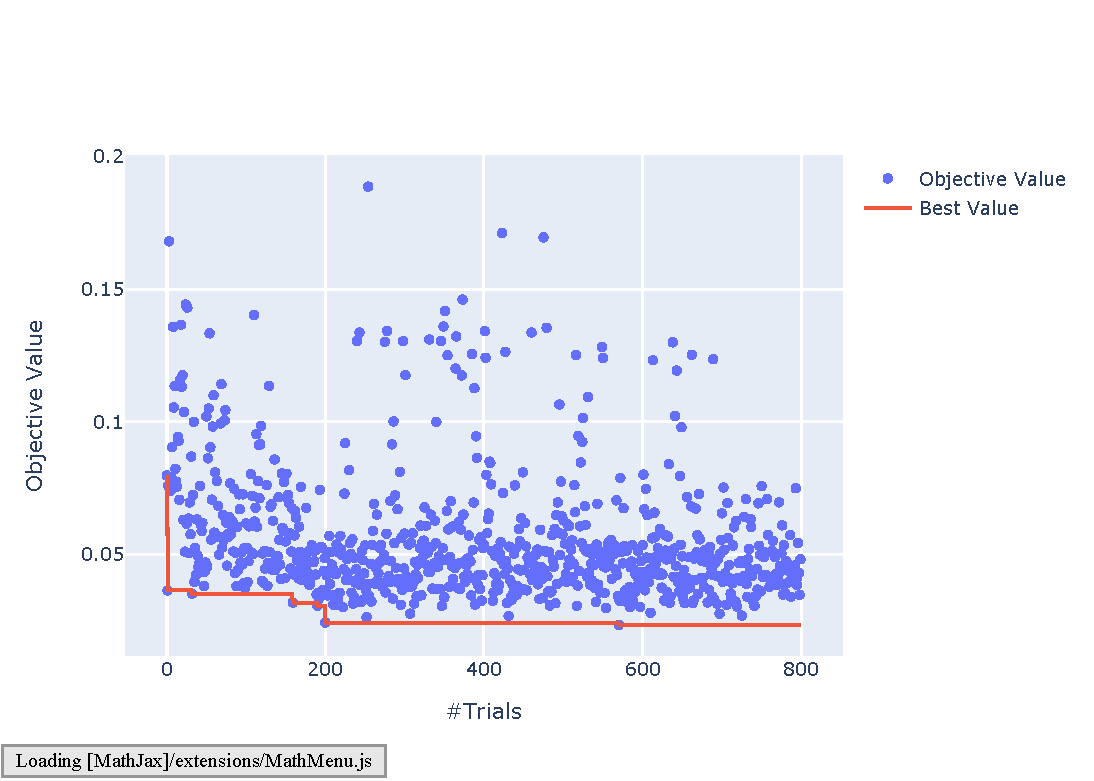
\includegraphics[width=.7\linewidth]{../plots/overall/Optimization_History_dolphin.pdf}
    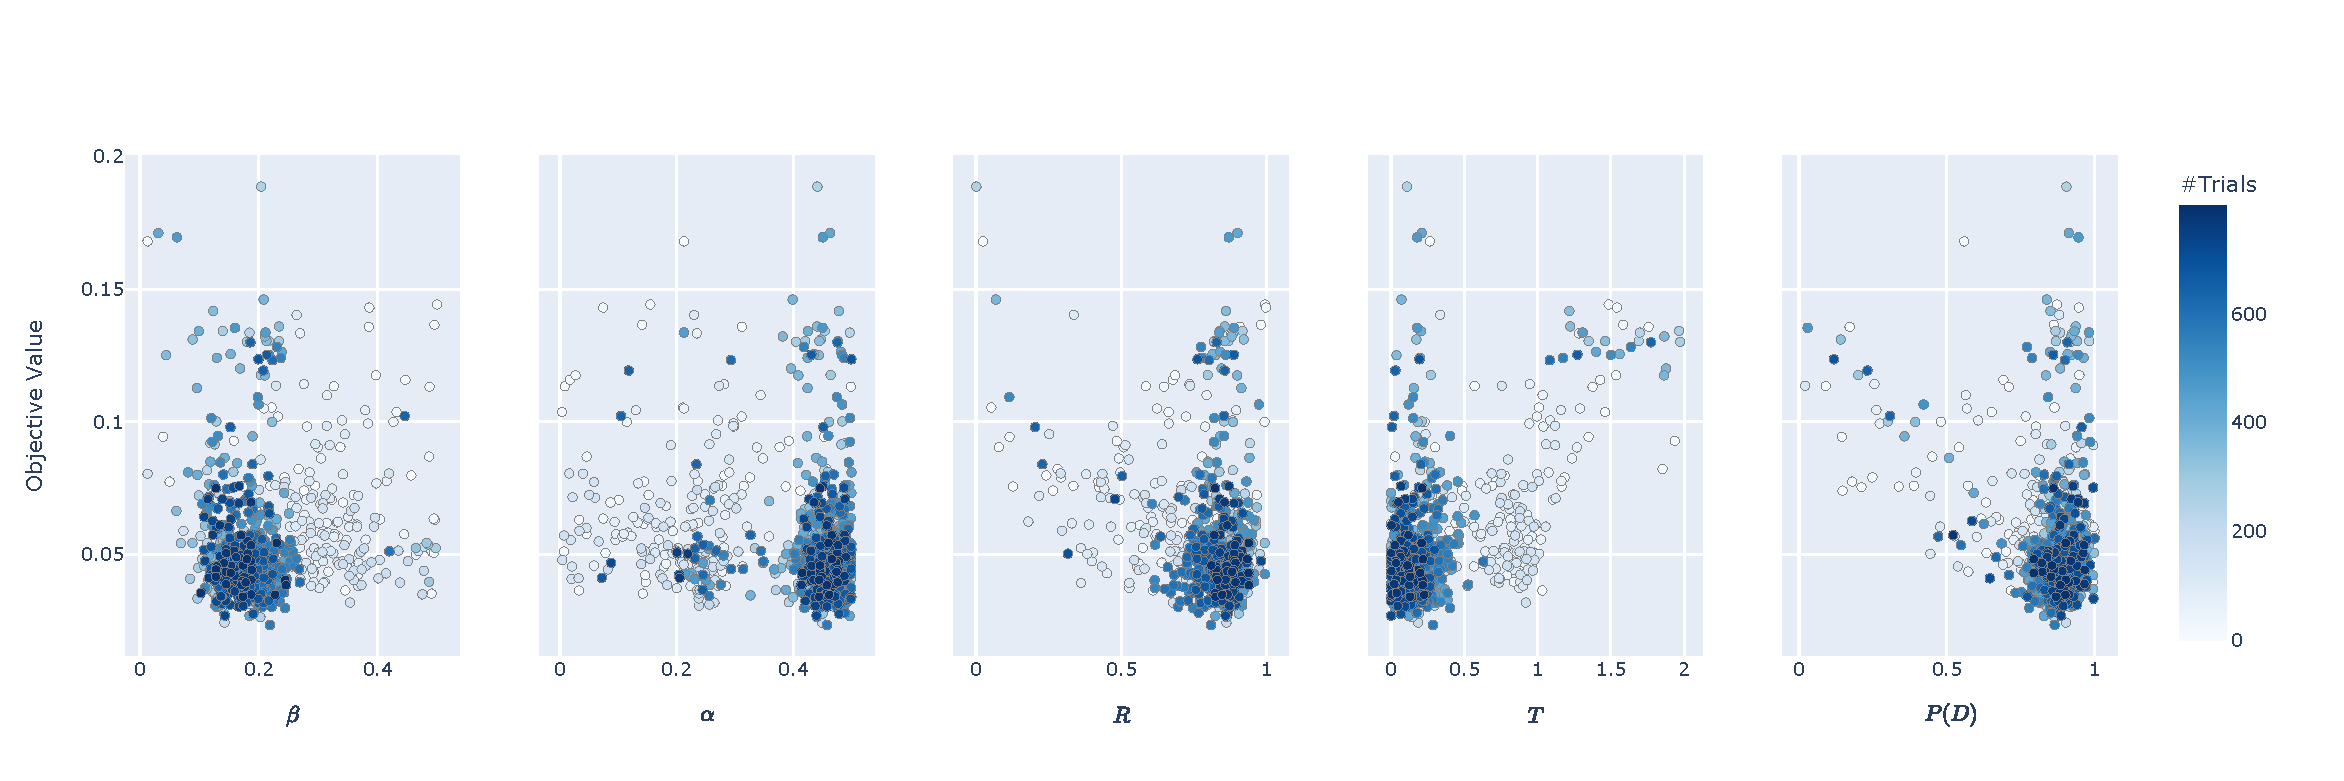
\includegraphics[width=.7\linewidth]{../plots/overall/Plot_Slice_dolphin.pdf}
  \caption{Diagnostic plots of optimization for the Dolphin Network. The plot on the first row shows the optimization history, with the x-axis showing the trial number and the y-axis showing the objective value of that trial. The red line shows the best value, blue dots show the objective value of each trial. The second row shows the search pattern for each parameter. The different columns show different model parameters. The x-axis for all columns shows the parameter's value. The y-axis shows the objective value. The dots are colored as a gradient by the trial number with darker colors indicating later trials.}
  \label{appendix:optimization_dolphin}
\end{figure}

\begin{figure}[H]
    \centering
    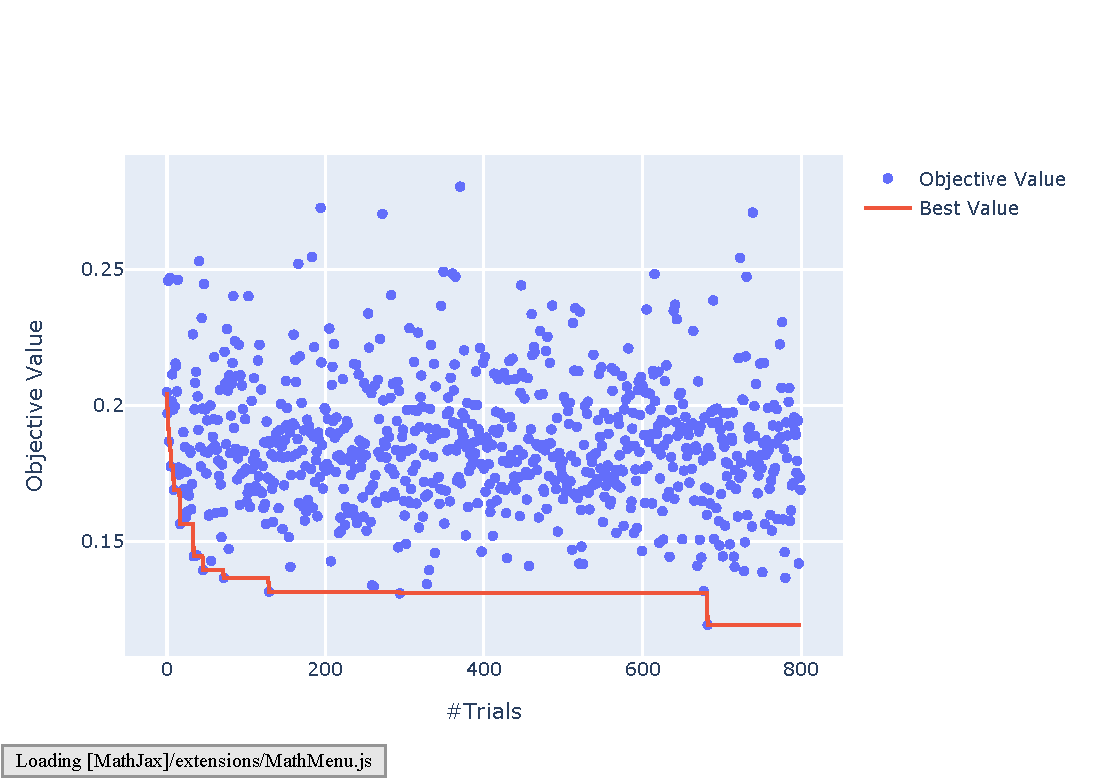
\includegraphics[width=.7\linewidth]{../plots/overall/Optimization_History_karate.pdf}
    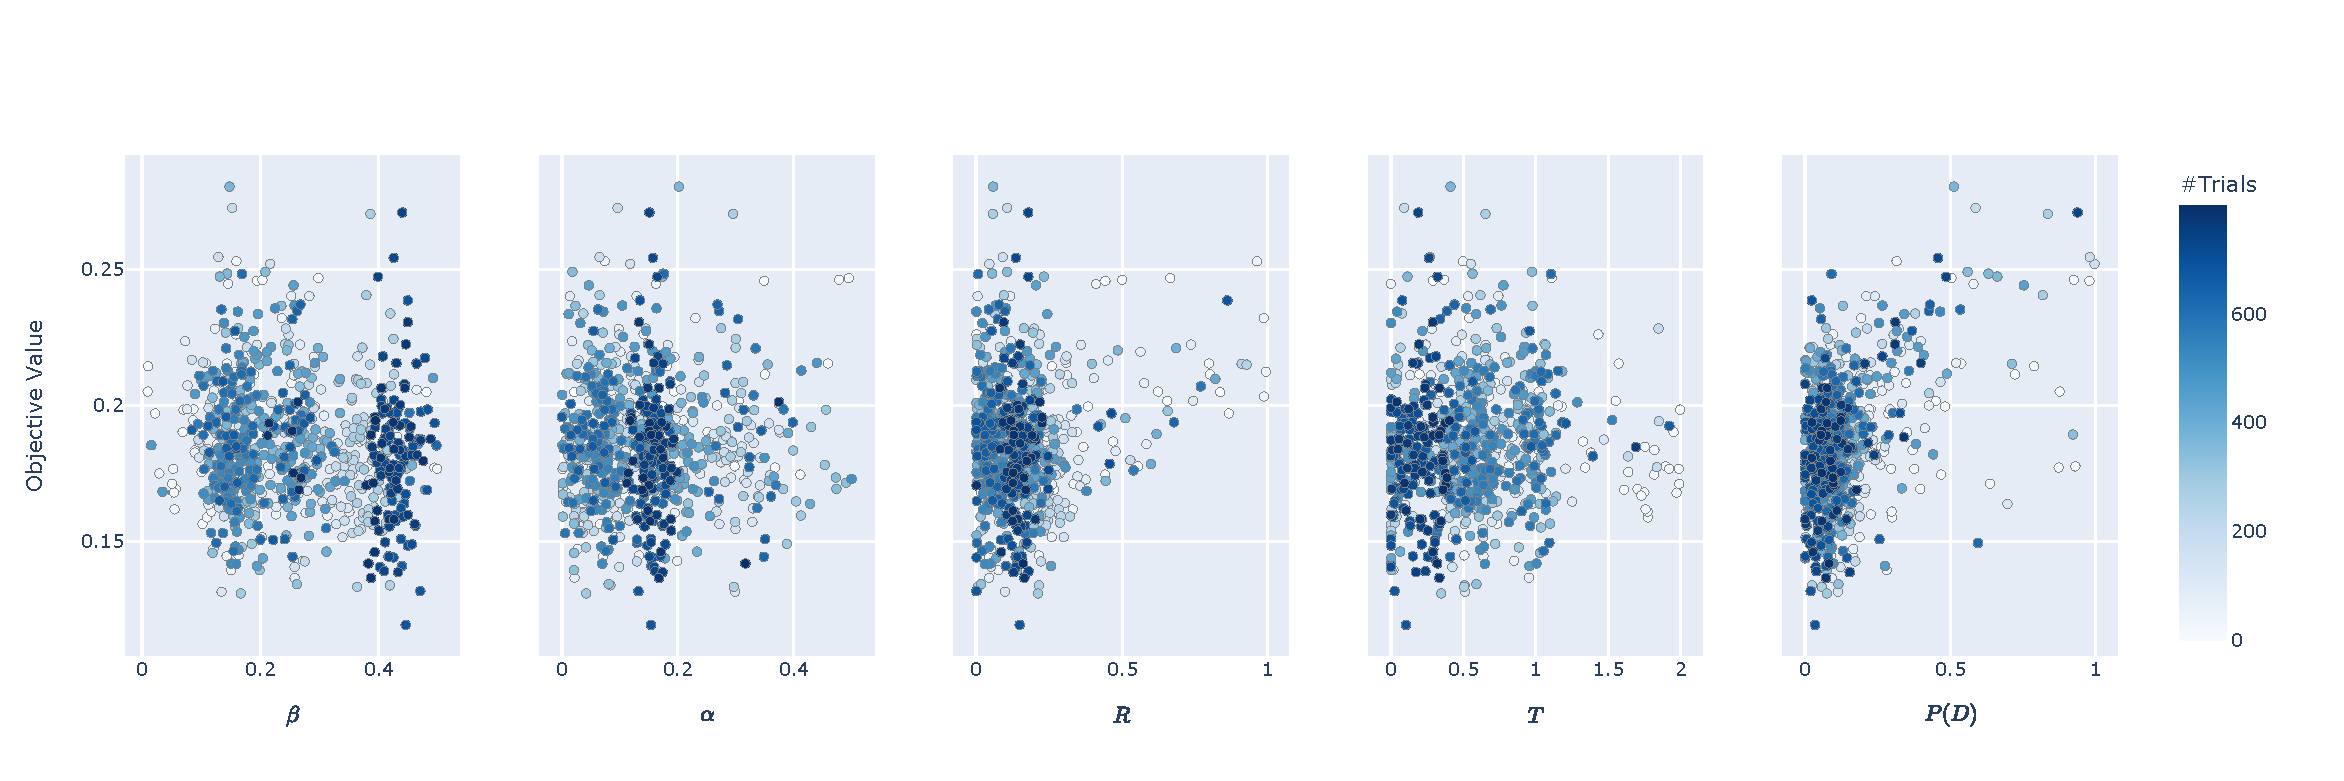
\includegraphics[width=.7\linewidth]{../plots/overall/Plot_Slice_karate.pdf}
  \caption{Diagnostic plots of optimization for the Karate Club Network. The plot on the first row shows the optimization history, with the x-axis showing the trial number and the y-axis showing the objective value of that trial. The red line shows the best value, blue dots show the objective value of each trial. The second row shows the search pattern for each parameter. The different columns show different model parameters. The x-axis for all columns shows the parameter's value. The y-axis shows the objective value. The dots are colored as a gradient by the trial number with darker colors indicating later trials.}
  \label{appendix:optimization_karate}
\end{figure}

\begin{figure}[H]
    \centering
    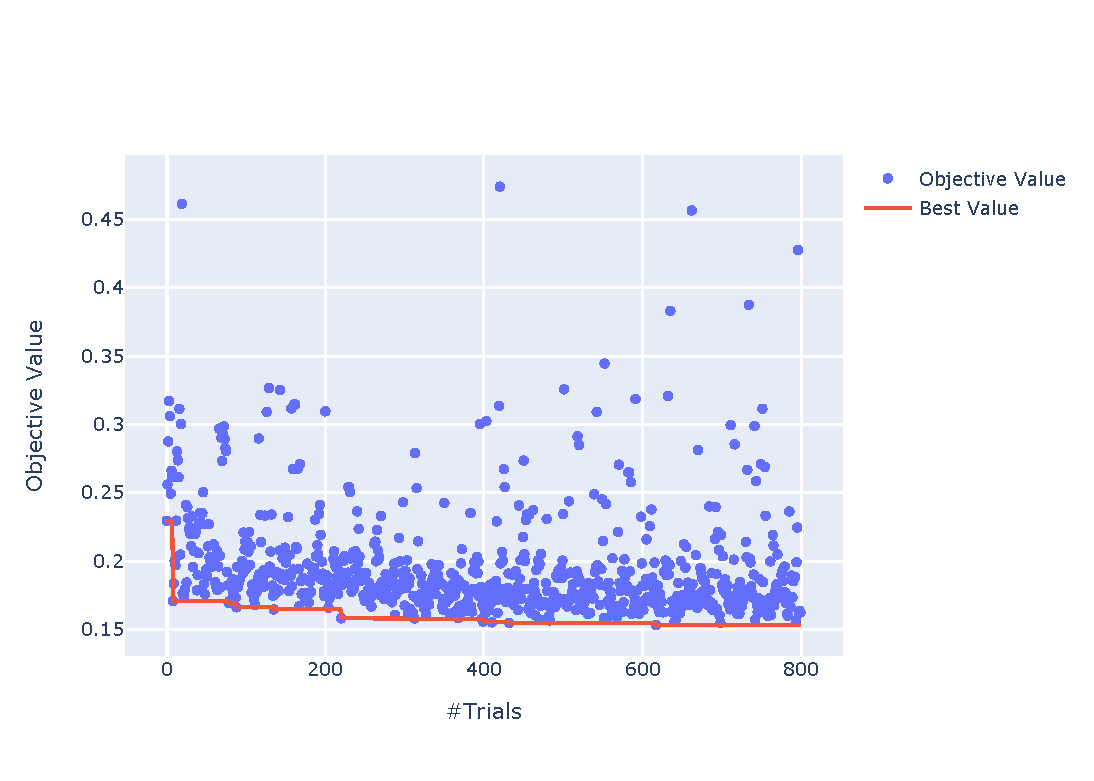
\includegraphics[width=.7\linewidth]{../plots/overall/Optimization_History_netscience.pdf}
    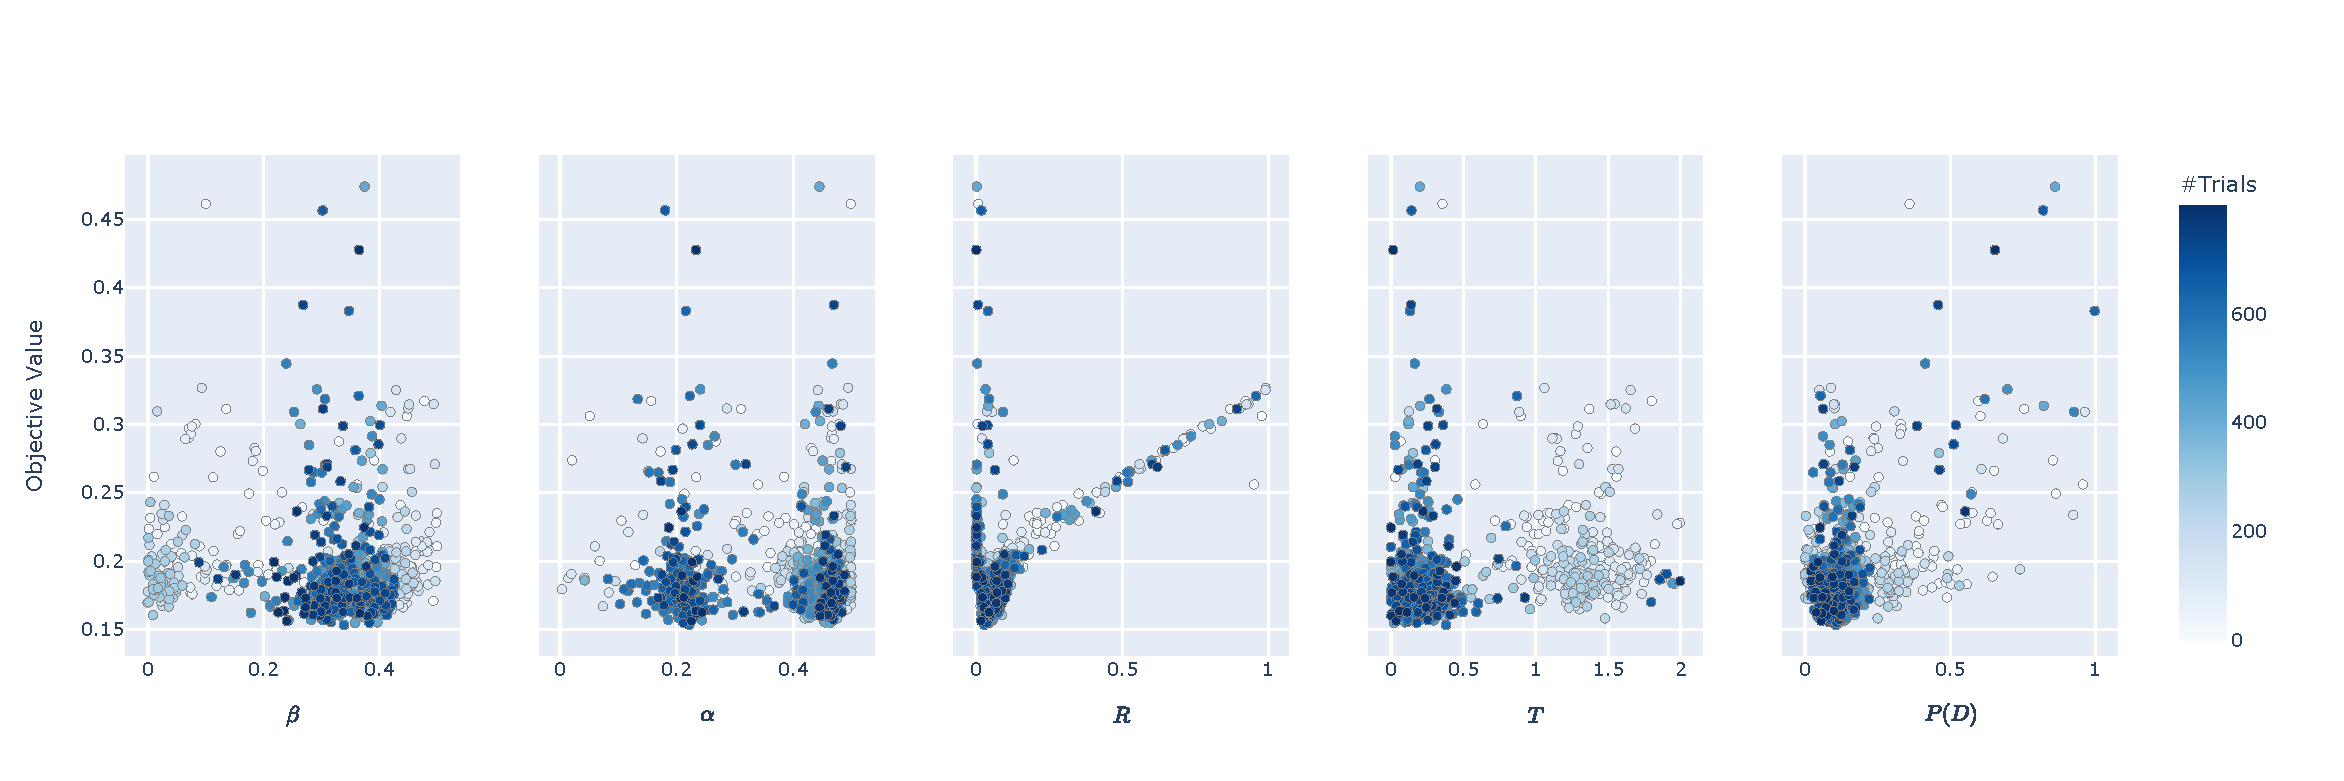
\includegraphics[width=.7\linewidth]{../plots/overall/Plot_Slice_netscience.pdf}
  \caption{Diagnostic plots of optimization for the Citation Network. The plot on the first row shows the optimization history, with the x-axis showing the trial number and the y-axis showing the objective value of that trial. The red line shows the best value, blue dots show the objective value of each trial. The second row shows the search pattern for each parameter. The different columns show different model parameters. The x-axis for all columns shows the parameter's value. The y-axis shows the objective value. The dots are colored as a gradient by the trial number with darker colors indicating later trials.}
  \label{appendix:optimization_netscience}
\end{figure}

\begin{figure}[H]
    \centering
    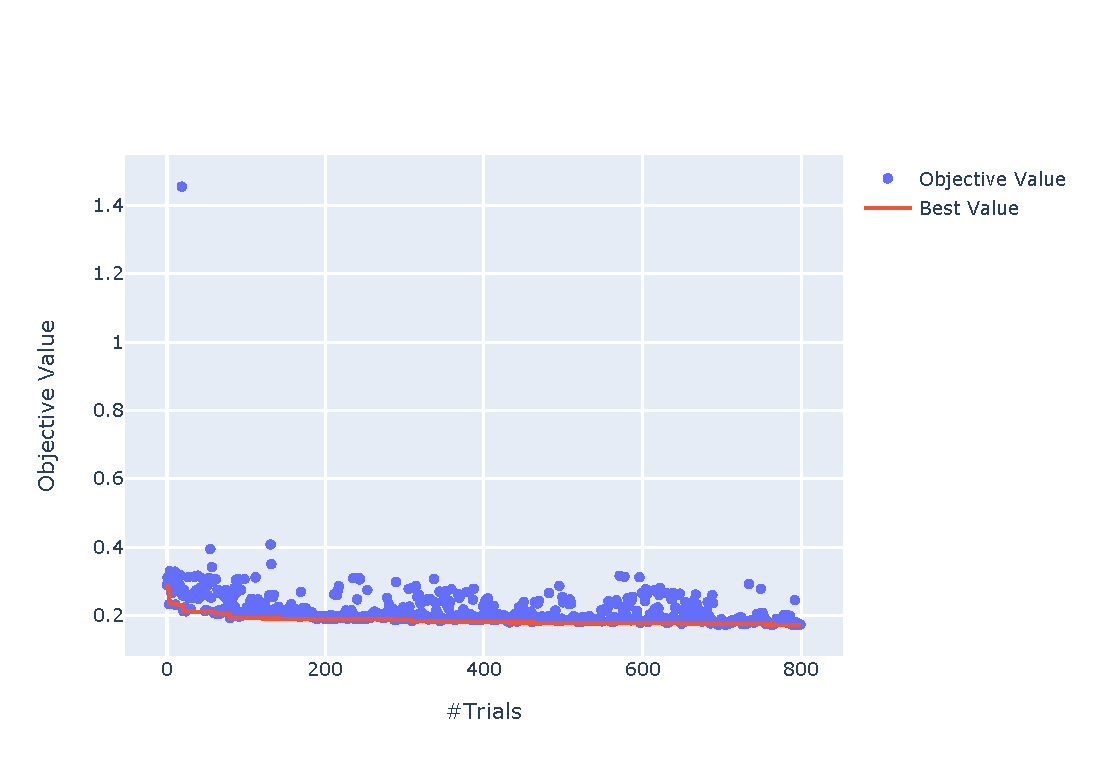
\includegraphics[width=.7\linewidth]{../plots/overall/Optimization_History_polblogs.pdf}
    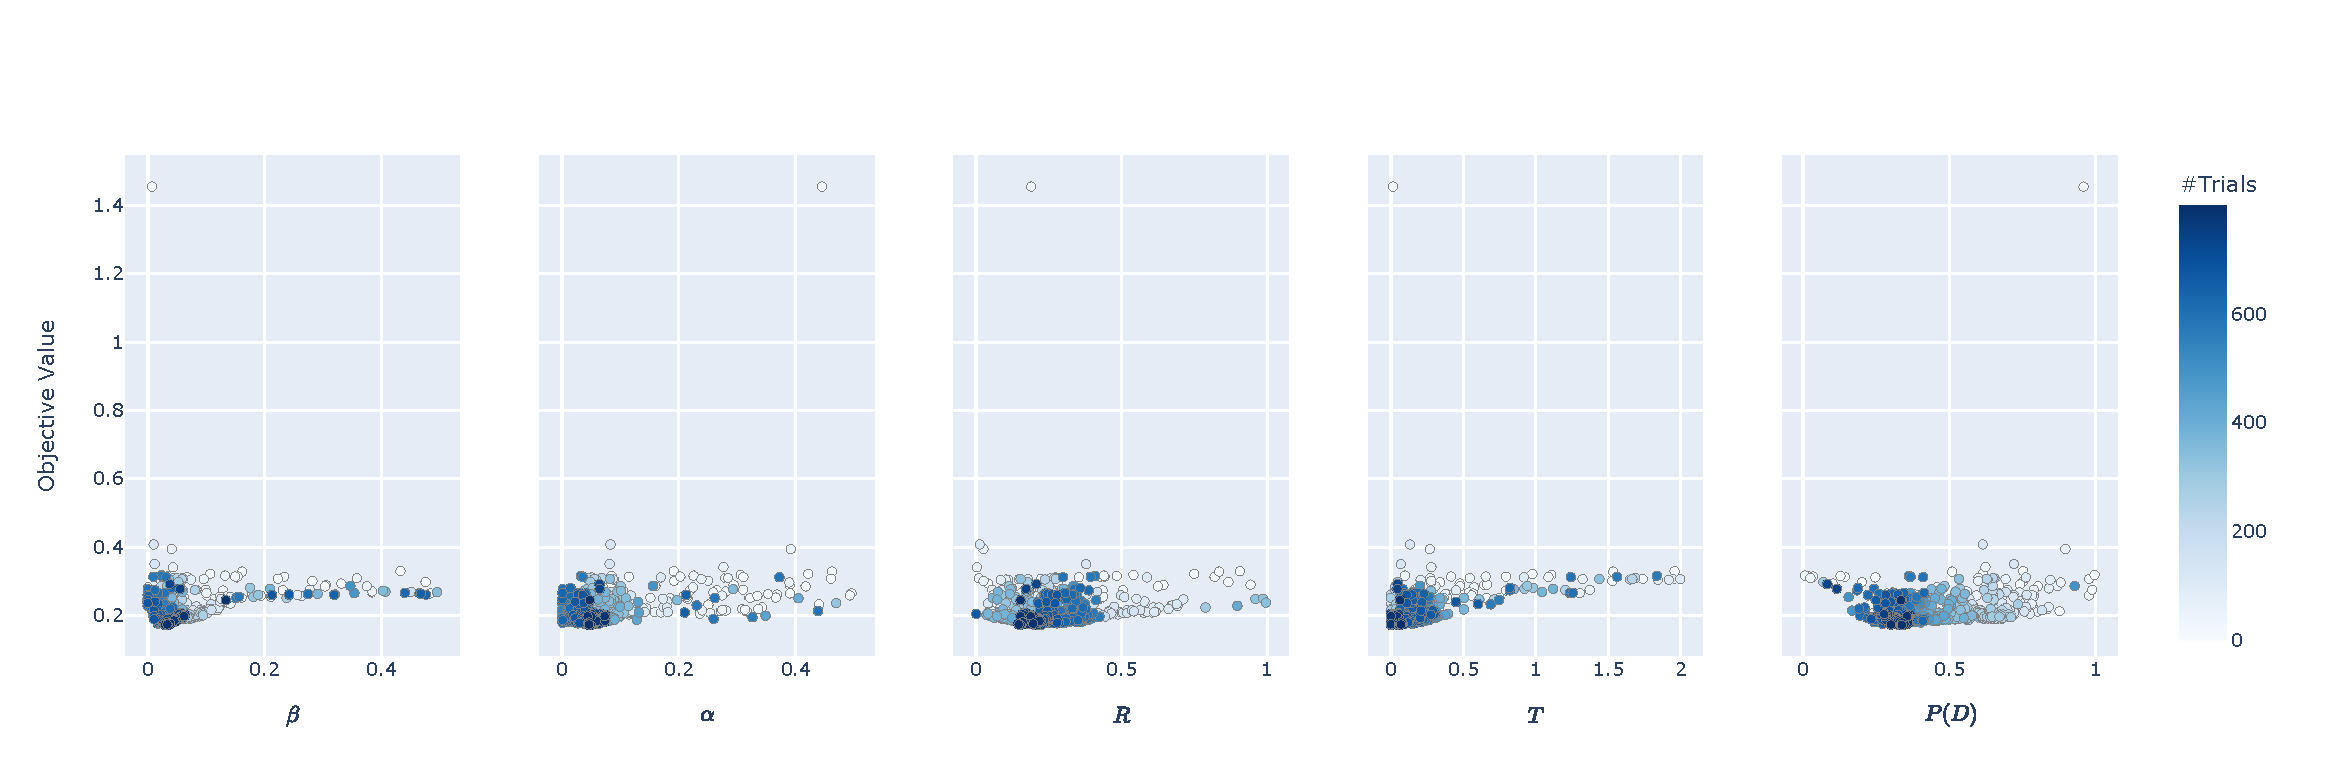
\includegraphics[width=.7\linewidth]{../plots/overall/Plot_Slice_polblogs.pdf}
  \caption{Diagnostic plots of optimization for the Political Blogs Network. The plot on the first row shows the optimization history, with the x-axis showing the trial number and the y-axis showing the objective value of that trial. The red line shows the best value, blue dots show the objective value of each trial. The second row shows the search pattern for each parameter. The different columns show different model parameters. The x-axis for all columns shows the parameter's value. The y-axis shows the objective value. The dots are colored as a gradient by the trial number with darker colors indicating later trials.}
  \label{appendix:optimization_polblogs}
\end{figure}

\begin{figure}[H]
    \centering
    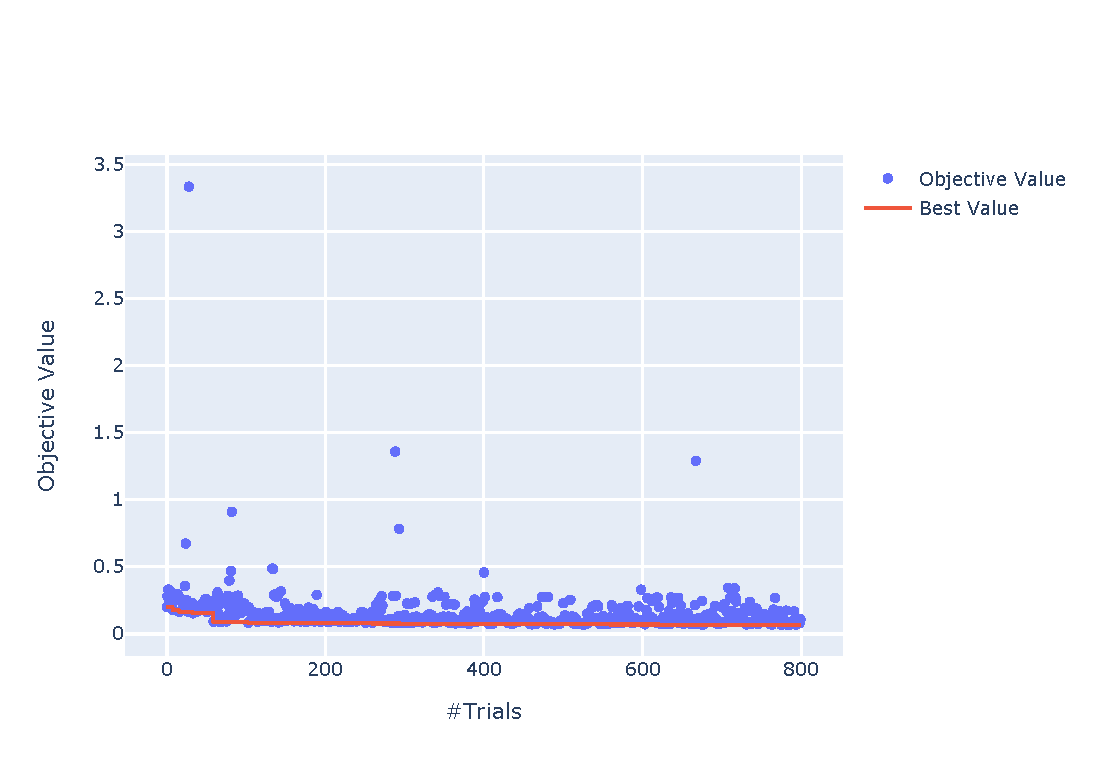
\includegraphics[width=.7\linewidth]{../plots/overall/Optimization_History_politicians.pdf}
    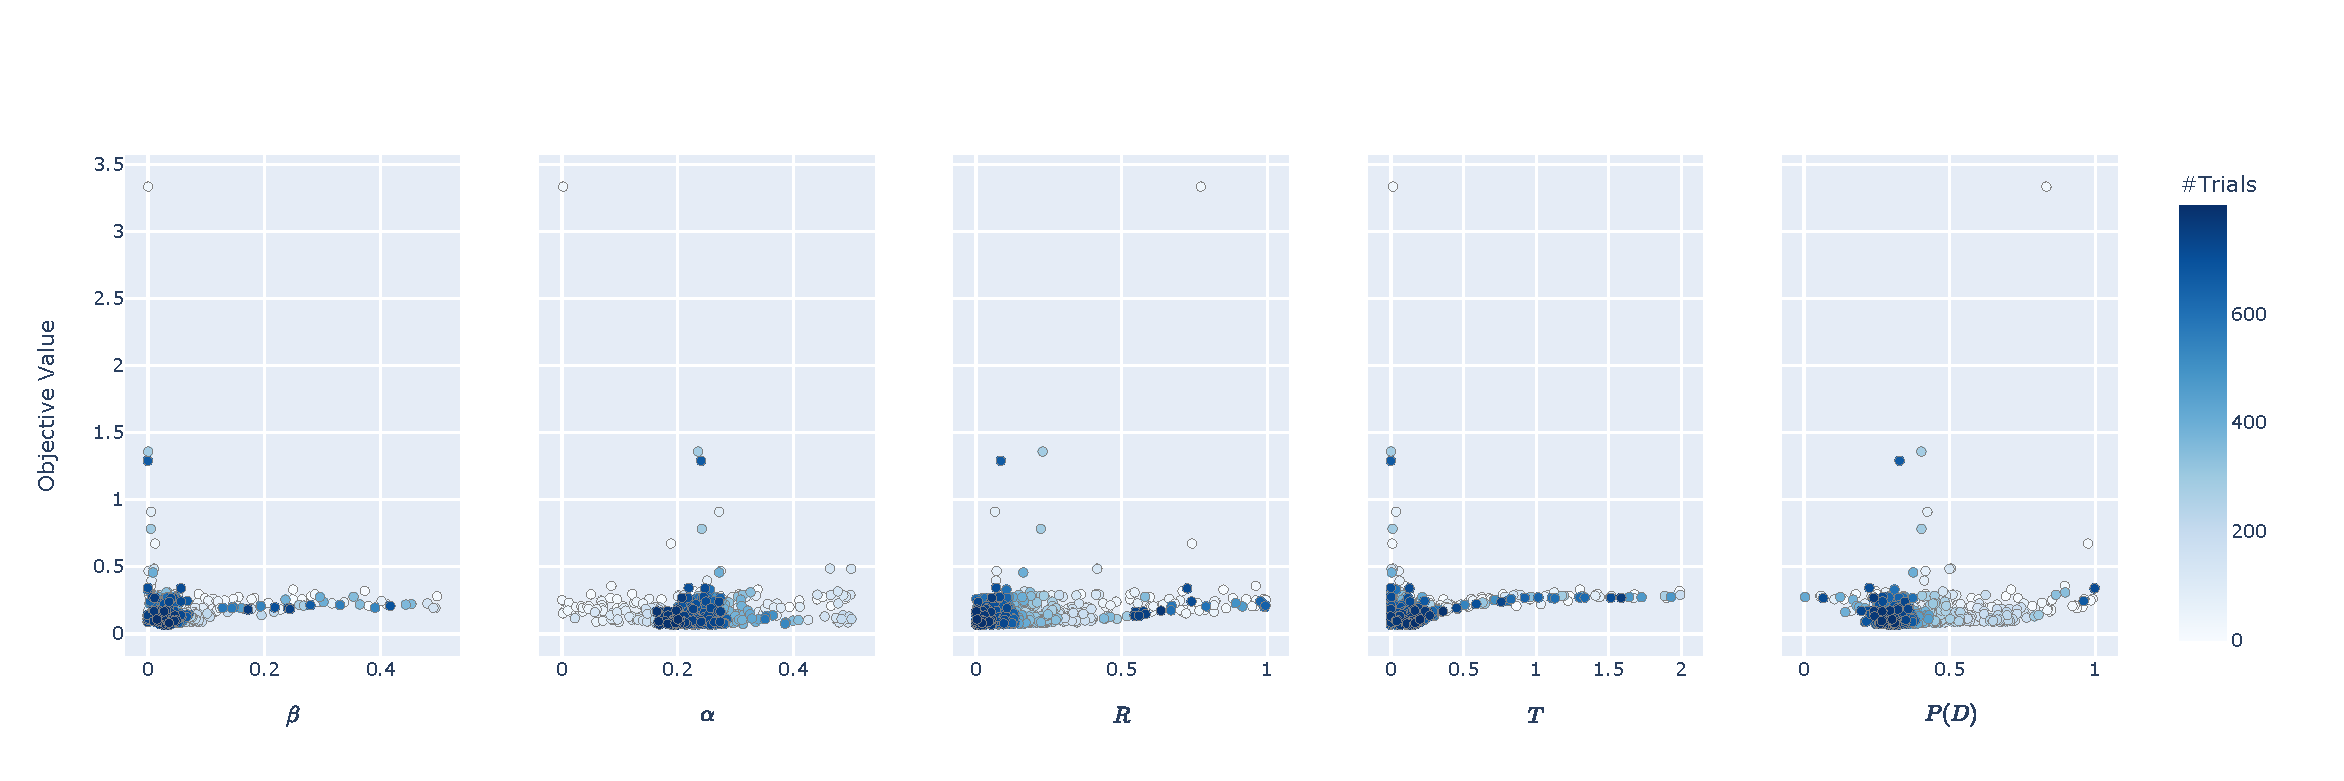
\includegraphics[width=.7\linewidth]{../plots/overall/Plot_Slice_politicians.pdf}
  \caption{Diagnostic plots of optimization for the Politicians Network. The plot on the first row shows the optimization history, with the x-axis showing the trial number and the y-axis showing the objective value of that trial. The red line shows the best value, blue dots show the objective value of each trial. The second row shows the search pattern for each parameter. The different columns show different model parameters. The x-axis for all columns shows the parameter's value. The y-axis shows the objective value. The dots are colored as a gradient by the trial number with darker colors indicating later trials.}
  \label{appendix:optimization_politicians}
\end{figure}

\begin{figure}[H]
    \centering
    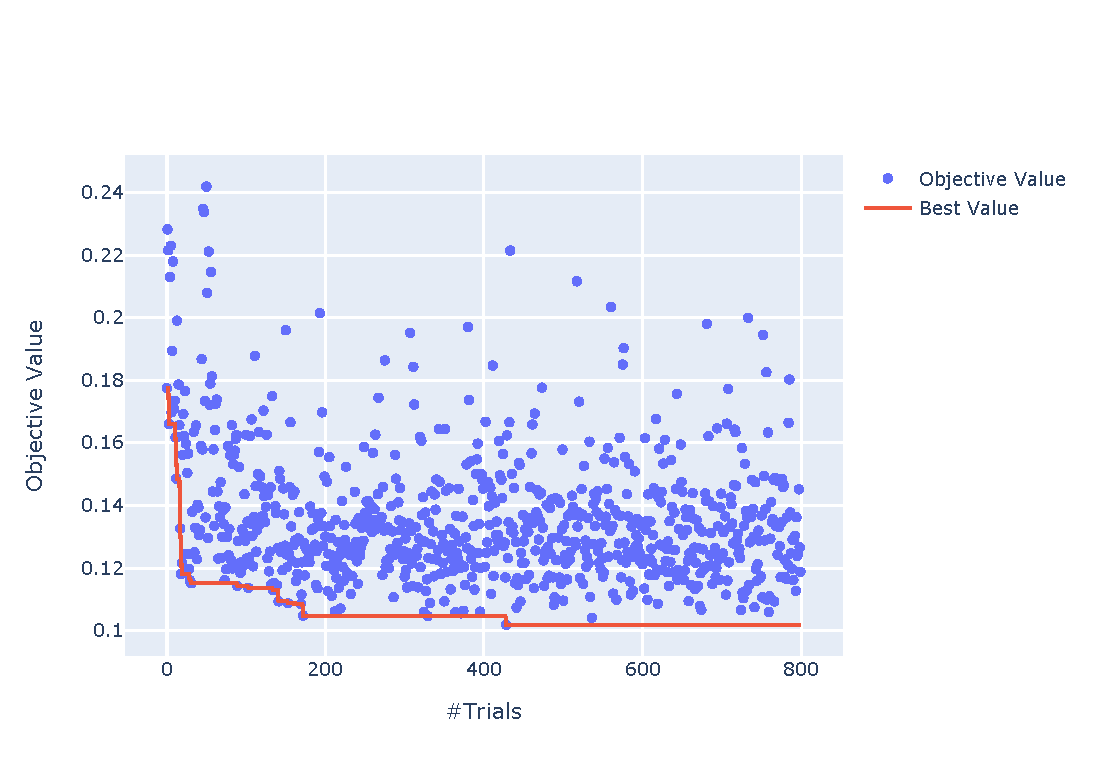
\includegraphics[width=.7\linewidth]{../plots/overall/Optimization_History_polbooks.pdf}
    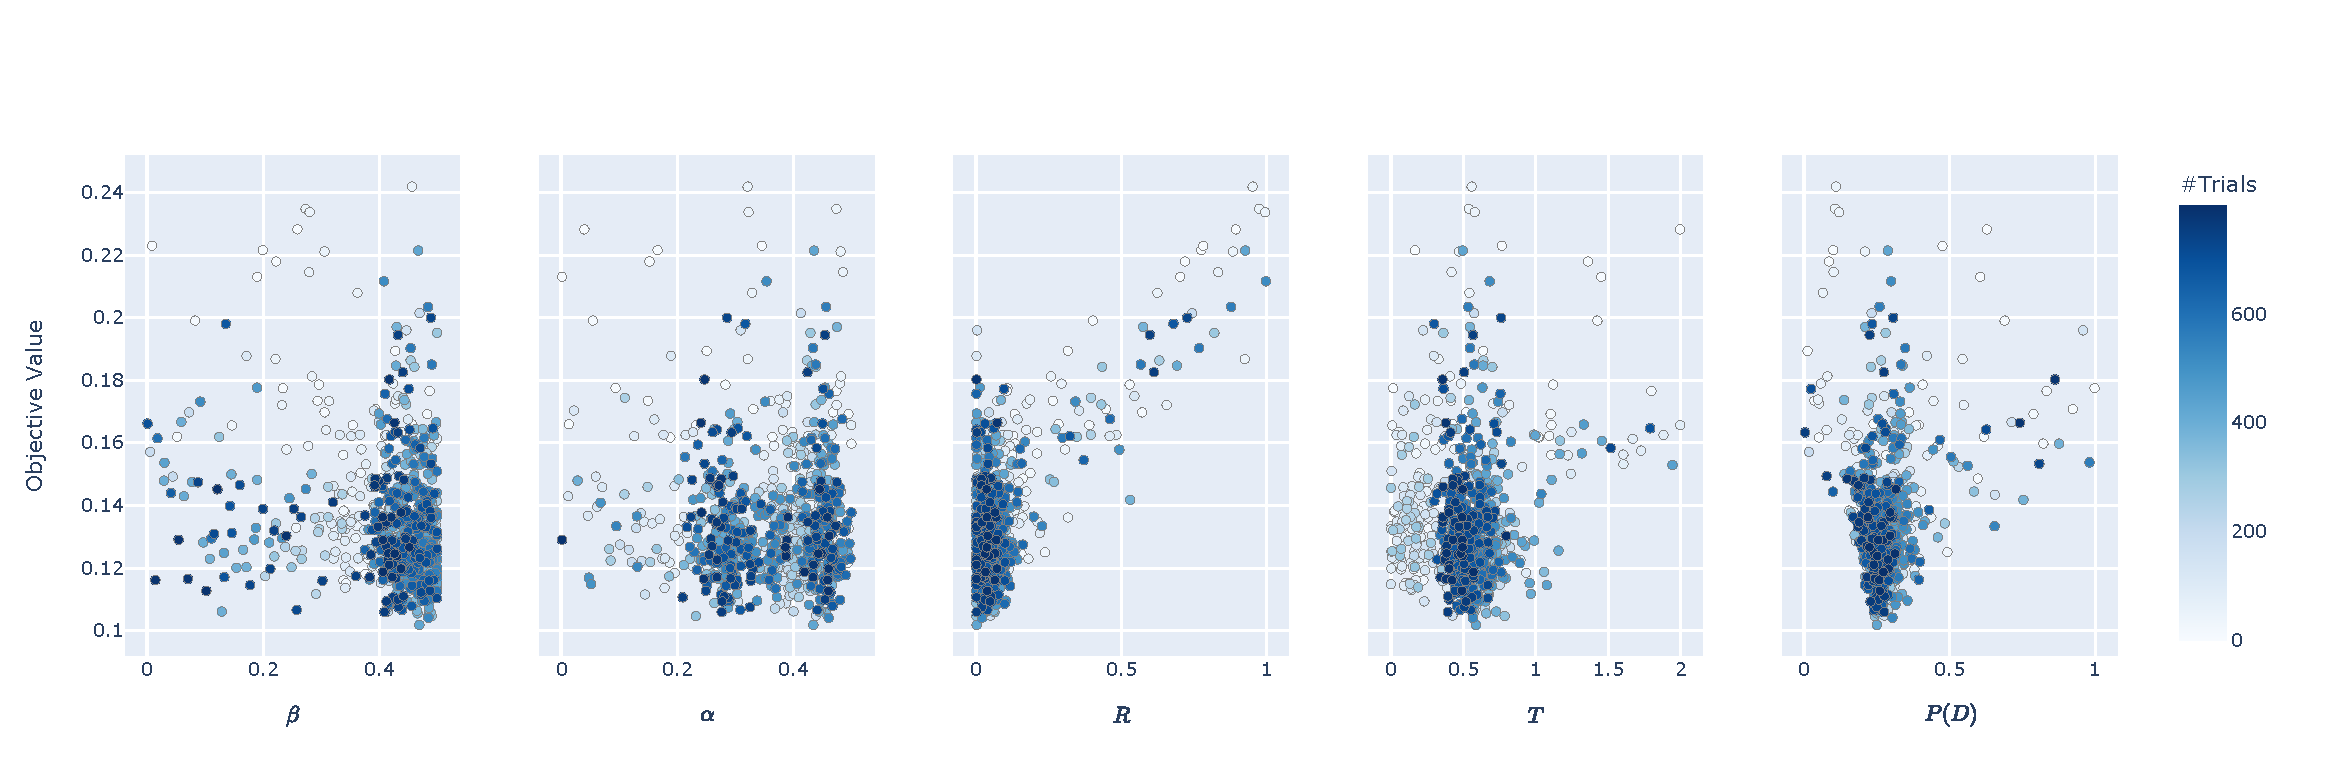
\includegraphics[width=.7\linewidth]{../plots/overall/Plot_Slice_polbooks.pdf}
  \caption{Political Books}
  \label{appendix:optimization_polbooks}
\end{figure}

\begin{figure}[H]
    \centering
    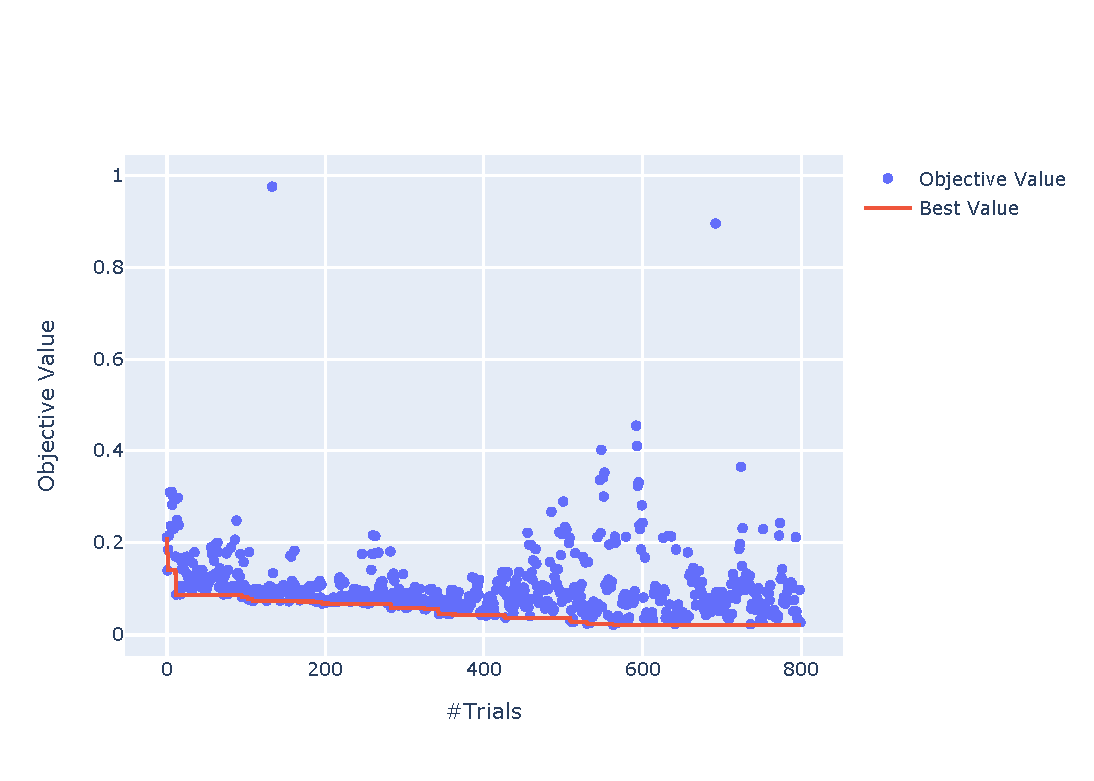
\includegraphics[width=.7\linewidth]{../plots/overall/Optimization_History_tvshows.pdf}
    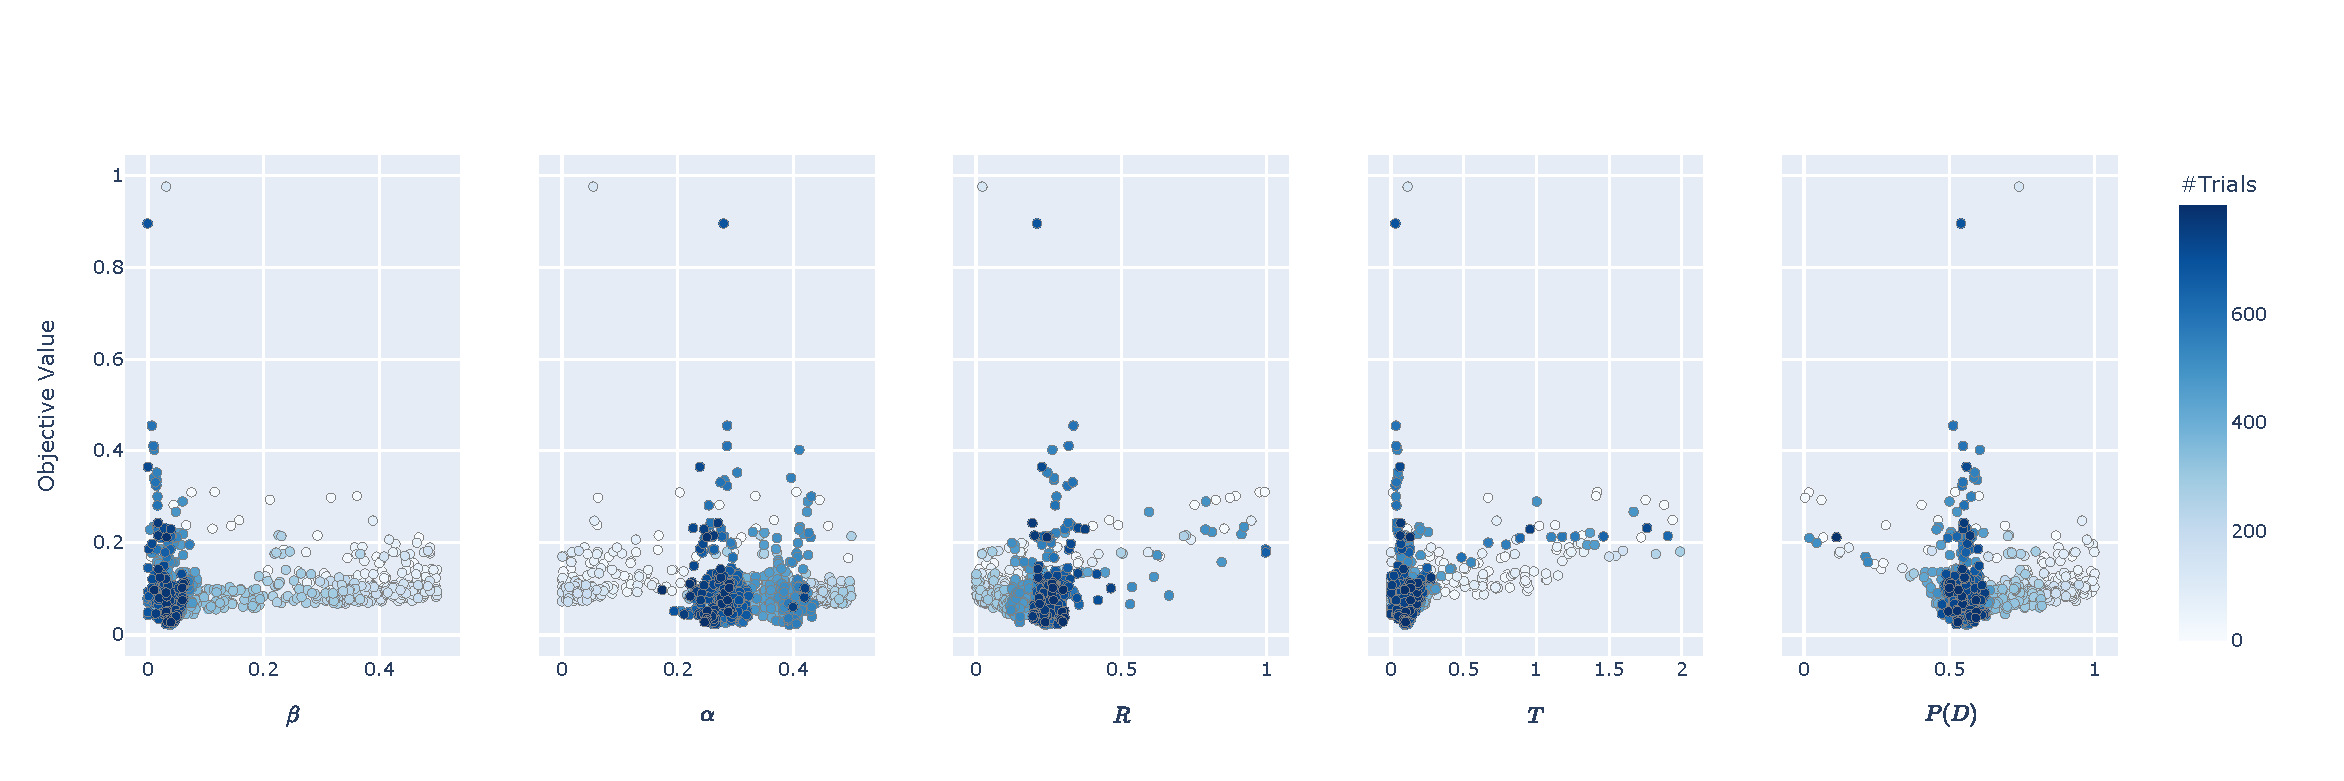
\includegraphics[width=.7\linewidth]{../plots/overall/Plot_Slice_tvshows.pdf}
  \caption{Diagnostic plots of optimization for the TV Shows Network. The plot on the first row shows the optimization history, with the x-axis showing the trial number and the y-axis showing the objective value of that trial. The red line shows the best value, blue dots show the objective value of each trial. The second row shows the search pattern for each parameter. The different columns show different model parameters. The x-axis for all columns shows the parameter's value. The y-axis shows the objective value. The dots are colored as a gradient by the trial number with darker colors indicating later trials.}
  \label{appendix:optimization_tvshows}
\end{figure}

\subsubsection{Metrics of model performance}
\begin{figure}[H]
    \centering
    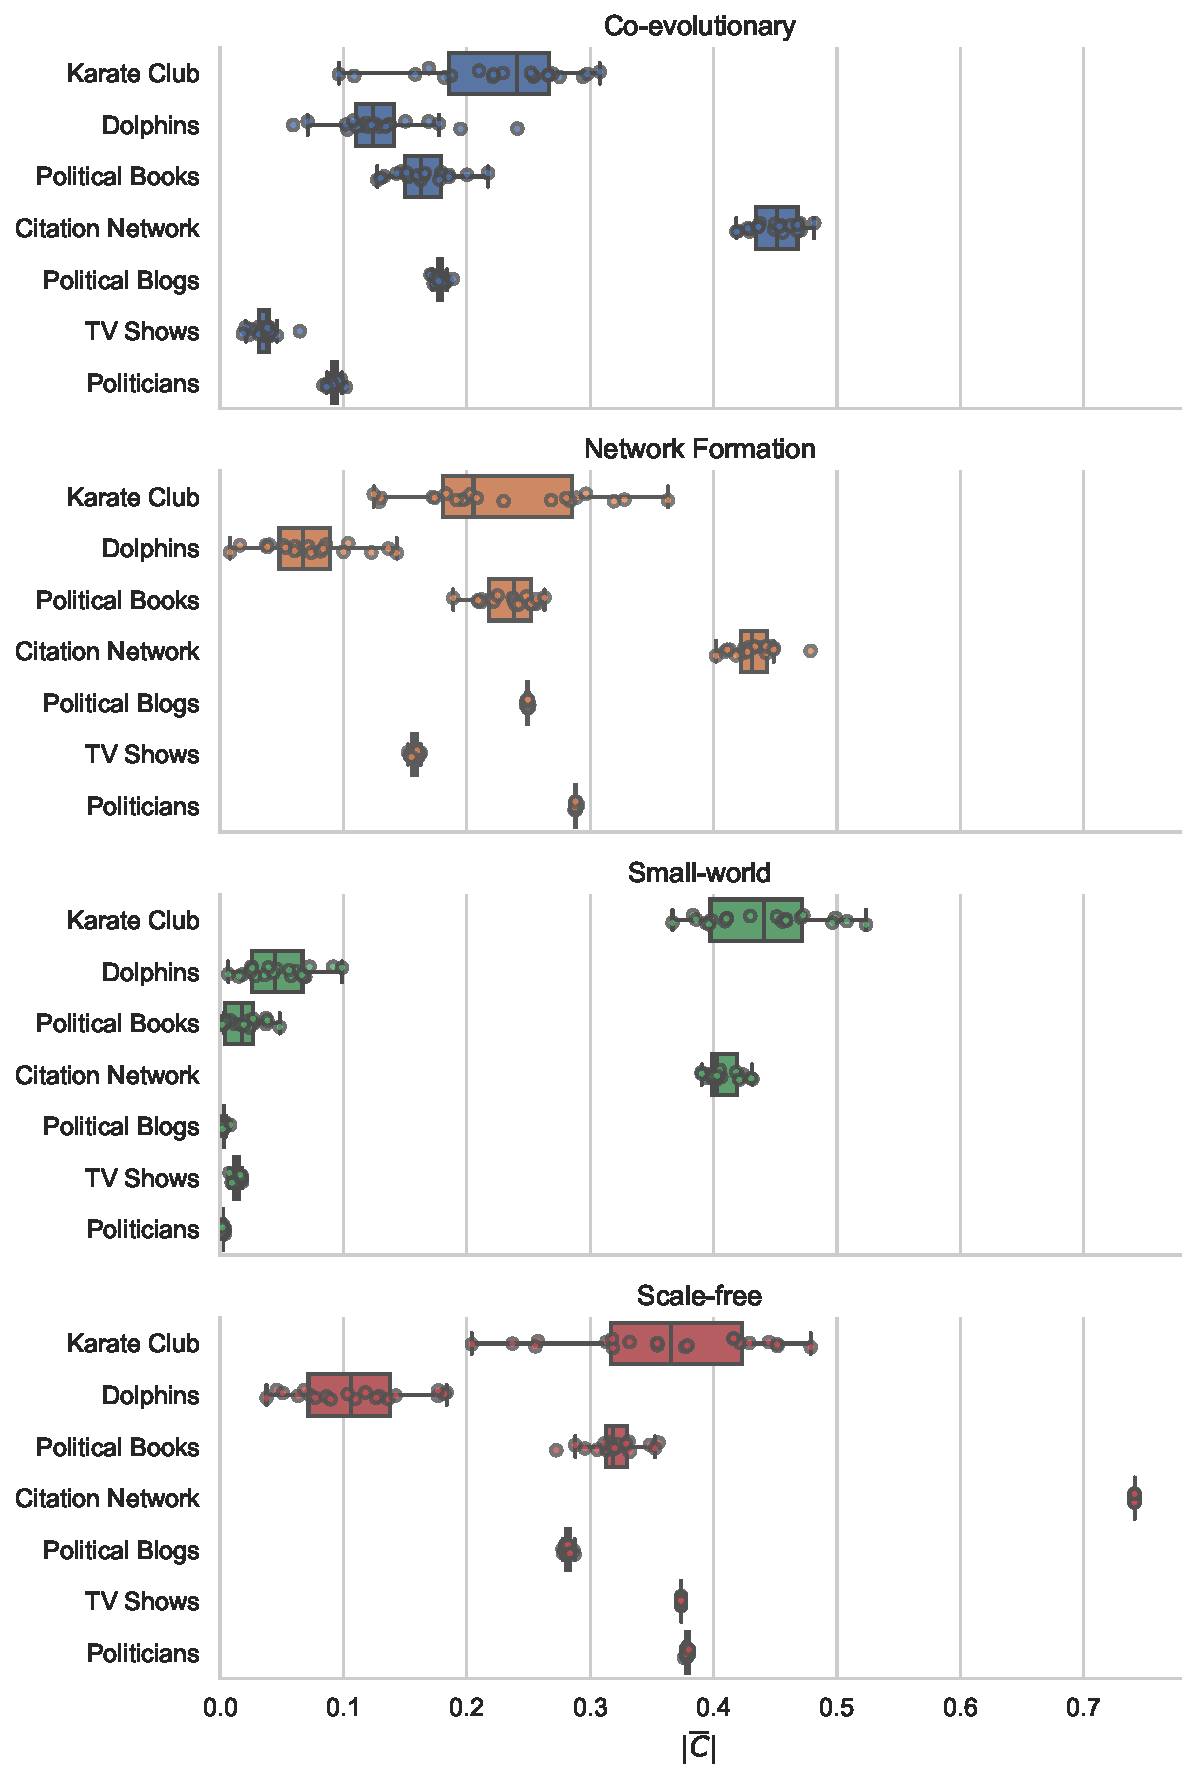
\includegraphics[width=.9\linewidth]{../plots/overall/Model_Evaluation_Average_Clustering.pdf}
  \caption{Difference between models and target regarding average clustering coefficient. The x-axis shows the difference between the average clustering coefficient of the generated and the empirical networks, $\overline{C}$. The y-axis shows the different empirical networks considered. Colors show different algorithms for generating networks. The vertical dashed line shows the value 0.0, the point of no difference between the generated and the empirical network. The dots show the result from individual simulations, while box plots show the median and quartiles of the distribution of values.}
  \label{appendix:eval_clustering}
\end{figure}

\begin{figure}[H]
    \centering
    \includegraphics[width=.9\linewidth]{../plots/overall/Model_Evaluation_APL.pdf}
  \caption{Difference between models and target regarding average path length. The x-axis shows the difference between the average path length of the generated and the empirical networks, $\overline{C}$. The y-axis shows the different empirical networks considered. Colors show different algorithms for generating networks. The vertical dashed line shows the value 0.0, the point of no difference between the generated and the empirical network. The dots show the result from individual simulations, while box plots show the median and quartiles of the distribution of values.}
  \label{appendix:eval_path}
\end{figure}

\begin{figure}[H]
    \centering
    \includegraphics[width=.9\linewidth]{../plots/overall/Model_Evaluation_JSD.pdf}
  \caption{Difference in degree distributions of generated and empirical networks. The x-axis shows the Jensen Shannon Divergence, $JSD$, of the degree distribution between the generated and the target network. The colors show different algorithms for generating networks. The y-axis shows the different empirical networks considered. The dots show the result from individual simulations, while box plots show the median and quartiles of the distribution of values.}
  \label{appendix:eval_divergence}
\end{figure}

\subsection{Supplementary information for co-evolution's effect on opinion dynamics}

\begin{figure}[H]
    \centering
    \includegraphics[width=.7\linewidth]{../plots/overall/Absolute_Opinion_Threshold.pdf}
  \caption{The effect of the threshold on polarization over time. The x-axis shows the time-steps and the y-axis shows the absolute value of the opinions of agents. Colors indicate different values of $T$. Lines indicate the mean value of each time-step, aggregated over all parameters excluding $T$. Shaded regions are the 95\% confidence intervals.}
  \label{appendix:threshold}
\end{figure}

\begin{figure}[H]
    \centering
    \includegraphics[width=.7\linewidth]{../plots/overall/Absolute_Opinion_Positive_Learning_Rate.pdf}
  \caption{The effect of positive social influence on polarization over time. The x-axis shows the time-steps and the y-axis shows the absolute value of the opinions of agents. Colors indicate different values of $\alpha$. Lines indicate the mean value of each time-step, aggregated over all parameters excluding $\alpha$. Shaded regions are the 95\% confidence intervals.}
  \label{appendix:alpha}
\end{figure}

\begin{figure}[H]
    \centering
    \includegraphics[width=.7\linewidth]{../plots/overall/Absolute_Opinion_Negative_Learning_Rate.pdf}
  \caption{The effect of negative social influence on polarization over time. The x-axis shows the time-step and the y-axis shows the absolute value of the opinions of agents. Colors indicate different values of $\beta$. Lines indicate the mean value of each time-step, aggregated over all parameters excluding $\beta$. Shaded regions are the 95\% confidence intervals.}
  \label{appendix:beta}
\end{figure}

\begin{figure}[H]
    \centering
    \includegraphics[width=.9\linewidth]{../plots/overall/Average_Clustering_Coefficient_Ties_Deleted.pdf}
  \caption{Average clustering coefficient over time. The x-axis shows time-steps, and the y-axis shows the average clustering coefficient of the network. The colors indicate different probabilities for negative tie deletion. The lines show the average value over all other parameters than $P(D)$ and $R$. The shaded areas indicate 95\% confidence intervals. Each panel shows different values of $R$.}
  \label{appendix:clustering}
\end{figure}

\begin{figure}[H]
    \centering
    \includegraphics[width=.9\linewidth]{../plots/overall/Standard_Deviation_Absolute_Opinion_Tie_Deletion.pdf}
  \caption{The effect of tie-deletion on the variance of opinions over time. The x-axis shows the time-steps and the y-axis shows the standard deviation of the absolute value of opinions. The colors indicate different probabilities of tie-deletion of dissimilar agents. The lines indicate the mean value of each time-step, aggregated over all parameters excluding the probability of tie-deletion. The shaded regions are the 95\% confidence intervals. }
  \label{appendix:pd_sd}
\end{figure}

\begin{figure}[H]
    \centering
    \includegraphics[width=.7\linewidth]{../plots/overall/Distance_Tie_Deletion.pdf}
  \caption{Average distance to neighbors' opinions. The different colors show different values of the probability of tie-deletion ($P(D)$). The x-axis shows the time-steps and the y-axis shows the mean distance to neighbors' opinions ($d_O$). }
  \label{appendix:distance}
\end{figure}

\begin{figure}[H]
    \centering
    \includegraphics[width=.98\linewidth]{../plots/overall/Point_Of_No_Return.pdf}
  \caption{Polarized, consensus, and in-between conditions. The x-axis shows time-steps, and the y-axis shows the average of the absolute value of opinions, $\abs{O}$. Colors indicate whether simulations ended in consensus, polarization, or something in-between. Different simulations were categorized into these different categories depending $\abs{O}$ at the 10.000th time-step. Conditions were labelled consensus if $\abs{O} \leq 0.2$, in-between if $0.2 < \abs{O} < 0.8$ and polarized if $0.8 \leq \abs{O}$. Areas on the plot were made by coloring the area between the minimum and the maximum value for every time-step.}
  \label{appendix:ponr}
\end{figure}

\begin{figure}[H]
    \centering
    \includegraphics[width=.7\linewidth]{../plots/example/Example_Negative_Ties_Deleted.pdf}
  \caption{Negative ties deleted in representative simulations over time. The x-axis shows time-steps, $t$, and the y-axis shows the cumulative frequency of negative ties deleted, $NTD$. Colors indicate different levels of randomness, $R$. Lines show single simulations using the same random seed over time. These simulations had parameter values of $T = 0.8$, $\alpha = 0.15$, $\beta = 0.1$ and $P(D)=1$.}
  \label{appendix:example_ntd}
\end{figure}

\begin{figure}[H]
    \centering
    \includegraphics[width=.98\linewidth]{../plots/overall/Average_Path_Length_Ties_Deleted.pdf}
  \caption{The effect of tie-deletion on the average path length over time. The x-axis shows the time-steps, $t$, and the y-axis shows the estimated average path length of the simulated network, $APL$. Colors indicate different probabilities of tie-deletion of dissimilar agents, $P(D)$. Lines indicate the mean value of each time-step, aggregated over all parameters excluding the probability of tie-deletion, $P(D)$ and randomness, $R$. Shaded regions are the 95\% confidence intervals. The three different plots show the different values of the probability of new connections being generated randomly, $R$. }
  \label{appendix:apl}
\end{figure}

\subsection{The effect of initial opinions}
The correlation between the initial opinion and the final opinion of agents, $\rho_{O_I, O_F}$, is dictated by the values of $\beta$ and $T$. When $\beta$ is low and $T$ is high, there is little correlation between initial and final opinions. When $\beta$ is high and $T$ is low, final and initial values are highly correlated (see Appendix~\ref{appendix:corr_initial_final}).

The conditions where there is a strong positive correlation between initial and final opinions are conditions with the combination of strong negative social influence,$\beta \geq 0.15$, and lower threshold values, $T \leq 1$ (see Appendix~\ref{appendix:corr_initial_final}). These conditions are likely to lead to high degrees of polarization. The results indicate that in polarized conditions, agents will tend to move less than in conditions where agents reach consensus. In conditions where agents do reach a consensus, your starting position does not matter much. The final opinion of agents will by definition be very similar to all other agents. However, in polarizing conditions, polarization is primarily caused by negative social influence. These simulations are simulations with parameter values of $\beta \gg 0$. Under such conditions, the initial opinion and the final opinion of agents correlate positively. This is mainly due to the fact that agents will tend to move across the aisle, but be pushed to the nearest extreme (see Figure~\ref{fig:lineplot}). Therefore, the initial opinion of agents becomes predictive of which extreme they will end up with. 

\begin{figure}[H]
    \centering
    \includegraphics[width=.8\linewidth]{../plots/overall/Correlation_Initial_Opinions.pdf}
  \caption{Correlations between initial opinions and final opinions. The x-axis shows different values of threshold, $T$, and the y-axis shows the Pearson Correlation Coefficient between the initial and final opinion of agents, $\rho_{O_I, O_F}$. Boxes indicate the quartiles and whiskers indicate the 1.5 of the inter-quartile range outside of the quartiles. Points outside this range are depicted as diamonds. Smaller dark dots show the correlation coefficient for individual simulations. Columns show low, medium, and high values of $\beta$. }
  \label{appendix:corr_initial_final}
\end{figure}

\end{document}